\PassOptionsToPackage{hyphens}{url}
\documentclass[11pt,a4paper]{article}

%\usepackage[provide=*,spanish]{babel}
\usepackage[utf8]{inputenc}
\usepackage[spanish,es-nodecimaldot,es-tabla]{babel}
\usepackage[T1]{fontenc}
\usepackage{lmodern}
\usepackage[margin=2.35cm]{geometry}
\usepackage{amsmath}
\usepackage{amssymb}
\usepackage{booktabs}
\usepackage{longtable}
\usepackage{tabularx}
\usepackage{array}
\usepackage{enumitem}
\usepackage{listings}
\usepackage{xcolor}
\usepackage{microtype}
\usepackage{parskip}
\usepackage{titlesec}
\usepackage{hyperref}
\usepackage{graphicx}
\usepackage{caption}
\usepackage{float}
\usepackage{tocloft}
\setlength{\cftsecnumwidth}{2.2em}
\setlength{\cftsubsecnumwidth}{2.8em}
\setlength{\cftsubsubsecnumwidth}{3.6em}
\renewcommand{\cftsecfont}{\bfseries\color{azulWCD}}
\renewcommand{\cftsecpagefont}{\bfseries}

\definecolor{azulWCD}{RGB}{17,67,112}
\definecolor{grisCodigo}{RGB}{247,247,247}
\definecolor{verdeCodigo}{RGB}{25,110,55}
\definecolor{rojoCodigo}{RGB}{145,35,35}
\definecolor{tituloColor}{RGB}{0,55,110}
\definecolor{reglaColor}{RGB}{0,90,160}

\hypersetup{
  colorlinks=true,
  linkcolor=azulWCD,
  urlcolor=azulWCD,
  citecolor=azulWCD,
  pdftitle={Respuesta del WCD a flujos monocromáticos de neutrones},
  pdfauthor={Jaime A. Betancourt}
}

\lstdefinestyle{shstyle}{
  backgroundcolor=\color{grisCodigo},
  basicstyle=\ttfamily\footnotesize,
  breaklines=true,
  frame=single,
  rulecolor=\color{gray!40},
  columns=fullflexible,
  keepspaces=true
}
\lstset{style=shstyle}

\titleformat{\section}{\normalfont\Large\bfseries\color{azulWCD}}
  {\thesection.}{0.6em}{}
\titleformat{\subsection}{\normalfont\large\bfseries}
  {\thesubsection.}{0.5em}{}
\titleformat{\subsubsection}{\normalfont\normalsize\bfseries}
  {\thesubsubsection.}{0.5em}{}
\setlist{itemsep=0.25em,topsep=0.4em}
\renewcommand{\arraystretch}{1.18}
\setlength{\emergencystretch}{2em}
\captionsetup{font=small,labelfont=bf}

% Figuras del informe (procesamiento) y figuras de la Sección 4.2 regeneradas por el notebook
\graphicspath{{figuras-procesamiento-64-corridas/}{../../../analysis/campana-1_neutrones-monoenergeticos_seccion-4.2/figuras-seccion-4.2/}}
\newcommand{\tablaanalisis}{../../../analysis/campana-1_neutrones-monoenergeticos_seccion-4.2/figuras-seccion-4.2}

\newcommand{\codigo}[1]{\nolinkurl{#1}}
\newcommand{\archivo}[1]{\path{#1}}
\newcommand{\var}[1]{\texttt{#1}}
\newcommand{\ap}{\textcolor{red}{agua pura}}

\begin{document}
\pagestyle{empty}

\begin{titlepage}
\begin{center}

\vspace*{0.5cm}
\textcolor{reglaColor}{\rule{\linewidth}{1.2pt}}

\vspace{1.3cm}
{\Large\scshape Universidad Industrial de Santander}\\[0.2cm]
{\large Escuela de Física --- Facultad de Ciencias}\\[0.2cm]
{\large Doctorado en Física}

\vspace{2.2cm}
{\Huge\bfseries\color{tituloColor} Respuesta del WCD \\[0.2cm]
 a flujos\\[0.4cm] monocromáticos de neutrones}

\vspace{1.8cm}
{\large\textbf{Informe técnico}}

\vspace{0.6cm}
\begin{minipage}{0.82\linewidth}
\centering
\textit{``Transporte, moderación y captura de neutrones entre 1~meV y 1~keV en agua pura y en agua con NaCl: de los archivos crudos del simulador a los resultados de la Sección~4.2 de la tesis''}
\end{minipage}

\vfill

{\large\textbf{Autor}}\\[0.15cm]
Jaime A. Betancourt\\[0.1cm]
Doctorado en Física, Universidad Industrial de Santander

\vspace{1.2cm}
\textcolor{reglaColor}{\rule{0.5\linewidth}{0.6pt}}

\vspace{1cm}
6 de octubre de 2026

\vspace{1cm}
\textcolor{reglaColor}{\rule{\linewidth}{1.2pt}}

\end{center}
\end{titlepage}

\pagestyle{plain}

\begin{abstract}
Este informe reúne los resultados de la Sección~4.2 de la tesis sobre la respuesta del detector Cherenkov de agua (WCD) a flujos monocromáticos de neutrones, en lo que concierne al propio neutrón: su transporte, su moderación y su captura en el volumen detector. La base son las 64 corridas de la Campaña~1: dieciséis energías de inyección entre 1~meV y 1~keV, cuatro medios (agua pura y soluciones con 2.5, 5 y 10~\% de NaCl en masa), $10^5$ neutrones por corrida y física \texttt{QGSP\_BERT\_HP} sin $S(\alpha,\beta)$. Dos scripts del repositorio procesan los archivos crudos en alrededor de un minuto y reproducen exactamente las cifras de la tesis; un notebook regenera todas sus figuras. El informe presenta el número medio de pasos de transporte y de dispersiones elásticas, la distribución del número de dispersiones antes de la captura ($\langle N\rangle$ pasa de 44.8 a 76.8 entre 1~meV y 1~keV en agua pura), la letargía por colisión $\xi$ en los regímenes frío, térmico, epitérmico e intermedio, el balance de captura, reflexión, transmisión y otros destinos con su tratamiento estadístico multinomial (la captura en agua pura va de 17.4 a 35.9~\%, y el NaCl la eleva hasta 51.4~\%), la ganancia relativa de captura y la longitud de captura. La respuesta electromagnética posterior a la captura, la carga registrada por el fotomultiplicador y la eficiencia de detección se tratan en un informe técnico aparte; aquí se deja establecido el enlace entre ambos.
\end{abstract}

\tableofcontents

% =====================================================================
\section{Objeto y alcance}
\label{sec:objeto}

La Sección~4.2 de la tesis caracteriza la respuesta del WCD a neutrones monoenergéticos en dos etapas: lo que le ocurre al neutrón en el detector (transporte, moderación, captura y escape) y la cadena electromagnética y óptica que convierte cada captura en una señal (radiación gamma, partículas cargadas secundarias, luz Cherenkov y fotoelectrones). Este informe cubre la primera etapa:

\begin{enumerate}
  \item el transporte y la dispersión elástica de los neutrones (Figuras~4.17 y 4.18 de la tesis);
  \item la moderación: número de dispersiones elásticas antes de la captura (Figura~4.19 y Figuras~D.1--D.3) y letargía $\xi$ por régimen de energía (Figuras~4.20--4.23, Tabla~4.6 y Figuras~D.4--D.6);
  \item el balance de captura, reflexión, transmisión y otros destinos, con sus incertidumbres (Tablas~4.7 y 4.8, Figuras~4.24--4.26 y Apéndice~C);
  \item la ganancia relativa de captura con NaCl (Figura~4.27);
  \item la distribución espacial y la longitud de captura (Tabla~4.9 y Figuras~4.28 y 4.29).
\end{enumerate}

La respuesta electromagnética inducida por la captura, la carga por evento (Figuras~4.48 y 4.50) y la eficiencia de detección (Figura~4.51) se documentan en un informe técnico propio de esta misma carpeta; la Sección~\ref{sec:enlace} resume el enlace entre los dos informes.

Además de los resultados físicos, el informe documenta el procesamiento automatizado y verificable con que se obtuvieron: reconstruye todas las magnitudes por neutrón y por corrida desde los archivos crudos, sin archivos intermedios, verifica que las cifras de la tesis se reproducen y deja el método en el repositorio. Reemplaza al informe anterior de esta carpeta, \textit{Informe-tecnico-Analisis-Moderacion-Captura-Neutrones}, retirado del repositorio el 6 de octubre de 2026 (se conserva en el historial de git): analizaba un subconjunto anterior de cinco energías (1, 10, 25 y 100~meV y 10~keV), con otra copia de los datos, y clasificaba los destinos por las caras de la caja del mundo de Geant4 en lugar de las del volumen activo.

La Tabla~\ref{tab:correspondencia} relaciona las figuras y tablas de la tesis con las de este informe.

\begin{table}[H]
\centering
\small
\caption{Correspondencia entre la Sección~4.2 de la tesis y este informe. Las figuras de la tesis se regeneran con el notebook \texttt{figuras\_seccion\_4.2.ipynb} (Sección~\ref{sec:reproducibilidad}).}
\label{tab:correspondencia}
\begin{tabularx}{\linewidth}{@{}>{\raggedright\arraybackslash}p{3.3cm}>{\raggedright\arraybackslash}X>{\raggedright\arraybackslash}p{5.0cm}@{}}
\toprule
\textbf{Tesis} & \textbf{Contenido} & \textbf{Este informe} \\
\midrule
Fig.~4.17, 4.18 & Pasos \var{Transportation} y \var{hadElastic} por neutrón & Figs.~\ref{fig:transporte}, \ref{fig:hadelastic}; Tabla~\ref{tab:pasos} \\
Fig.~4.19, D.1--D.3 & $P(N\mid\text{captura})$ por medio & Figs.~\ref{fig:N-AP}--\ref{fig:N-NaCl}, \ref{fig:N-medio} \\
Fig.~4.20--4.23, D.4--D.6; Tabla~4.6 & Distribuciones de $\xi$ por régimen & Figs.~\ref{fig:xi-fria}--\ref{fig:xi-medio}; Tablas~\ref{tab:xi-fria}--\ref{tab:xi-intermedia}; Apéndice~\ref{ap:xi} \\
Tabla~4.7 & Propiedades de los medios & Tabla~\ref{tab:medios} \\
Fig.~4.24--4.26; Tabla~4.8; Apéndice~C & Coeficientes de captura, reflexión, transmisión y otros & Figs.~\ref{fig:captura}--\ref{fig:trans-otros}; Tabla~\ref{tab:coef-AP}; Apéndice~\ref{ap:tablas} \\
Fig.~4.27 & Ganancia relativa de captura & Fig.~\ref{fig:cap-rel} \\
Fig.~4.28, 4.29; Tabla~4.9 & Longitud de captura & Figs.~\ref{fig:lambda-1keV}, \ref{fig:lambda-E}; Tabla~\ref{tab:lambda} \\
Fig.~4.48--4.51 & Carga y eficiencia de detección & Informe de la respuesta electromagnética (Sección~\ref{sec:enlace}) \\
\bottomrule
\end{tabularx}
\end{table}

% =====================================================================
\section{Simulación y datos de entrada}
\label{sec:datos}

\subsection{Configuración de la simulación}

Cada corrida inyecta $N_\mathrm{inc}=10^5$ neutrones monoenergéticos en dirección vertical descendente desde $z_0=1.5$~m, dentro de un disco de 25~cm de radio centrado en el eje del tanque, unos 17~cm por encima de la cara interior de la tapa ($z=1330$~mm). El volumen activo es un cilindro de agua de 480~mm de radio y 1330~mm de altura ($V_\mathrm{det}=0.962694$~m$^3$). La física hadrónica es \texttt{QGSP\_BERT\_HP} sin el tratamiento $S(\alpha,\beta)$ de dispersión térmica, y el medio está a 20~$^\circ$C (293.15~K), de modo que $k_BT\simeq25.3$~meV. Las simulaciones son de febrero de 2025 y su código corresponde a la etiqueta \codigo{campana-1-QGSP_BERT_HP} del repositorio.

Las dieciséis energías cubren los cuatro regímenes de la clasificación de la tesis (Tabla~2.2):

\begin{center}
\small
\begin{tabular}{@{}lll@{}}
\toprule
\textbf{Régimen} & \textbf{Intervalo} & \textbf{Energías simuladas} \\
\midrule
Frío & 1--10~meV & 1, 2.5, 5, 7 y 10~meV \\
Térmico & 10--100~meV & 10, 25, 50, 80 y 100~meV \\
Epitérmico & 100~meV--1~eV & 100, 300, 500 y 700~meV y 1~eV \\
Intermedio & 1~eV--1~keV & 1, 10 y 100~eV y 1~keV \\
\bottomrule
\end{tabular}
\end{center}

El extremo superior coincide con el límite de $10^3$~eV de la ventana que Köhli et al.\ identifican como sensible al contenido de agua del suelo en aplicaciones CRNS~\cite{Kohli2015}.

\subsection{Medios detectores}

La Tabla~\ref{tab:medios} reproduce las propiedades de los cuatro medios usadas en la tesis. Las densidades provienen de los volúmenes específicos de soluciones acuosas de NaCl a 20~$^\circ$C y 1~bar de Rogers y Pitzer~\cite{Rogers1982}; la densidad numérica de hidrógeno $n_\mathrm{H}$ se obtiene de la densidad de la solución, su fracción másica de agua y la constante de Avogadro~\cite{Tiesinga2021}.

\begin{table}[H]
\centering
\small
\caption{Propiedades de los medios detectores agua--NaCl a 20~$^\circ$C (Tabla~4.7 de la tesis). Concentraciones en porcentaje másico; $M$ es la masa del volumen activo; $\Delta n_\mathrm{H}$ y $\Delta\mathrm{H}$ se calculan respecto al agua pura.}
\label{tab:medios}
\begin{tabular}{@{}lrrrrr@{}}
\toprule
\textbf{Medio} & $\rho$ [kg\,m$^{-3}$] & $M$ [kg] & $n_\mathrm{H}$ [$10^{22}$\,cm$^{-3}$] & $\Delta n_\mathrm{H}$ [$10^{20}$\,cm$^{-3}$] & $\Delta\mathrm{H}$ [\%] \\
\midrule
Agua pura & 998.20 & 960.96 & 6.67356 & 0 & 0 \\
Agua + 2.5~\% NaCl & 1016.04 & 978.14 & 6.62301 & 5.055 & 0.757 \\
Agua + 5~\% NaCl & 1034.01 & 995.44 & 6.56732 & 10.624 & 1.592 \\
Agua + 10~\% NaCl & 1070.51 & 1030.57 & 6.44129 & 23.226 & 3.480 \\
\bottomrule
\end{tabular}
\end{table}

El NaCl aumenta la densidad y reduce el hidrógeno como máximo en un 3.5~\%. Esa reducción no le quita al medio su carácter moderador: por su masa cercana a la del neutrón, el hidrógeno sigue dominando la pérdida de energía por dispersión elástica. Lo que cambia de forma apreciable es la absorción, por la gran sección eficaz del $^{35}$Cl.

\subsection{Archivos crudos}

Las corridas están en la carpeta \archivo{Neutrones-termicos/energia/medio/} del equipo del autor. Las carpetas \codigo{1000meV}, \codigo{10000meV}, \codigo{100000meV} y \codigo{1000000meV} se rotulan en la tesis como 1~eV, 10~eV, 100~eV y 1~keV, y los medios son \codigo{Agua-pura}, \codigo{Agua+2.5NaCl}, \codigo{Agua+5NaCl} y \codigo{Agua+10NaCl}. Las 64 carpetas contienen los mismos archivos:

\begin{center}
\begin{tabularx}{\linewidth}{@{}lX@{}}
\toprule
\textbf{Archivo} & \textbf{Contenido} \\
\midrule
\archivo{interaccion-completa-neutrones.txt} & Un paso del neutrón primario por línea: número de paso, partícula, \textit{track}, padre, $E_\mathrm{pre}$ [MeV], posición previa $(x_0,y_0,z_0)$ y posterior $(x_1,y_1,z_1)$ [mm], $E_\mathrm{post}$ [MeV] y proceso. Una historia empieza cuando el número de paso vuelve a 1. \\
\archivo{neutrones-capturados.txt} & Posición y energía de cada captura. Se usa solo para verificar. \\
\archivo{Carga_Total_*.txt} & Número de fotoelectrones de cada evento con señal en el PMT (usado en el informe de la respuesta electromagnética). \\
\bottomrule
\end{tabularx}
\end{center}

El archivo de partículas secundarias de la captura (\archivo{secondary-particles-neutron-capturado.txt}) solo existe en la carpeta de 1~meV en agua pura; los espectros gamma de la tesis provienen de otro conjunto de datos.

\textbf{Verificación de la inyección.} En las 64 corridas, la primera línea registra $z_0=1500$~mm y una energía $E_0$ igual al valor nominal de la carpeta.

% =====================================================================
\section{Método}
\label{sec:metodo}

\subsection{Procesamiento en una sola pasada}

El script \archivo{procesar_corrida.py} recorre \archivo{interaccion-completa-neutrones.txt} una sola vez. Para cada historia acumula sus pasos y, al cerrarla, calcula todas las magnitudes; en paralelo alimenta la máquina de estados que reproduce la definición de $N$ de la tesis (Sección~\ref{sec:N}). El script \archivo{procesar_campana.py} lo ejecuta sobre las 64 corridas en paralelo y reúne los resúmenes.

\subsection{Destino final de cada neutrón y coeficientes}
\label{sec:destino}

Cada historia se asigna a una de cuatro categorías mutuamente excluyentes. La \emph{captura} corresponde a las historias que terminan en \var{nCapture}, dentro o fuera del volumen activo. Para las demás, la clasificación usa la última frontera del volumen activo ($|x|,|y|\le480$~mm, $0\le z\le1330$~mm) que atraviesa la historia, como el script \archivo{balance_caras_tanque.py} de la revisión final de la tesis: la \emph{reflexión} reúne los neutrones que entran al medio y salen por la cara superior, la frontera de incidencia; la \emph{transmisión}, los que salen por el fondo o las paredes laterales; y \emph{otros destinos}, los que no llegan a entrar al volumen activo (por dispersión en la tapa o en el aire) o cuya historia termina en una interacción inelástica. Los coeficientes son
\begin{equation}
\eta_\mathrm{Cap}=\frac{N_\mathrm{capt}}{N_\mathrm{inc}},\quad
\eta_\mathrm{Refle}=\frac{N_\mathrm{refle}}{N_\mathrm{inc}},\quad
\eta_\mathrm{Trans}=\frac{N_\mathrm{trans}}{N_\mathrm{inc}},\quad
\eta_\mathrm{Otros}=\frac{N_\mathrm{otros}}{N_\mathrm{inc}},
\label{eq:coeficientes}
\end{equation}
y, como las categorías son exhaustivas y excluyentes,
\begin{equation}
\eta_\mathrm{Cap}+\eta_\mathrm{Refle}+\eta_\mathrm{Trans}+\eta_\mathrm{Otros}=1 ,
\label{eq:balance}
\end{equation}
igualdad que se usa como criterio de cierre de los conteos y que se cumple exactamente en las 64 corridas.

\textbf{Incertidumbres.} El vector de conteos $(N_\mathrm{capt},N_\mathrm{refle},N_\mathrm{trans},N_\mathrm{otros})$ sigue una distribución multinomial. La incertidumbre estándar marginal de cada coeficiente y la covarianza entre dos de ellos son
\begin{equation}
u_\mathrm{stat}(\eta_i)=\sqrt{\frac{\eta_i(1-\eta_i)}{N_\mathrm{inc}}},\qquad
\operatorname{Cov}(\eta_i,\eta_j)=-\frac{\eta_i\eta_j}{N_\mathrm{inc}}\quad(i\neq j),
\label{eq:incertidumbre}
\end{equation}
que se resumen en la matriz $(\boldsymbol{\Sigma}_\eta)_{ij}=\eta_i(\delta_{ij}-\eta_j)/N_\mathrm{inc}$. Las covarianzas son negativas: una fluctuación que aumenta una categoría reduce las demás. Por eso las incertidumbres marginales pueden mostrarse en figuras y tablas, pero no deben combinarse como si fueran independientes.

\subsection{Número de dispersiones elásticas antes de la captura, $N$}
\label{sec:N}

Se conserva la definición del notebook original, que es la usada en la tesis:

\begin{enumerate}
  \item se seleccionan los pasos con la posición previa o la posterior dentro de la caja $|x|,|y|\le478$~mm y $0\le z\le1330$~mm;
  \item en esa secuencia se busca una cadena que empiece en una dispersión elástica (\var{hadElastic}), continúe solo con dispersiones elásticas en pasos consecutivos y termine en una captura;
  \item $N$ es el número de dispersiones elásticas de la cadena. Una captura sin dispersiones previas dentro de la caja cuenta como $N = 0$.
\end{enumerate}

Una historia capturada cuya cadena se interrumpe (por ejemplo, porque el neutrón sale de la caja y vuelve a entrar) no aporta un valor de $N$. A 1~meV en agua pura, la cadena es válida en 17\,213 de las 17\,418 capturas. Como verificación se guarda también $N_\mathrm{total}$, el número de todas las dispersiones elásticas de la historia capturada, que da $\langle N_\mathrm{total}\rangle = 44.62$ frente a $\langle N\rangle = 44.78$. Las distribuciones $P(N\mid\text{captura})$ se caracterizan por la posición del máximo $x_\mathrm{max}$, la anchura a media altura (FWHM, interpolada), la media y la desviación estándar.

\subsection{Letargía $\xi$}
\label{sec:xi}

En la tesis, $\xi$ es la letargía de cada dispersión elástica,
\begin{equation}
\xi = \ln\!\left(\frac{E_\mathrm{pre}}{E_\mathrm{post}}\right),
\end{equation}
calculada para las dispersiones elásticas de las cadenas válidas de la Sección~\ref{sec:N}, como en los notebooks \archivo{Histogramas_cita_*.ipynb} que generaron las Figuras~4.20--4.23 y D.4--D.6. $\langle\xi\rangle$ y $\sigma(\xi)$ se toman sobre todas esas colisiones, y las figuras usan un histograma de 300 intervalos entre $-2$ y $2$ normalizado a área unitaria, de modo que el eje vertical es la densidad de probabilidad $\rho(\xi)$. A 1~meV en agua pura son 770\,803 colisiones, igual a $17\,213\times\langle N\rangle$. $\xi$ es negativa cuando el neutrón gana energía de un núcleo térmicamente móvil.

\textbf{Definición inicial, reemplazada.} En sus inicios, el estudio calculaba $\xi$ por historia, $\xi_\mathrm{ini} = \ln(E_0/E_\mathrm{cap})/N$, con $E_0$ la energía antes de la primera dispersión de la cadena y $E_\mathrm{cap}$ la energía antes de la captura, y lo promediaba sobre historias. Esa definición fue reemplazada por la anterior; es la que conservan los notebooks antiguos de las carpetas de datos. Tiene el mismo signo que el $\xi$ por colisión, pero su magnitud es apreciablemente mayor (Figura~\ref{fig:xi-medio}). Este procesamiento la conserva solo por trazabilidad, en la columna \var{xi\_historia\_inicial}.

\subsection{Longitud de captura, $\lambda_\mathrm{cap}$}
\label{sec:lambda-metodo}

$\lambda_\mathrm{cap}$ es la distancia en línea recta entre el punto de la primera dispersión elástica del neutrón en la cara interior de la tapa ($z=1330.05$~mm, sin pérdida previa de energía) y el punto de captura. Se calcula para los neutrones capturados cuya primera interacción en el agua es esa dispersión, entre el 83 y el 99~\% de las capturas según la energía y el medio. Como la distribución es asimétrica y su máximo es ancho, el valor representativo es la mediana, con su incertidumbre por remuestreo (200 réplicas con semilla fija), y la dispersión se describe con los percentiles 25 y 75.

\subsection{Salidas}

\begin{center}
\begin{tabularx}{\linewidth}{@{}lX@{}}
\toprule
\textbf{Archivo} & \textbf{Contenido} \\
\midrule
\archivo{historias.tsv.gz} & Una fila por neutrón: número de pasos y conteos de \var{Transportation}, \var{hadElastic}, \var{neutronInelastic} y \var{nCapture}; último proceso; destino; posición y energía de captura; $N_\mathrm{total}$ y $N$; la suma de $\xi$ en la cadena; $\xi_\mathrm{ini}$ (solo trazabilidad) y $\lambda_\mathrm{cap}$. Entre 1.4 y 2.2~MB por corrida. \\
\archivo{resumen.json} & Medias por historia, destinos, coeficientes $\eta$ con incertidumbre, $\langle N\rangle$ y el histograma de $N$, $\langle\xi\rangle$, $\sigma(\xi)$ y el histograma de $\xi$, la estadística y el histograma de $\lambda_\mathrm{cap}$, y la estadística y el histograma de la carga. \\
\archivo{resumen_campana.tsv} & Una fila por corrida con todas las magnitudes anteriores. \\
\bottomrule
\end{tabularx}
\end{center}

% =====================================================================
\section{Validación}
\label{sec:validacion}

\begin{center}
\begin{tabularx}{\linewidth}{@{}Xll@{}}
\toprule
\textbf{Comprobación} & \textbf{Alcance} & \textbf{Resultado} \\
\midrule
Coeficientes de captura, reflexión, transmisión y otros frente a \archivo{balance_caras_tanque.tsv} (Tabla~4.8 y Apéndice~C) & 64 corridas & idénticos \\
Conteo de \var{hadElastic} por historia frente a los archivos \archivo{hadElastic-*.txt} originales & 15 corridas que los conservan & idénticos \\
Conteos por historia de los cuatro procesos (1~meV, agua pura) & 100\,000 historias & idénticos \\
Valores de $N$ y $\xi_\mathrm{ini}$ frente a los archivos del notebook antiguo (1~meV, agua pura) & 17\,213 cadenas & idénticos y en el mismo orden \\
Número de colisiones, $\langle\xi\rangle$ y $\sigma(\xi)$ frente a los notebooks \archivo{Histogramas_cita_*.ipynb} & 64 corridas & idénticos \\
$x_\mathrm{max}$, FWHM y $\langle N\rangle$ de la tabla de la Figura~4.19 & 7 energías & idénticos \\
Posiciones de captura frente a \archivo{neutrones-capturados.txt} (1~meV, agua pura) & 17\,418 capturas & idénticas \\
Distancias de captura frente a los archivos de los notebooks originales & p.~ej.\ 33\,439 a 1~keV & idénticas \\
\bottomrule
\end{tabularx}
\end{center}

Las cifras de la Campaña~1 que cita el Capítulo~5 se reproducen todas:

\begin{center}
\small
\begin{tabularx}{\linewidth}{@{}l>{\raggedright\arraybackslash}Xrr@{}}
\toprule
\textbf{Magnitud} & \textbf{Corrida} & \textbf{Procesamiento} & \textbf{Tesis} \\
\midrule
$\langle N\rangle$ & 1~meV / 25~meV / 1~eV / 1~keV, agua pura & 44.78 / 52.15 / 60.41 / 76.78 & 44.8 / 52.2 / 60.4 / 76.8 \\
$\eta_\mathrm{Cap}$ & 1~meV, agua pura & $(17.418\pm0.120)$~\% & $(17.42\pm0.12)$~\% \\
$\eta_\mathrm{Cap}$ & 1~eV, agua pura / 10~\% NaCl & 35.88 / 51.38~\% & 35.88 / 51.38~\% \\
$\eta_\mathrm{Cap}$ & 1~keV, agua pura & 33.77~\% & 33.77~\% \\
$\eta_\mathrm{Refle}$ & 1~meV / 1~eV / 1~keV, agua pura & 76.57 / 62.17 / 64.56~\% & 76.6 / 62.2 / 64.6~\% \\
Captura relativa & 1~meV; 10, 5, 2.5~\% NaCl & 1.614 / 1.346 / 1.185 & 1.61 / 1.35 / 1.19 \\
Captura relativa & 1~keV; 10, 5, 2.5~\% NaCl & 1.345 / 1.212 / 1.112 & 1.34 / 1.21 / 1.11 \\
$\langle\xi\rangle$ & 1~eV / 1~keV, agua pura & 0.0583 / 0.1651 & 0.058 / 0.165 \\
\bottomrule
\end{tabularx}
\end{center}

La captura relativa a 1~keV con 10~\% de NaCl es 1.3447; la tesis escribía 1.35 y ya se corrigió a 1.34 en los Capítulos~4 y~5. Los promedios de pasos por neutrón de las Figuras~4.17 y 4.18 coinciden en 61 de las 64 corridas; en tres (700~meV con 2.5 y 5~\% de NaCl y 10~eV con 2.5~\%) el archivo de promedios que usaron esas figuras difiere de los datos crudos hasta en 0.7~\%, aunque los histogramas de $\xi$ de esas corridas sí coinciden. Esos tres puntos se calcularon con otra copia de los datos; las figuras regeneradas usan los datos crudos.

% =====================================================================
\section{Transporte y dispersión elástica}
\label{sec:transporte}

\subsection{Pasos de transporte}

En Geant4, \var{Transportation} es el proceso que avanza la partícula en la geometría y localiza los cruces de frontera; no es una interacción del neutrón con la materia~\cite{Agostinelli2003,Allison2016}. El cociente $\overline{N}_\mathrm{Trans}=N_\mathrm{Trans}/N_\mathrm{inc}$ de la Figura~\ref{fig:transporte} es, por tanto, un diagnóstico de la segmentación de las trayectorias simuladas y no una sección eficaz, una longitud libre media ni una probabilidad de propagación: depende de la geometría, de las fronteras, de las limitaciones de paso y de cómo termina cada historia.

\begin{figure}[H]
  \centering
  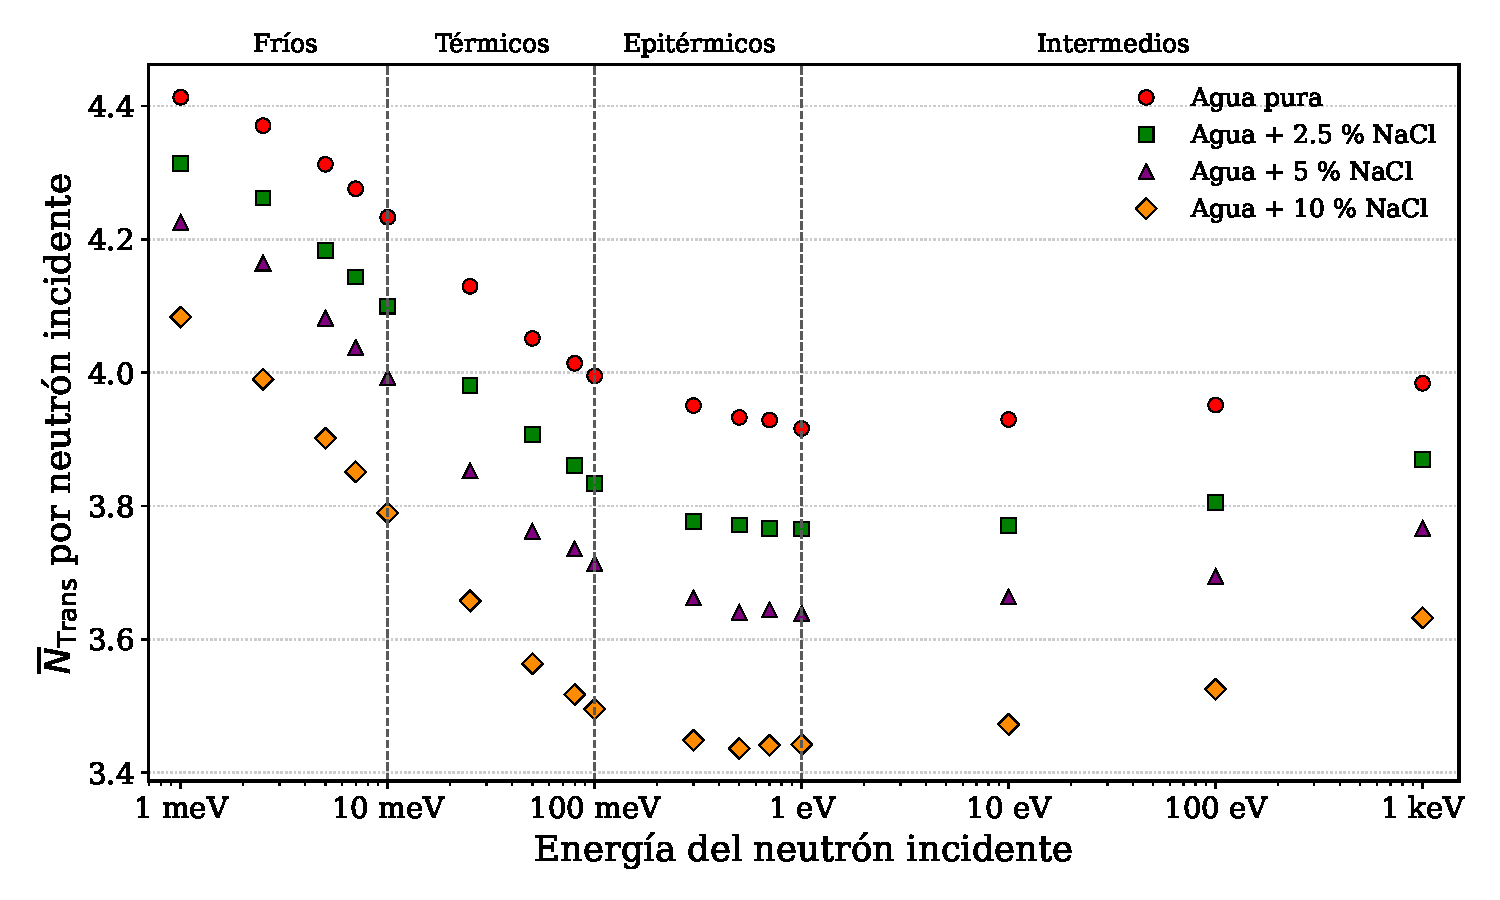
\includegraphics[width=\linewidth]{fig_4_17_transportation.pdf}
  \caption{Número medio de pasos \var{Transportation} por neutrón incidente en función de la energía (Figura~4.17 de la tesis). Las líneas verticales discontinuas separan los regímenes frío, térmico, epitérmico e intermedio.}
  \label{fig:transporte}
\end{figure}

$\overline{N}_\mathrm{Trans}$ disminuye desde el régimen frío (4.41 a 1~meV en agua pura) hasta la región de 100~meV--1~eV (3.92 a 1~eV) y vuelve a aumentar ligeramente hacia 1~keV (3.98). El NaCl lo reduce de forma sistemática (de 4.41 a 4.08 a 1~meV con 10~\% de NaCl), lo que es compatible con una terminación más temprana de parte de las historias por la mayor captura. Este observable se usa solo como control computacional; la discusión física se apoya en \var{hadElastic}, \var{nCapture} y el balance de destinos.

\subsection{Dispersión elástica}

\begin{figure}[H]
  \centering
  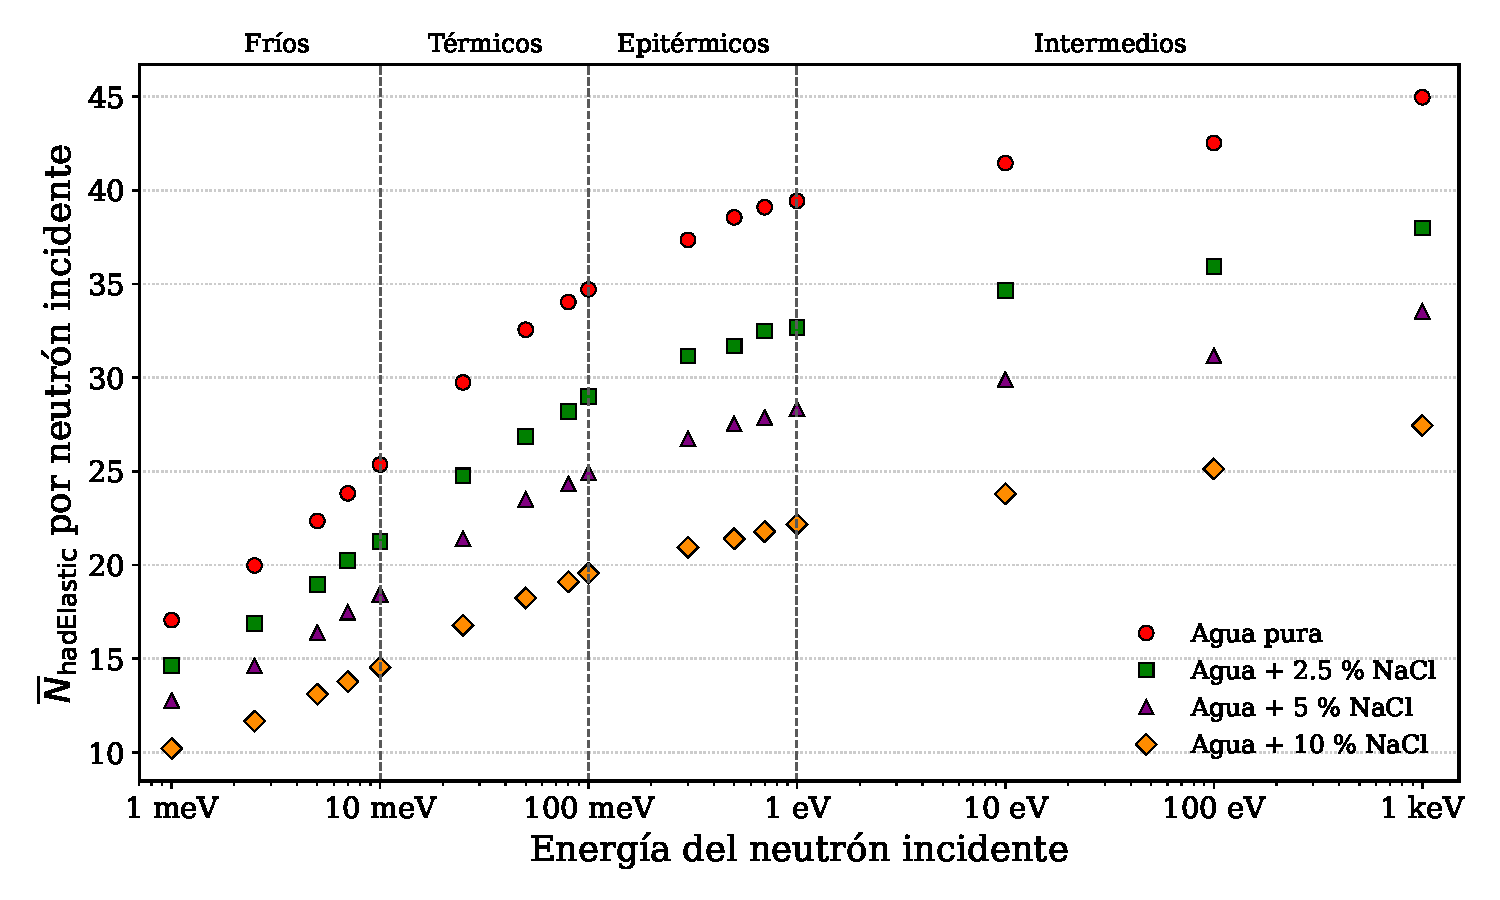
\includegraphics[width=\linewidth]{fig_4_18_hadElastic.pdf}
  \caption{Número medio de dispersiones elásticas (\var{hadElastic}) por neutrón incidente en función de la energía, para los cuatro medios (Figura~4.18 de la tesis).}
  \label{fig:hadelastic}
\end{figure}

El número medio de dispersiones elásticas por neutrón incidente aumenta con la energía, porque un neutrón más energético debe perder más letargía antes de alcanzar las energías donde la captura es probable (Figura~\ref{fig:hadelastic}). En agua pura pasa por 17.1, 25.4, 34.7, 39.4 y 45.0 a 1~meV, 10~meV, 100~meV, 1~eV y 1~keV. Con NaCl disminuye: a 1~meV, 14.6, 12.8 y 10.2 con 2.5, 5 y 10~\%, y a 1~keV, 38.0, 33.5 y 27.5. Estos promedios mezclan historias con destinos y duraciones distintos y no equivalen al número de colisiones de una historia capturada (Sección~\ref{sec:N-resultados}).

La disminución con el NaCl no se debe a una ``mejor moderación'': por colisión, el hidrógeno es el moderador más eficaz, y el Na y el Cl lo son menos. Es compatible con dos efectos simultáneos, la menor densidad de hidrógeno (Tabla~\ref{tab:medios}) y, sobre todo, el truncamiento de las historias cuando el $^{35}$Cl captura el neutrón antes de que acumule más dispersiones.

\begin{table}[H]
\centering
\small
\caption{Número medio de pasos \var{Transportation} y de dispersiones \var{hadElastic} por neutrón incidente (todas las historias).}
\label{tab:pasos}
\begin{tabular}{@{}lrrrrrrrr@{}}
\toprule
& \multicolumn{4}{c}{$\overline{N}_\mathrm{Trans}$} & \multicolumn{4}{c}{$\overline{N}_\mathrm{hadElastic}$} \\
\cmidrule(lr){2-5}\cmidrule(l){6-9}
$E$ & AP & 2.5~\% & 5~\% & 10~\% & AP & 2.5~\% & 5~\% & 10~\% \\
\midrule
\csname @@input\endcsname figuras-procesamiento-64-corridas/tabla_pasos.tex
\bottomrule
\end{tabular}
\end{table}

% =====================================================================
\section{Moderación}
\label{sec:moderacion}

\subsection{Número de dispersiones elásticas antes de la captura}
\label{sec:N-resultados}

El número de dispersiones elásticas que experimenta un neutrón antes de ser capturado caracteriza su historia de moderación dentro del detector. La Figura~\ref{fig:N-AP} muestra las distribuciones $P(N\mid\text{captura})$ en agua pura y la Figura~\ref{fig:N-NaCl}, las de los medios con NaCl.

\begin{figure}[H]
  \centering
  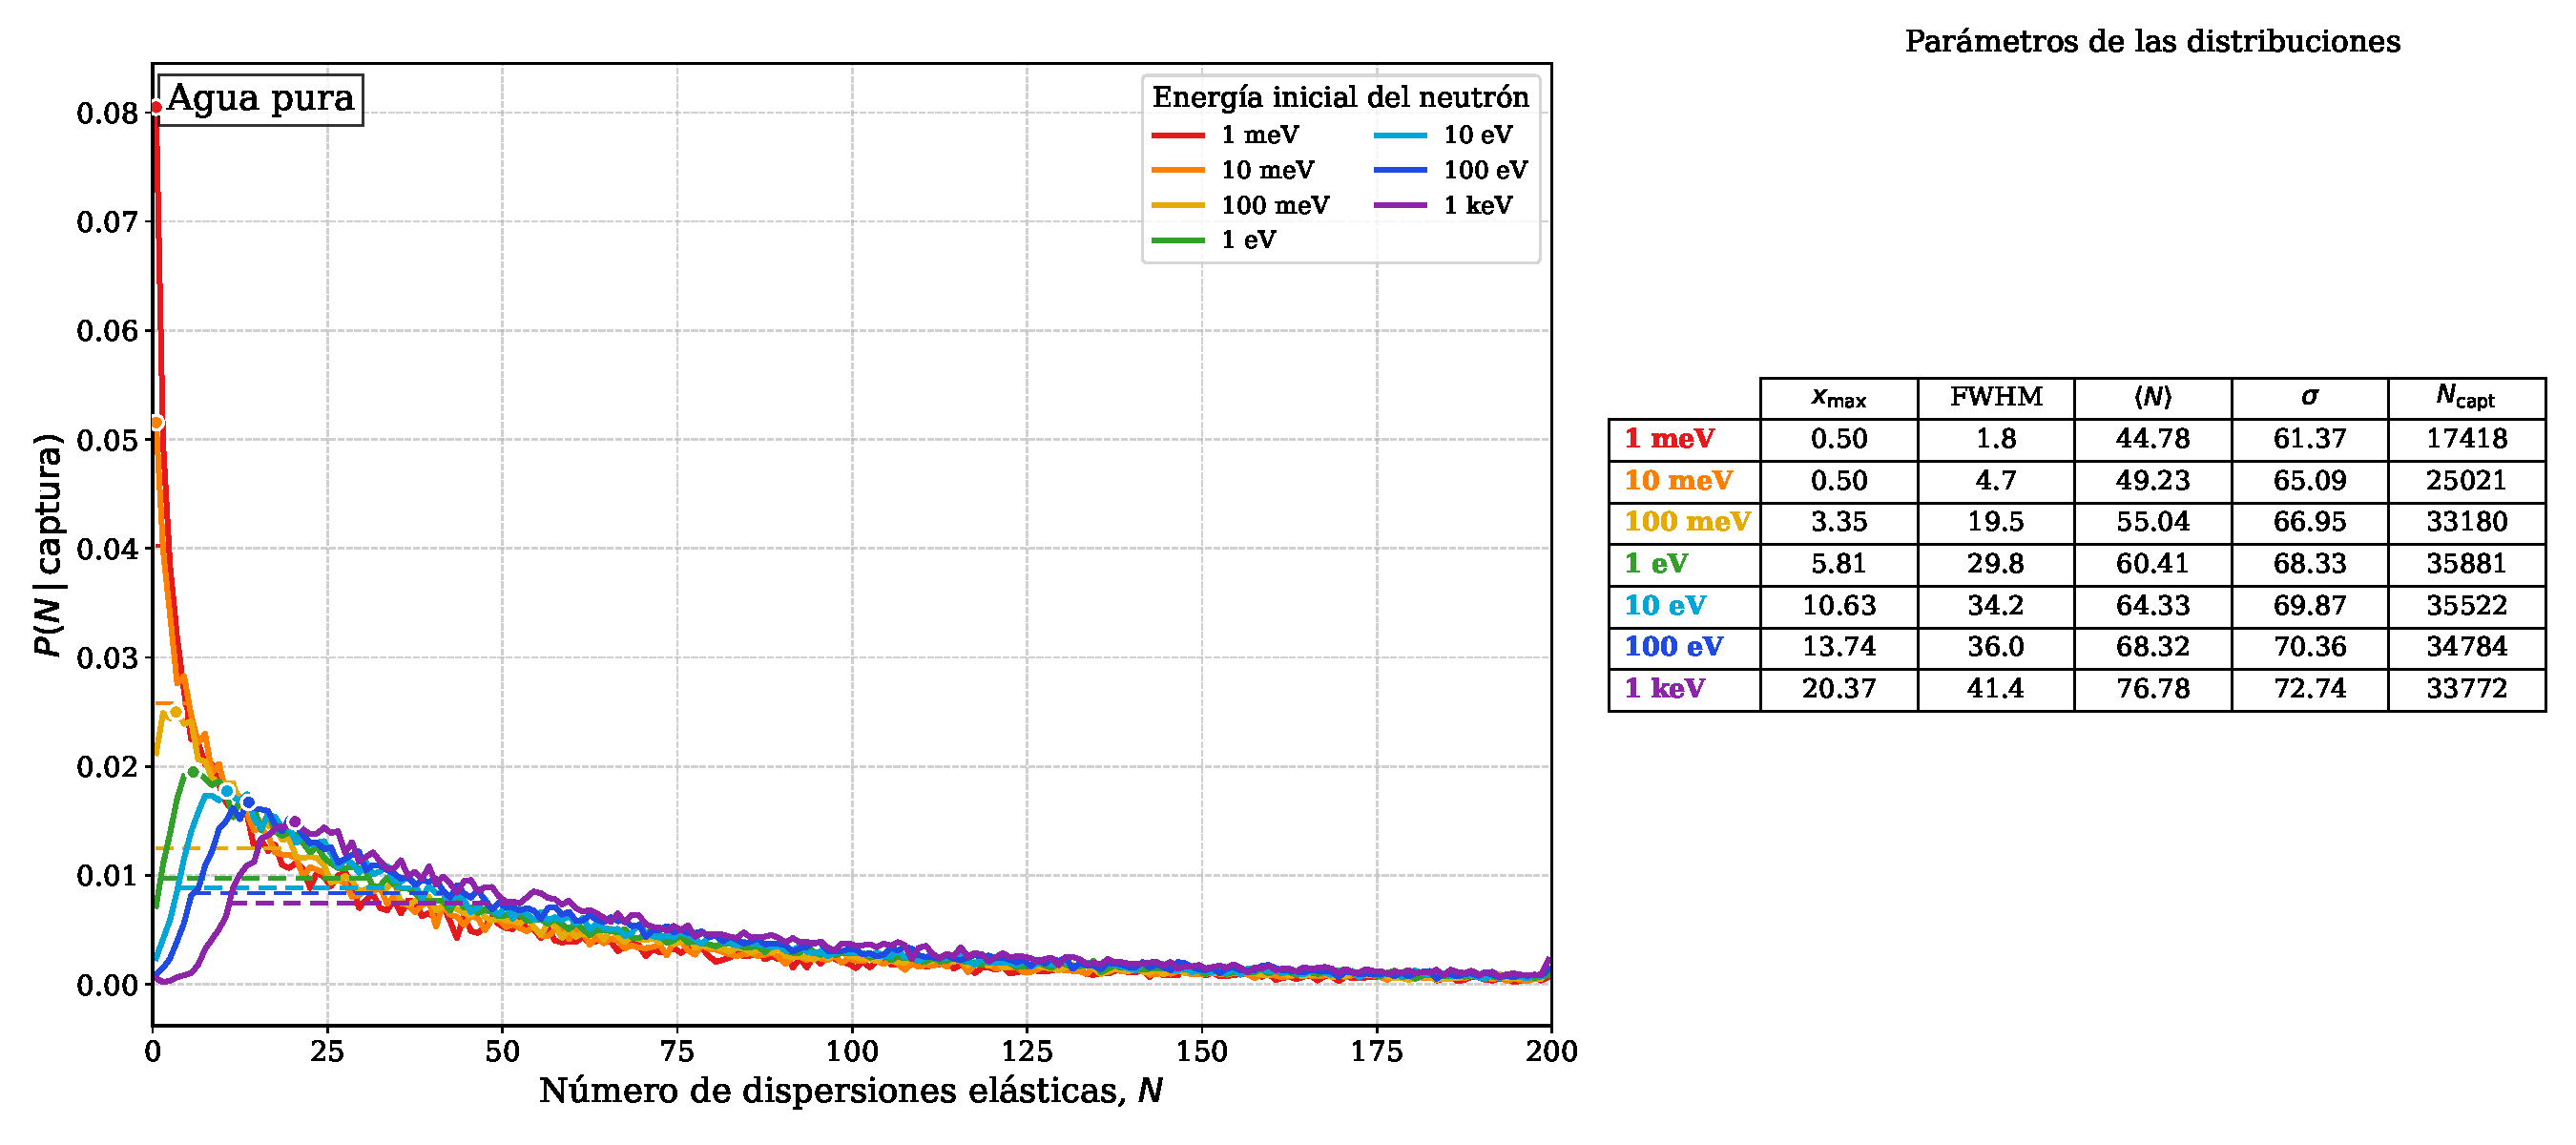
\includegraphics[width=\linewidth]{fig_4_19_N_agua_pura.pdf}
  \caption{Distribuciones normalizadas $P(N\mid\text{captura})$ del número de dispersiones elásticas antes de la captura en agua pura, para siete energías entre 1~meV y 1~keV (Figura~4.19 de la tesis). La tabla da la posición del máximo, la FWHM, la media, la desviación estándar y el número de capturas.}
  \label{fig:N-AP}
\end{figure}

A 1~meV la distribución tiene su máximo prácticamente en $N\simeq0$: una fracción importante de los neutrones fríos se captura casi sin moderarse. Al aumentar la energía, el máximo se desplaza a valores mayores y la distribución se ensancha: $x_\mathrm{max}$ pasa de 0.5 a 20.4 dispersiones y la FWHM de 1.8 a 41.4 entre 1~meV y 1~keV, y $\langle N\rangle$ de 44.78 a 76.78. Para $N\gtrsim100$, todas las distribuciones tienen colas muy similares, compatibles con una pérdida de memoria de la energía inicial.

\begin{figure}[H]
  \centering
  \includegraphics[width=\linewidth]{{fig_D_1_N_2.5NaCl}.pdf}\\[0.3em]
  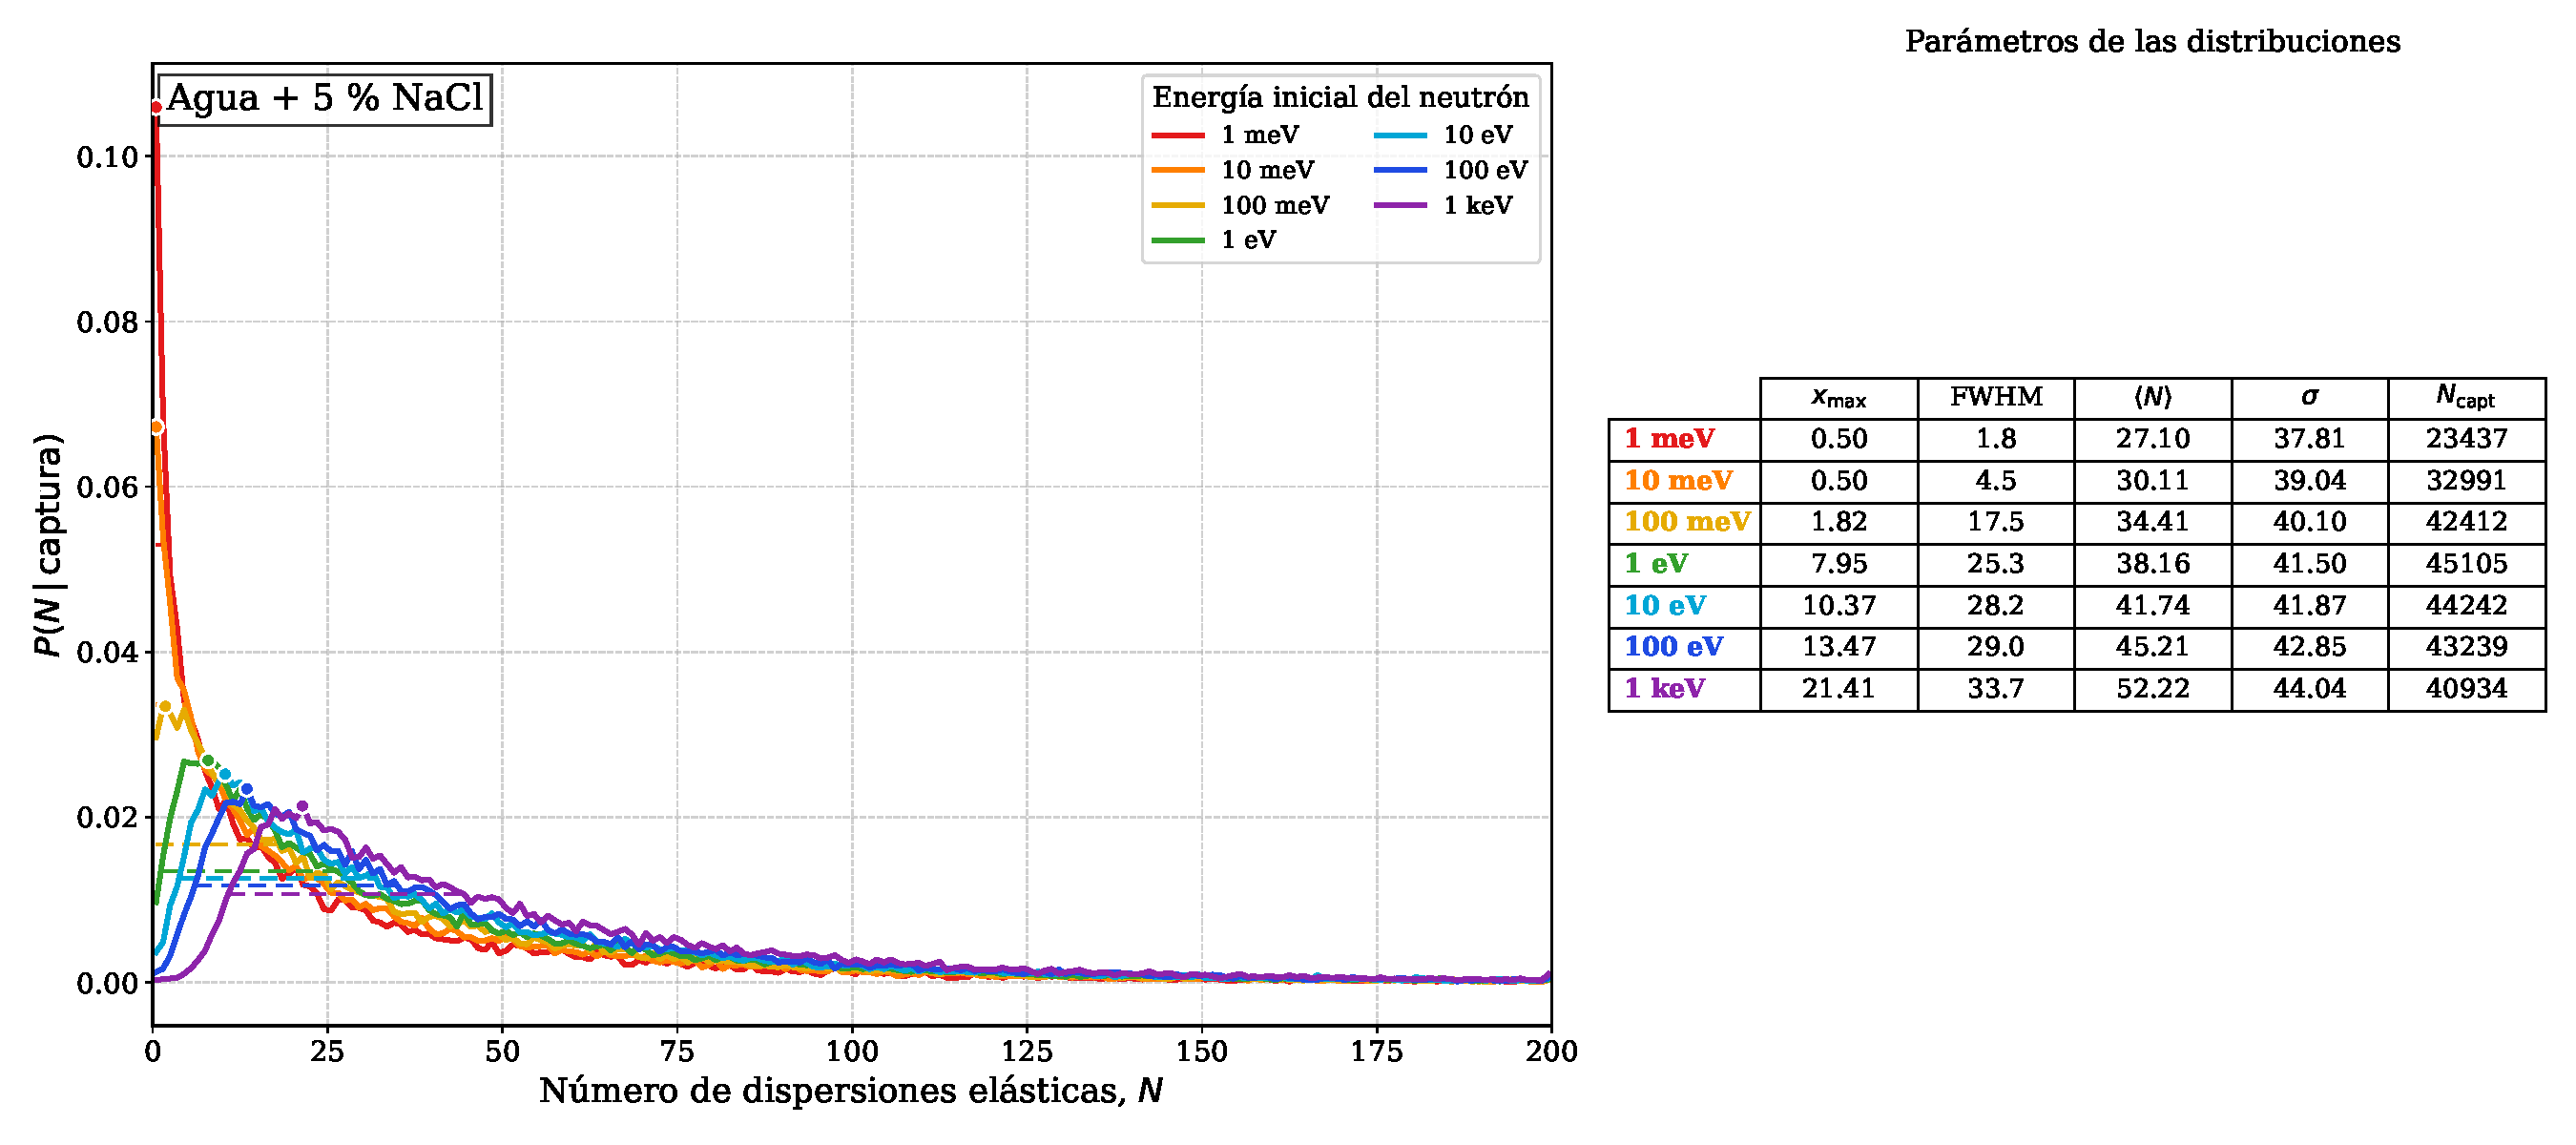
\includegraphics[width=\linewidth]{fig_D_2_N_5NaCl.pdf}\\[0.3em]
  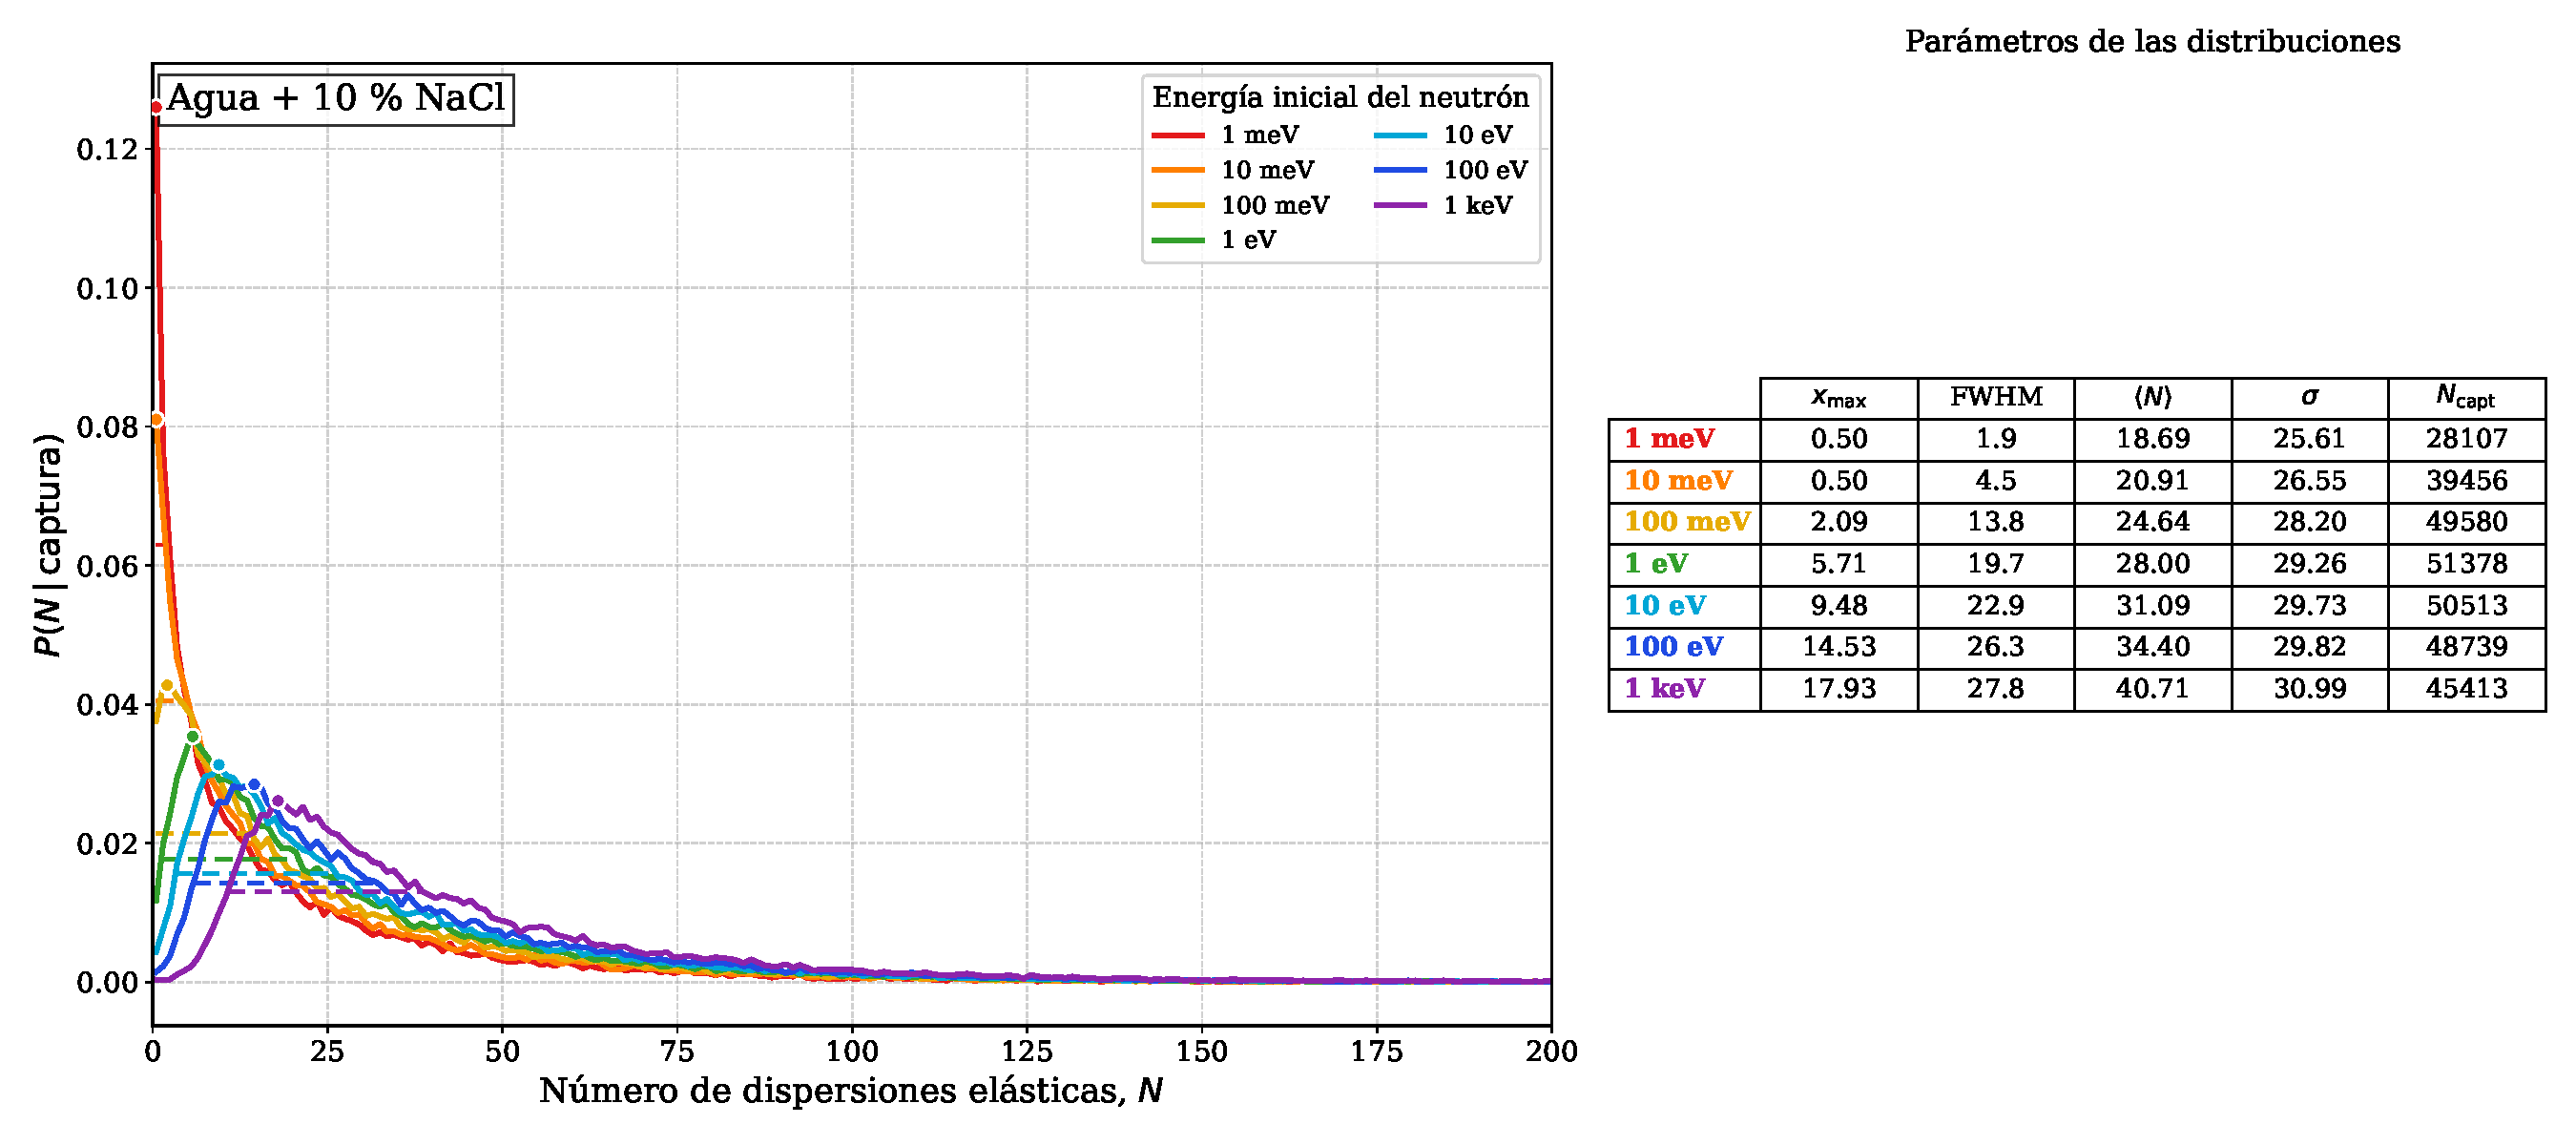
\includegraphics[width=\linewidth]{fig_D_3_N_10NaCl.pdf}
  \caption{$P(N\mid\text{captura})$ en agua con 2.5, 5 y 10~\% de NaCl (Figuras~D.1--D.3 de la tesis).}
  \label{fig:N-NaCl}
\end{figure}

\begin{figure}[H]
  \centering
  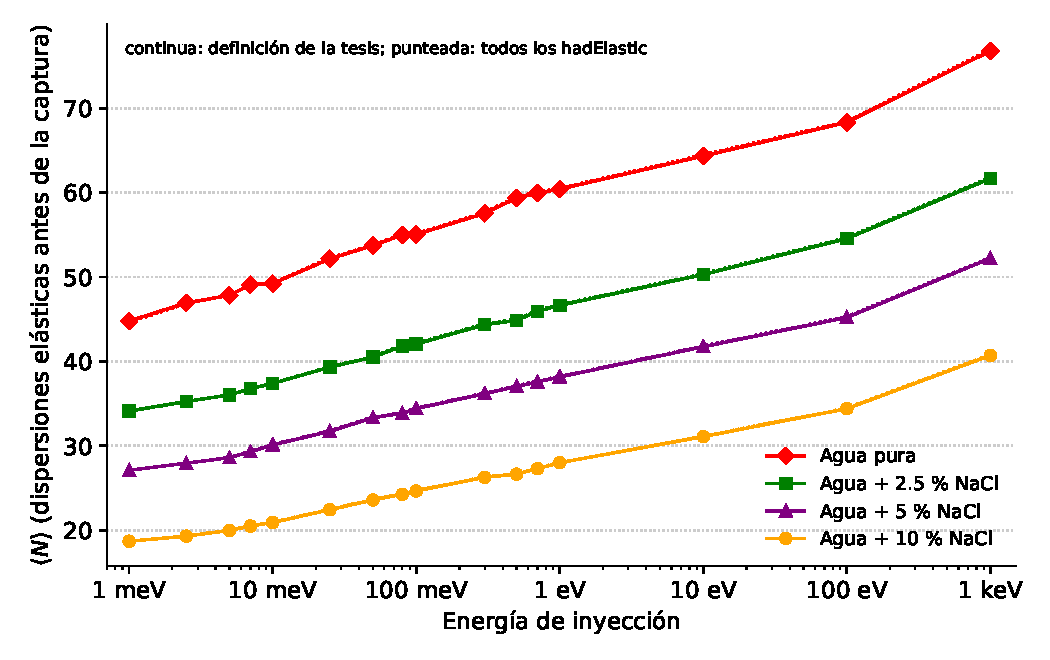
\includegraphics[width=0.78\linewidth]{N_medio.pdf}
  \caption{$\langle N\rangle$ en función de la energía de inyección para los cuatro medios. Línea continua: definición de la tesis; línea punteada: todas las dispersiones elásticas de la historia capturada. Las dos definiciones difieren en menos del 0.5~\%.}
  \label{fig:N-medio}
\end{figure}

$\langle N\rangle$ crece de forma monótona con la energía en los cuatro medios y disminuye con la concentración de NaCl (Figura~\ref{fig:N-medio}): a 1~meV pasa de 44.8 en agua pura a 34.1, 27.1 y 18.7 con 2.5, 5 y 10~\%, y a 1~keV, de 76.8 a 61.7, 52.2 y 40.7.

\textbf{Interpretación.} Las distribuciones son condicionales a la captura y no miden sin sesgo la moderación de todos los neutrones incidentes. Entre las historias capturadas, las de mayor energía inicial requieren más colisiones y son más dispersas. El NaCl aumenta la absorción, sobre todo por $^{35}$Cl, y selecciona historias que terminan antes; por eso la reducción de $N$ no demuestra que la moderación mejore ni que se mantenga igual. La conclusión sustentada es que el dopante modifica claramente la competencia entre captura y escape, mientras que el hidrógeno conserva el papel dominante en la pérdida de energía por colisión.

\subsection{Letargía por colisión, $\xi$}
\label{sec:xi-resultados}

La energía térmica del medio a 20~$^\circ$C es $k_BT\simeq25.3$~meV, y la energía cinética media de un núcleo, $\tfrac32k_BT\simeq37.9$~meV~\cite{Callen1985}. Según la relación entre la energía del neutrón y esta escala, la distribución de $\xi$ cambia de comportamiento. En las tablas de esta sección se dan $\langle\xi\rangle$ y $\sigma(\xi)$ para los cuatro medios; las figuras de agua pura corresponden a las de la tesis y las de los medios con NaCl están en las Figuras~\ref{fig:xi-fria-NaCl} y en el Apéndice~\ref{ap:xi}.

\subsubsection{Régimen frío (1--10~meV)}

\begin{figure}[H]
  \centering
  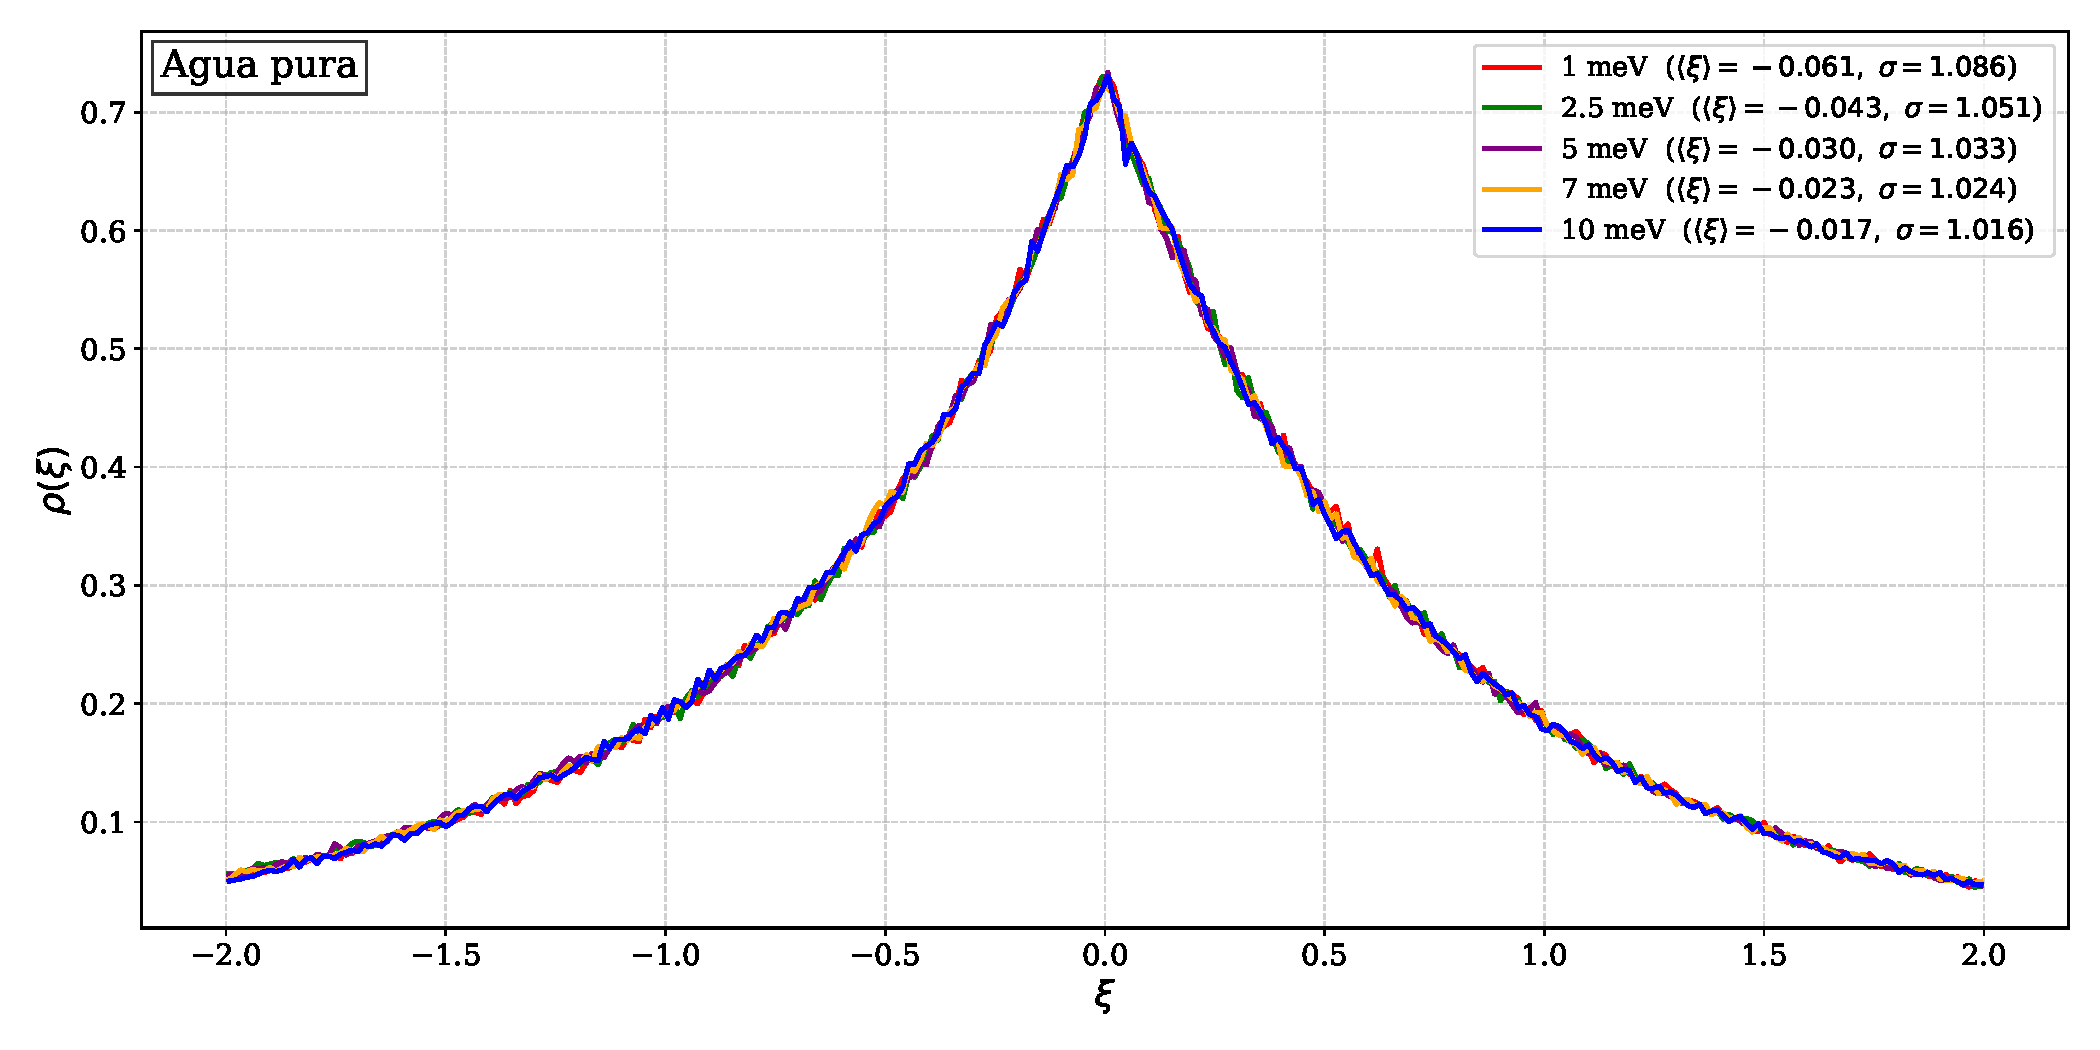
\includegraphics[width=0.92\linewidth]{fig_4_20_xi_AP_fria.pdf}
  \caption{Distribución de $\xi$ en agua pura para 1, 2.5, 5, 7 y 10~meV, normalizada a área unitaria (Figura~4.20 de la tesis).}
  \label{fig:xi-fria}
\end{figure}

En este régimen, la energía del neutrón es menor que la energía térmica del medio. Las distribuciones tienen medias negativas, sobre todo a 1 y 2.5~meV: en promedio, el neutrón gana energía de los núcleos en movimiento térmico. Al aumentar la energía, $\langle\xi\rangle$ se acerca a cero y $\sigma(\xi)$ disminuye (de 1.086 a 1.016 en agua pura), porque el neutrón se acerca al equilibrio térmico y las ganancias y pérdidas se compensan. Con NaCl, $\langle\xi\rangle$ es más negativo (de $-0.061$ en agua pura a $-0.137$ con 10~\% a 1~meV). Este corrimiento es compatible con la dispersión térmica y con la selección de historias más cortas, pero no se puede atribuir al Na o al Cl sin separar la distribución por núcleo dispersor.

\begin{table}[H]
\centering
\small
\caption{$\langle\xi\rangle$ y $\sigma(\xi)$ en el régimen frío.}
\label{tab:xi-fria}
\begin{tabular}{@{}lrrrrrrrr@{}}
\toprule
& \multicolumn{2}{c}{Agua pura} & \multicolumn{2}{c}{2.5~\% NaCl} & \multicolumn{2}{c}{5~\% NaCl} & \multicolumn{2}{c}{10~\% NaCl} \\
\cmidrule(lr){2-3}\cmidrule(lr){4-5}\cmidrule(lr){6-7}\cmidrule(l){8-9}
$E$ & $\langle\xi\rangle$ & $\sigma$ & $\langle\xi\rangle$ & $\sigma$ & $\langle\xi\rangle$ & $\sigma$ & $\langle\xi\rangle$ & $\sigma$ \\
\midrule
\csname @@input\endcsname figuras-procesamiento-64-corridas/tabla_xi_fria.tex
\bottomrule
\end{tabular}
\end{table}

\begin{figure}[H]
  \centering
  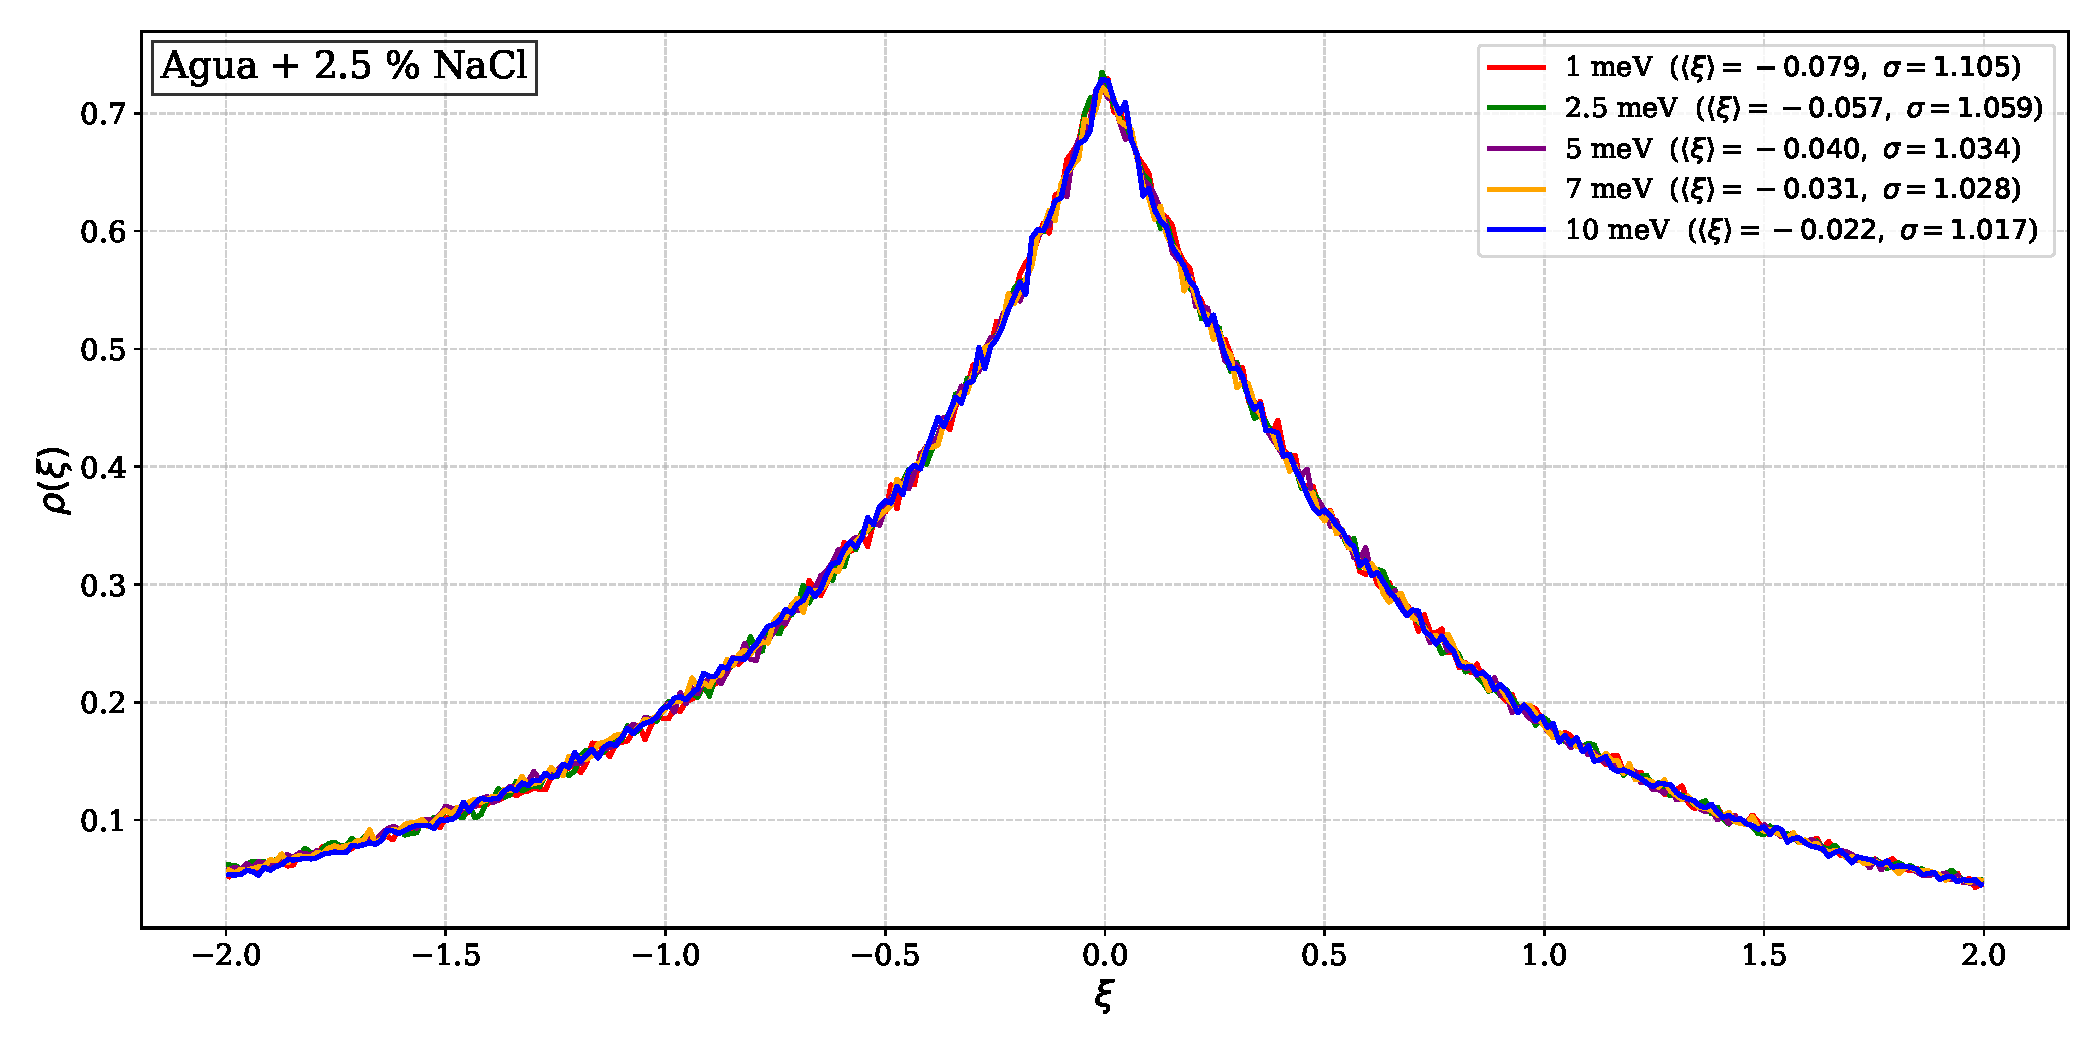
\includegraphics[width=0.78\linewidth]{fig_D_4_xi_A25NaCl_fria.pdf}\\[0.2em]
  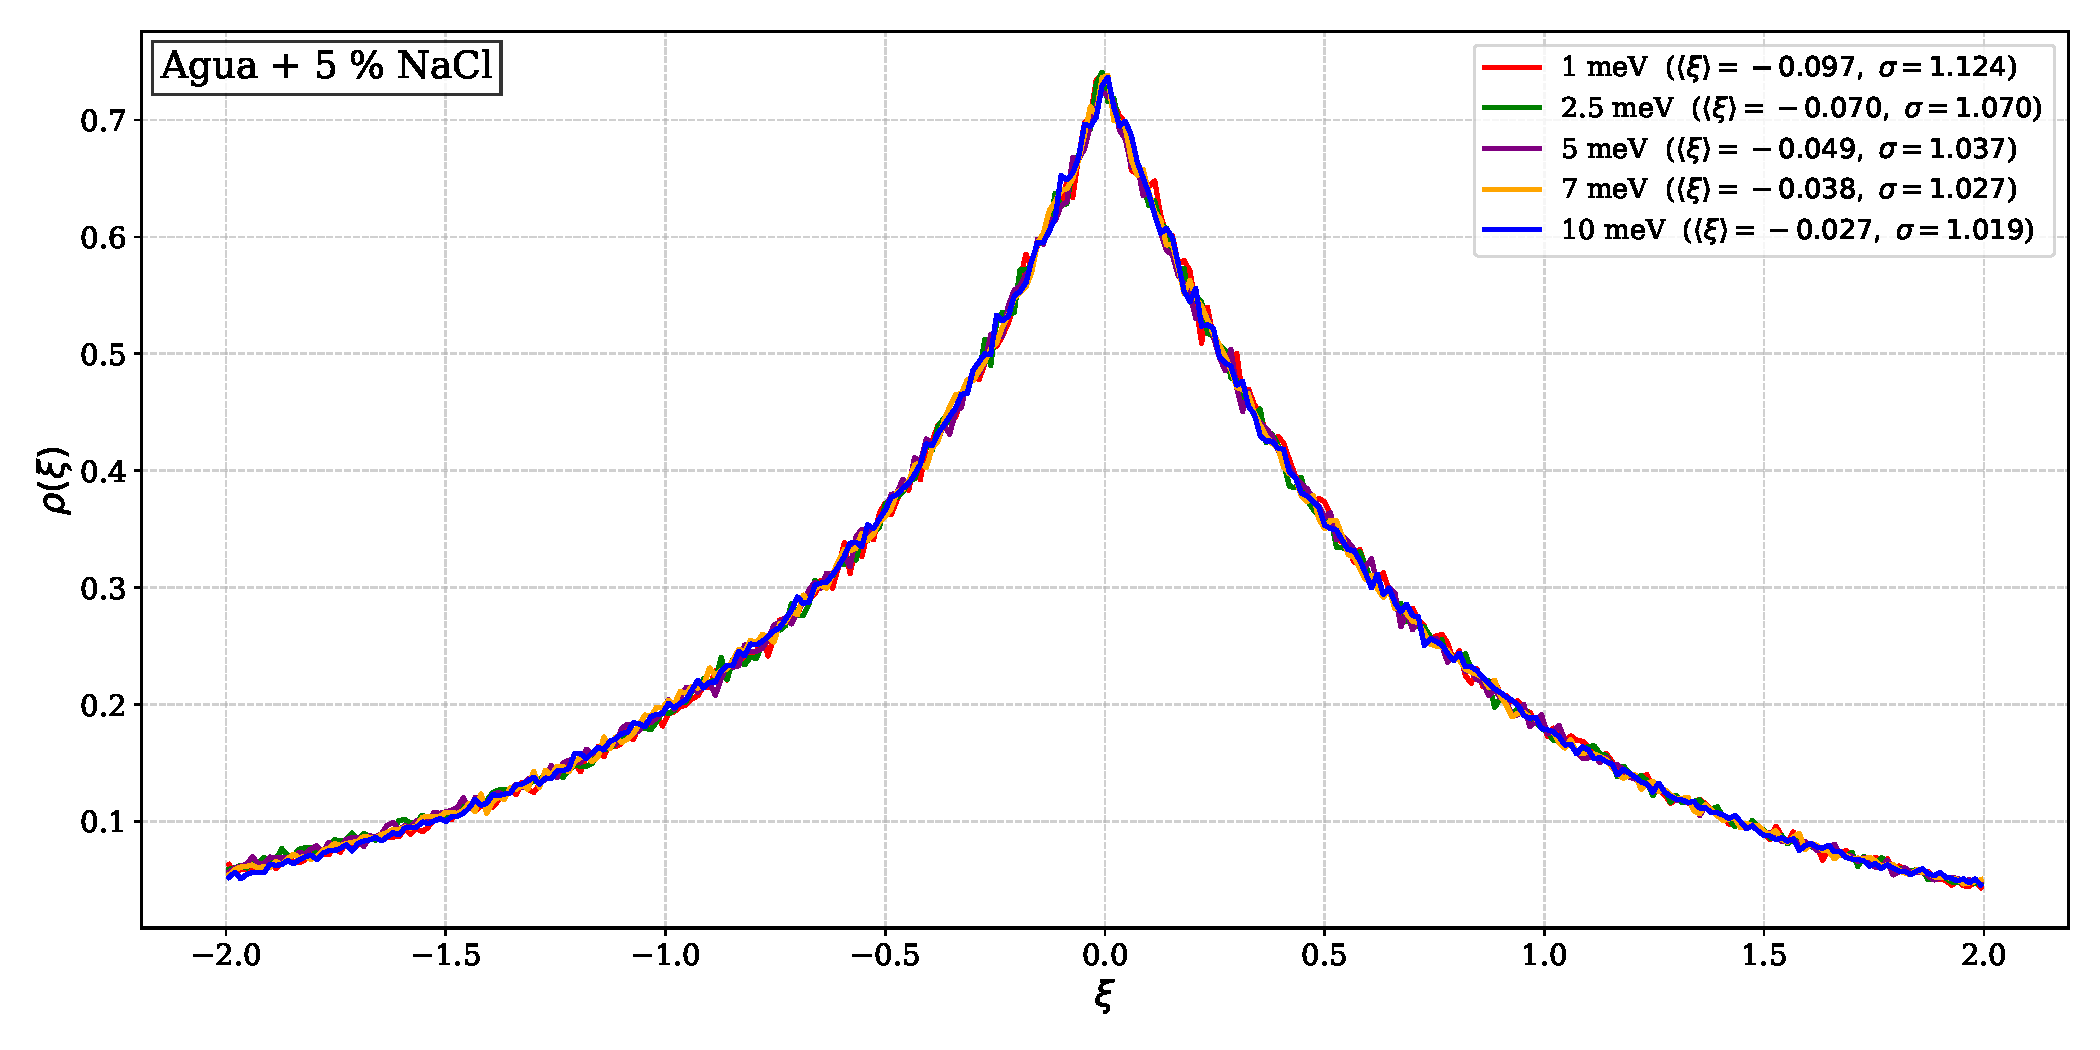
\includegraphics[width=0.78\linewidth]{fig_D_5_xi_A5NaCl_fria.pdf}\\[0.2em]
  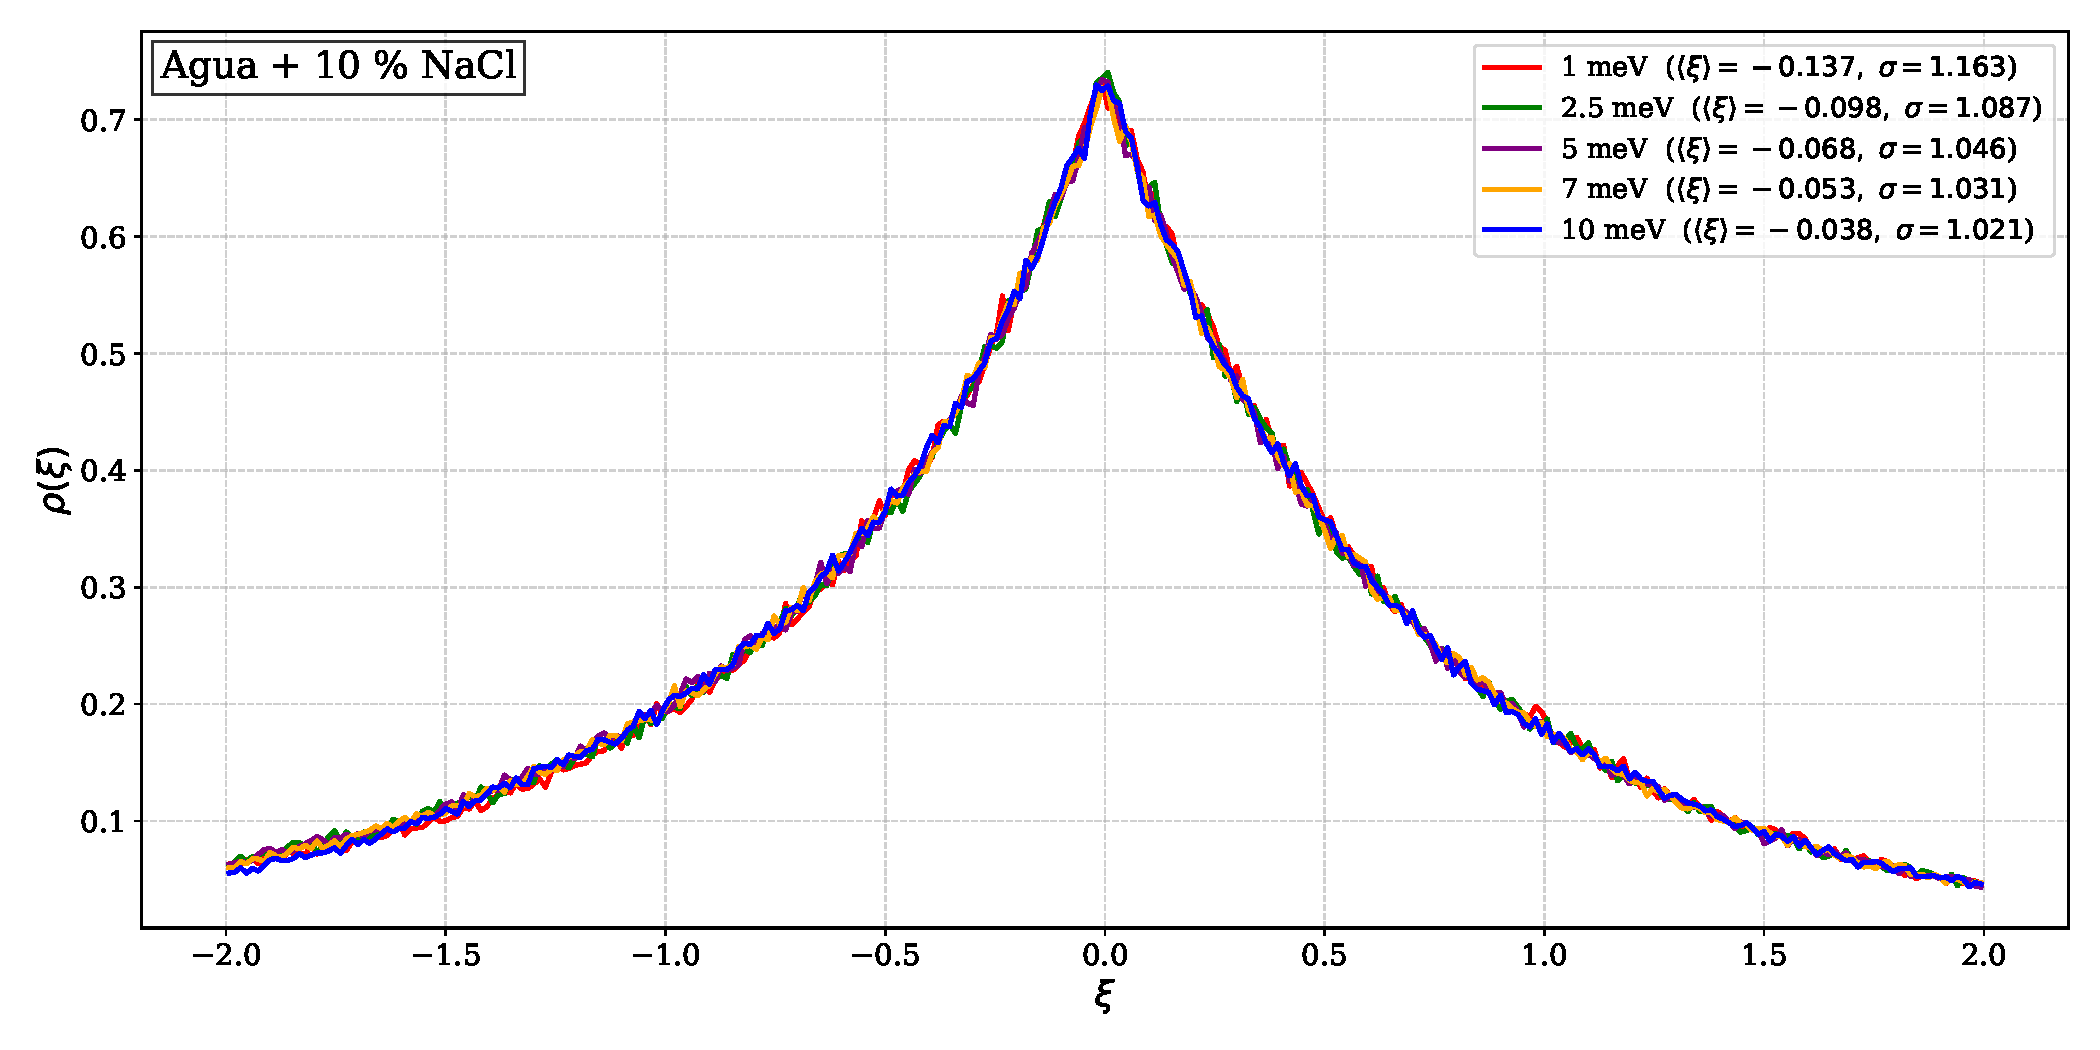
\includegraphics[width=0.78\linewidth]{fig_D_6_xi_A10NaCl_fria.pdf}
  \caption{Distribución de $\xi$ en el régimen frío para agua con 2.5, 5 y 10~\% de NaCl (Figuras~D.4--D.6 de la tesis).}
  \label{fig:xi-fria-NaCl}
\end{figure}

\subsubsection{Régimen térmico (10--100~meV)}

\begin{figure}[H]
  \centering
  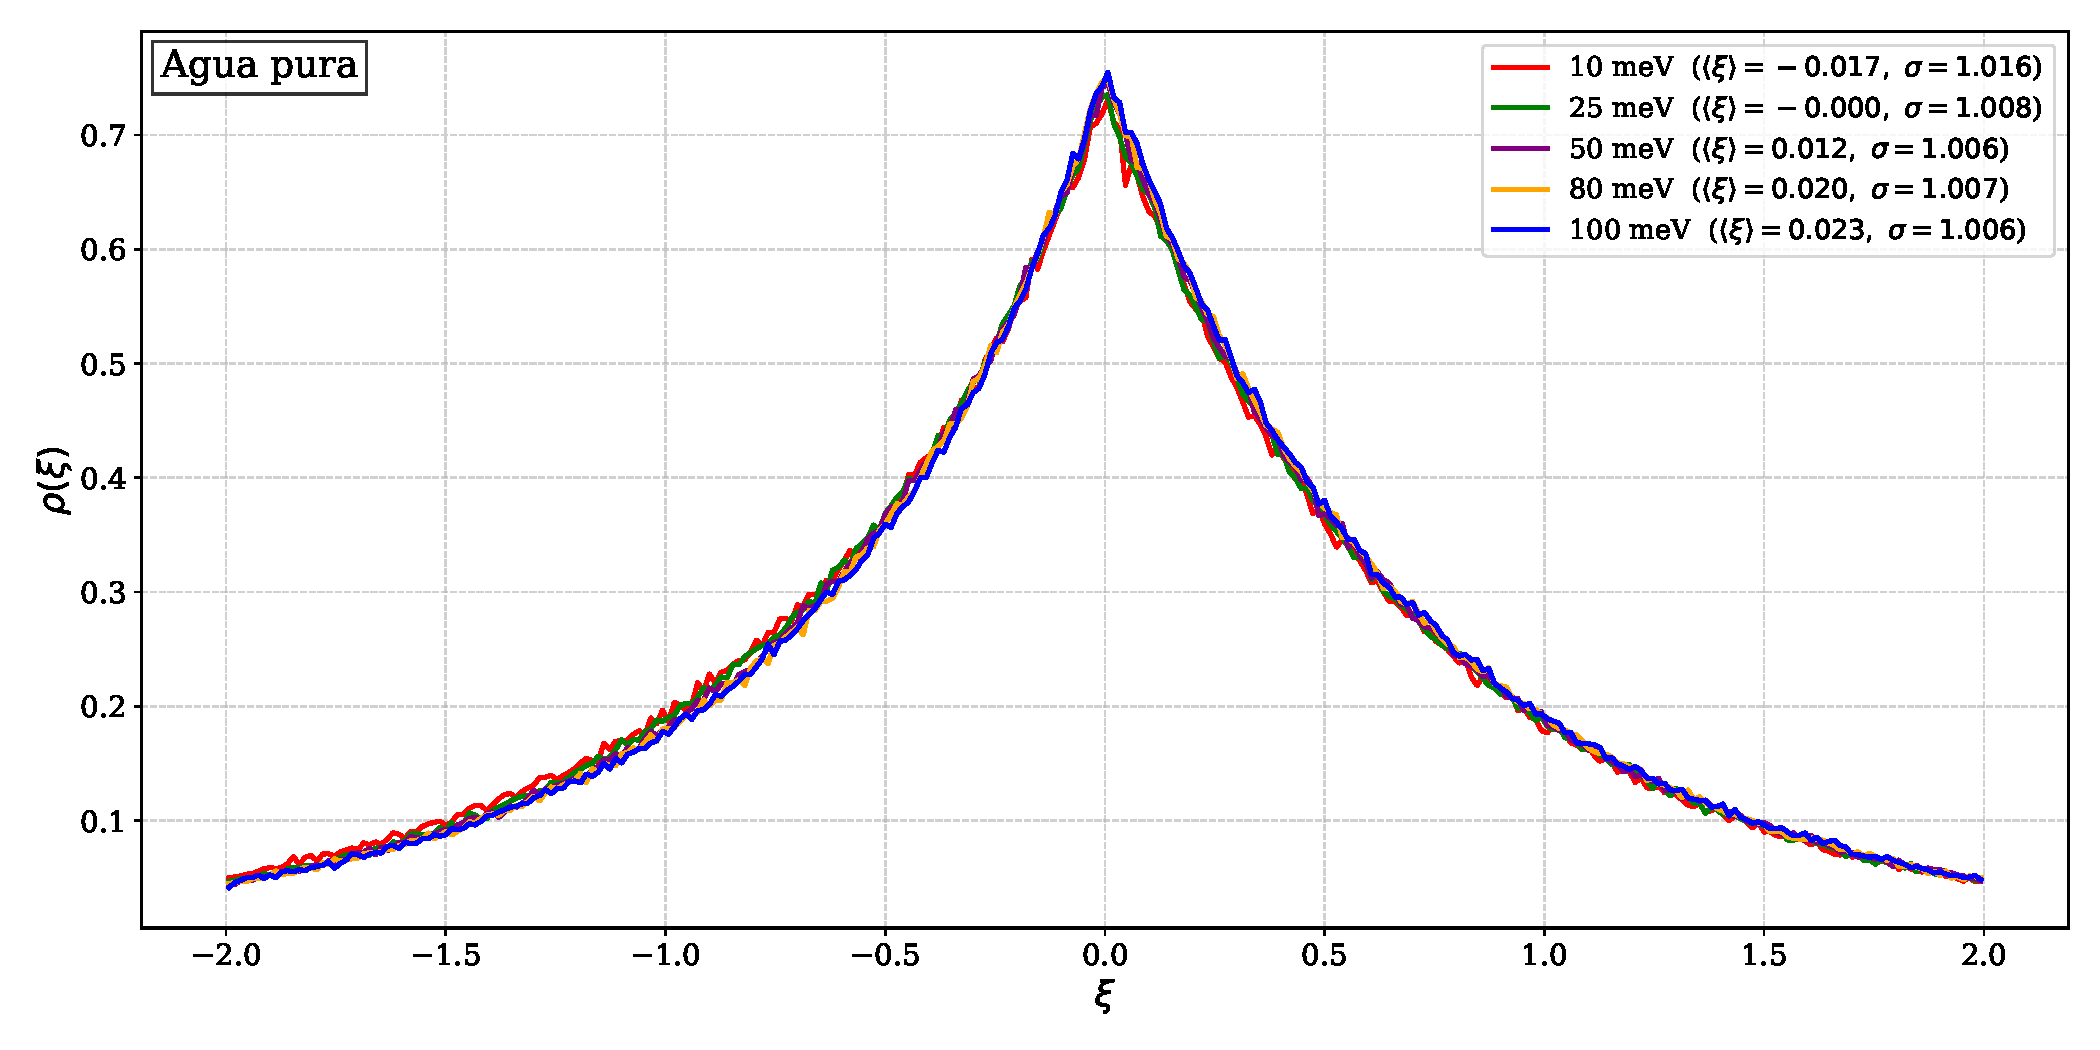
\includegraphics[width=0.92\linewidth]{fig_4_21_xi_AP_termica.pdf}
  \caption{Distribución de $\xi$ en agua pura para 10, 25, 50, 80 y 100~meV (Figura~4.21 de la tesis).}
  \label{fig:xi-termica}
\end{figure}

Las distribuciones son aproximadamente simétricas alrededor de $\xi\simeq0$, con $\sigma(\xi)\simeq1$: la energía del neutrón es comparable a $k_BT$ y las colisiones elásticas producen tanto pérdidas como ganancias de energía. $\langle\xi\rangle$ es ligeramente negativo a 10~meV ($-0.017$ en agua pura), prácticamente nulo a 25~meV ($-0.0001$, la energía térmica) y positivo a partir de 50~meV (0.023 a 100~meV): la pérdida de energía empieza a dominar. En este régimen, $\xi$ depende débilmente de la energía inicial y de la composición.

\begin{table}[H]
\centering
\small
\caption{$\langle\xi\rangle$ y $\sigma(\xi)$ en el régimen térmico.}
\label{tab:xi-termica}
\begin{tabular}{@{}lrrrrrrrr@{}}
\toprule
& \multicolumn{2}{c}{Agua pura} & \multicolumn{2}{c}{2.5~\% NaCl} & \multicolumn{2}{c}{5~\% NaCl} & \multicolumn{2}{c}{10~\% NaCl} \\
\cmidrule(lr){2-3}\cmidrule(lr){4-5}\cmidrule(lr){6-7}\cmidrule(l){8-9}
$E$ & $\langle\xi\rangle$ & $\sigma$ & $\langle\xi\rangle$ & $\sigma$ & $\langle\xi\rangle$ & $\sigma$ & $\langle\xi\rangle$ & $\sigma$ \\
\midrule
\csname @@input\endcsname figuras-procesamiento-64-corridas/tabla_xi_termica.tex
\bottomrule
\end{tabular}
\end{table}

\subsubsection{Régimen epitérmico (100~meV--1~eV)}

\begin{figure}[H]
  \centering
  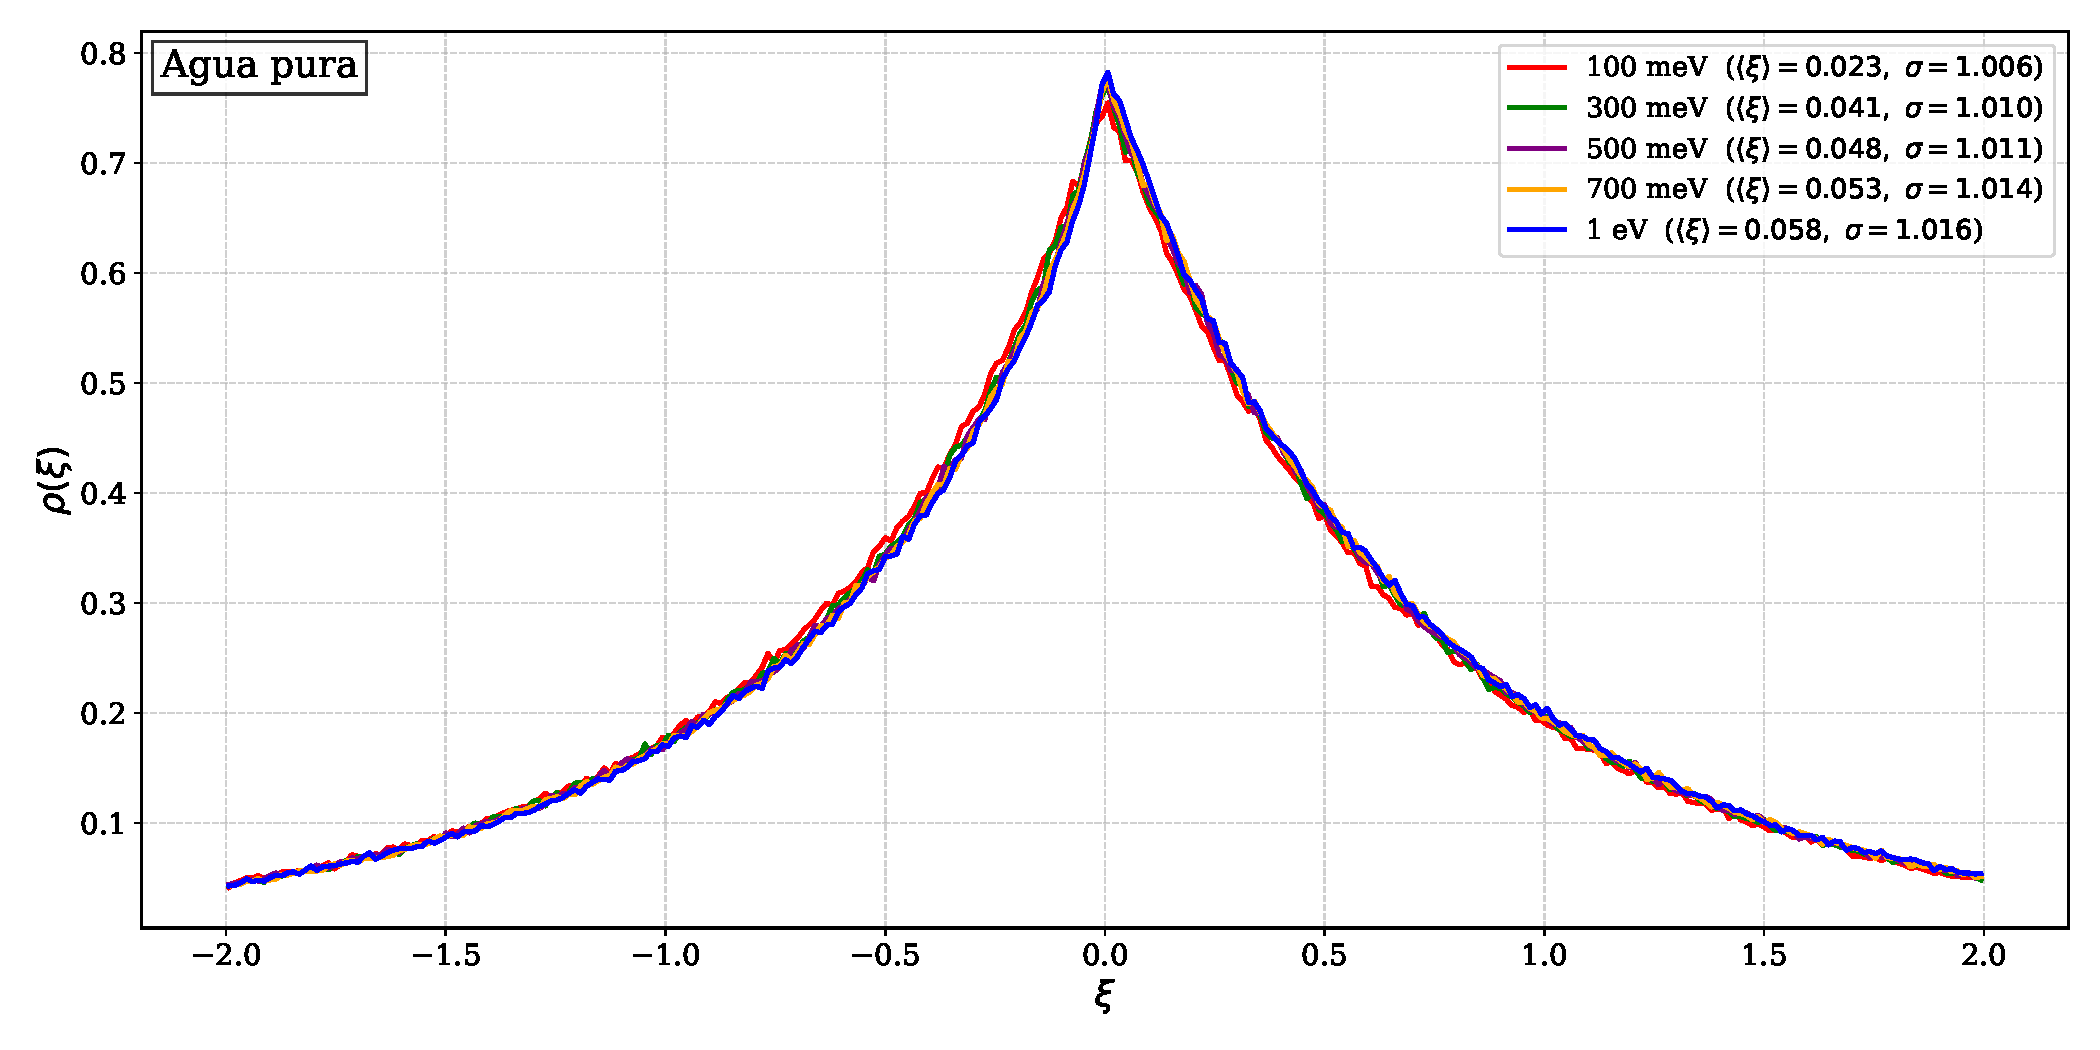
\includegraphics[width=0.92\linewidth]{fig_4_22_xi_AP_epitermica.pdf}
  \caption{Distribución de $\xi$ en agua pura para 100, 300, 500 y 700~meV y 1~eV (Figura~4.22 de la tesis).}
  \label{fig:xi-epitermica}
\end{figure}

Todas las distribuciones están centradas en $\xi>0$ y $\langle\xi\rangle$ crece con la energía (de 0.023 a 0.058 en agua pura): la transferencia neta de energía va del neutrón al medio (\textit{down-scattering}), como se espera cuando $E_n$ deja de ser comparable con $k_BT$. $\sigma(\xi)$ permanece cerca de la unidad. El aumento de $\langle\xi\rangle$ con la salinidad caracteriza la muestra de colisiones de neutrones que después se capturan; no representa el decremento elemental del Na o del Cl ni una mayor pérdida de energía por colisión, ya que para un blanco libre el decremento medio disminuye con la masa nuclear.

\begin{table}[H]
\centering
\small
\caption{$\langle\xi\rangle$ y $\sigma(\xi)$ en el régimen epitérmico.}
\label{tab:xi-epitermica}
\begin{tabular}{@{}lrrrrrrrr@{}}
\toprule
& \multicolumn{2}{c}{Agua pura} & \multicolumn{2}{c}{2.5~\% NaCl} & \multicolumn{2}{c}{5~\% NaCl} & \multicolumn{2}{c}{10~\% NaCl} \\
\cmidrule(lr){2-3}\cmidrule(lr){4-5}\cmidrule(lr){6-7}\cmidrule(l){8-9}
$E$ & $\langle\xi\rangle$ & $\sigma$ & $\langle\xi\rangle$ & $\sigma$ & $\langle\xi\rangle$ & $\sigma$ & $\langle\xi\rangle$ & $\sigma$ \\
\midrule
\csname @@input\endcsname figuras-procesamiento-64-corridas/tabla_xi_epitermica.tex
\bottomrule
\end{tabular}
\end{table}

\subsubsection{Régimen intermedio (1~eV--1~keV)}

\begin{figure}[H]
  \centering
  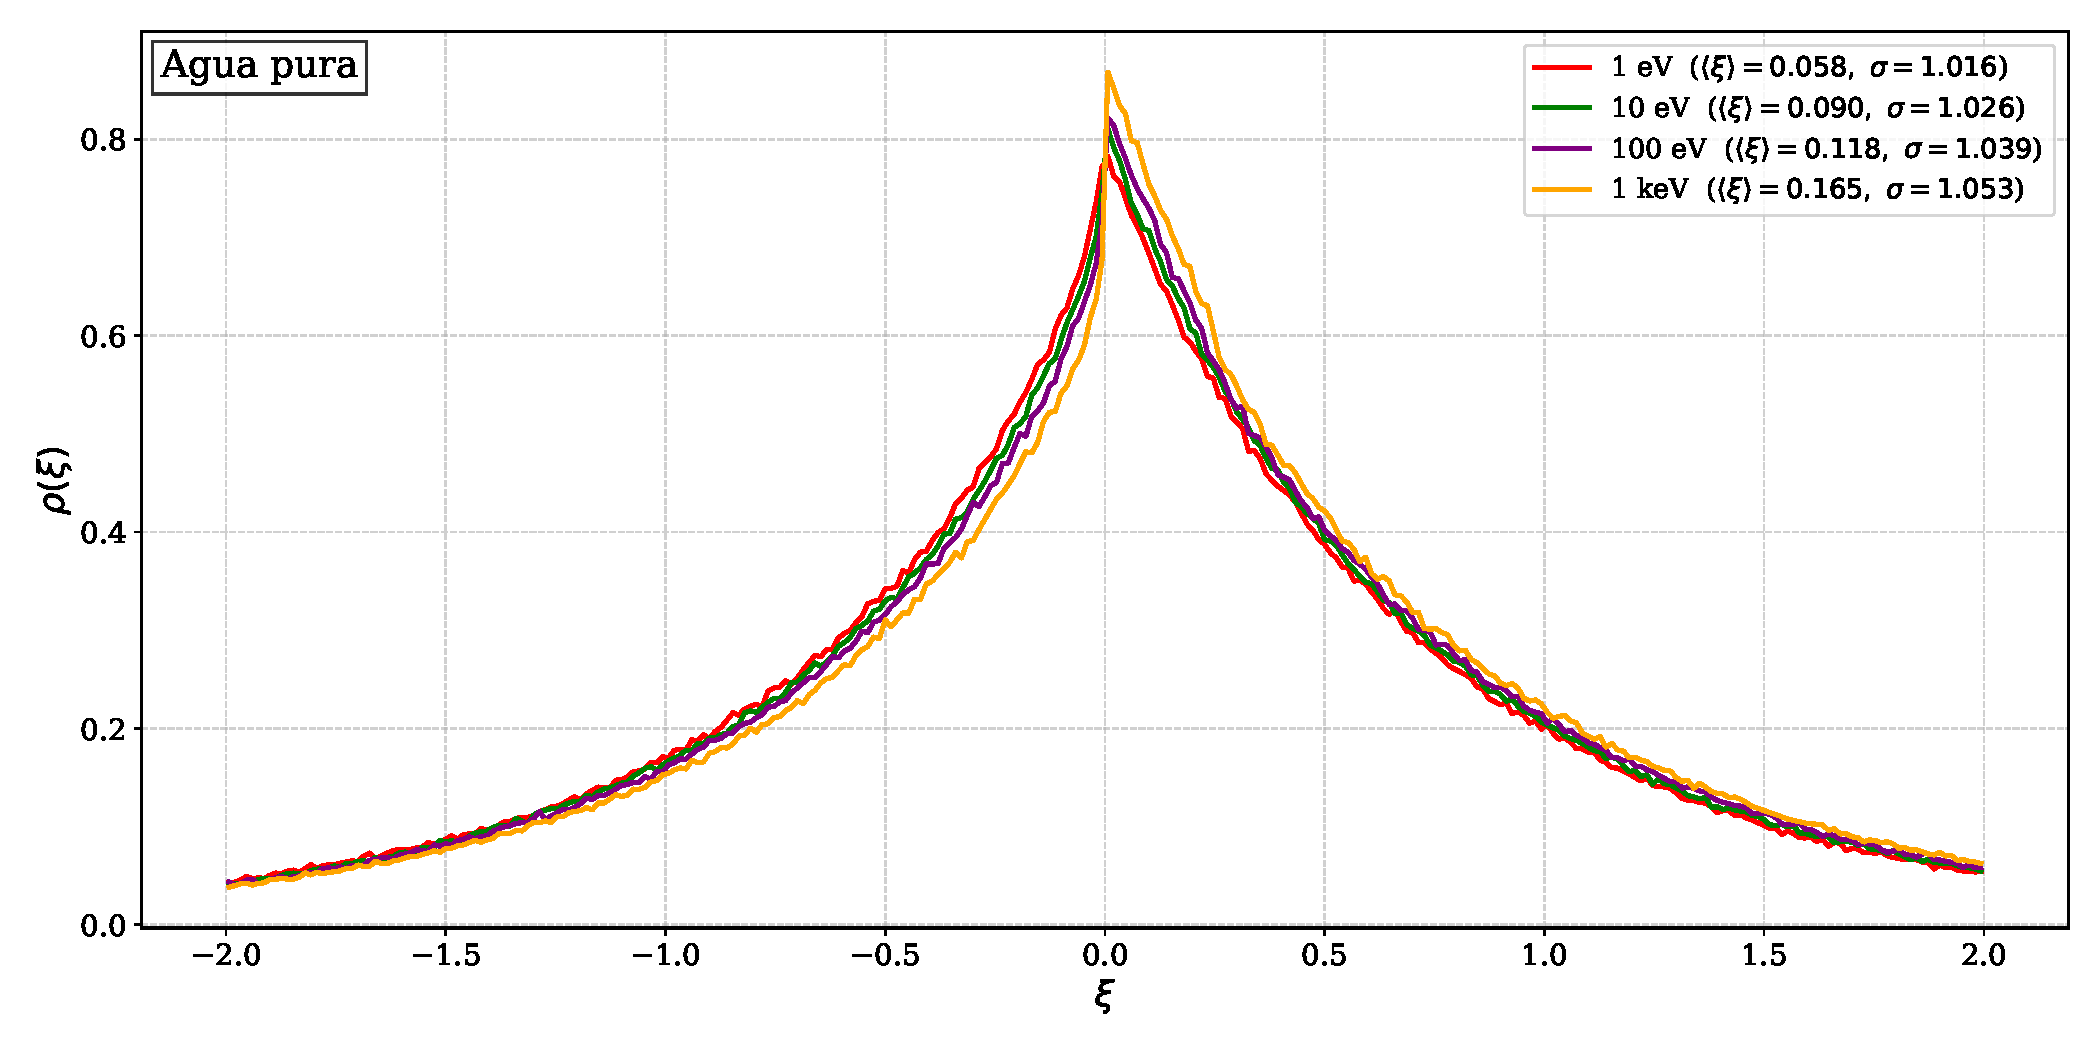
\includegraphics[width=0.92\linewidth]{fig_4_23_xi_AP_intermedia.pdf}
  \caption{Distribución de $\xi$ en agua pura para 1, 10 y 100~eV y 1~keV (Figura~4.23 de la tesis).}
  \label{fig:xi-intermedia}
\end{figure}

En agua pura, $\langle\xi\rangle$ aumenta de 0.058 a 0.165 entre 1~eV y 1~keV; con 2.5, 5 y 10~\% de NaCl, los intervalos son 0.075--0.205, 0.091--0.242 y 0.122--0.308 (Tabla~4.6 de la tesis, reproducida en la Tabla~\ref{tab:xi-intermedia}). La desviación estándar cambia muy poco ($1.009\le\sigma\le1.065$): el NaCl desplaza el valor medio pero no modifica de forma apreciable la anchura ni la forma de la distribución. Las formas semejantes indican que no aparece un mecanismo de moderación nuevo en esta región.

\begin{table}[H]
\centering
\small
\caption{$\langle\xi\rangle$ y $\sigma(\xi)$ en el régimen intermedio. Los extremos de cada columna son los valores mínimo y máximo de la Tabla~4.6 de la tesis.}
\label{tab:xi-intermedia}
\begin{tabular}{@{}lrrrrrrrr@{}}
\toprule
& \multicolumn{2}{c}{Agua pura} & \multicolumn{2}{c}{2.5~\% NaCl} & \multicolumn{2}{c}{5~\% NaCl} & \multicolumn{2}{c}{10~\% NaCl} \\
\cmidrule(lr){2-3}\cmidrule(lr){4-5}\cmidrule(lr){6-7}\cmidrule(l){8-9}
$E$ & $\langle\xi\rangle$ & $\sigma$ & $\langle\xi\rangle$ & $\sigma$ & $\langle\xi\rangle$ & $\sigma$ & $\langle\xi\rangle$ & $\sigma$ \\
\midrule
\csname @@input\endcsname figuras-procesamiento-64-corridas/tabla_xi_intermedia.tex
\bottomrule
\end{tabular}
\end{table}

\subsubsection{Visión de conjunto}

\begin{figure}[H]
  \centering
  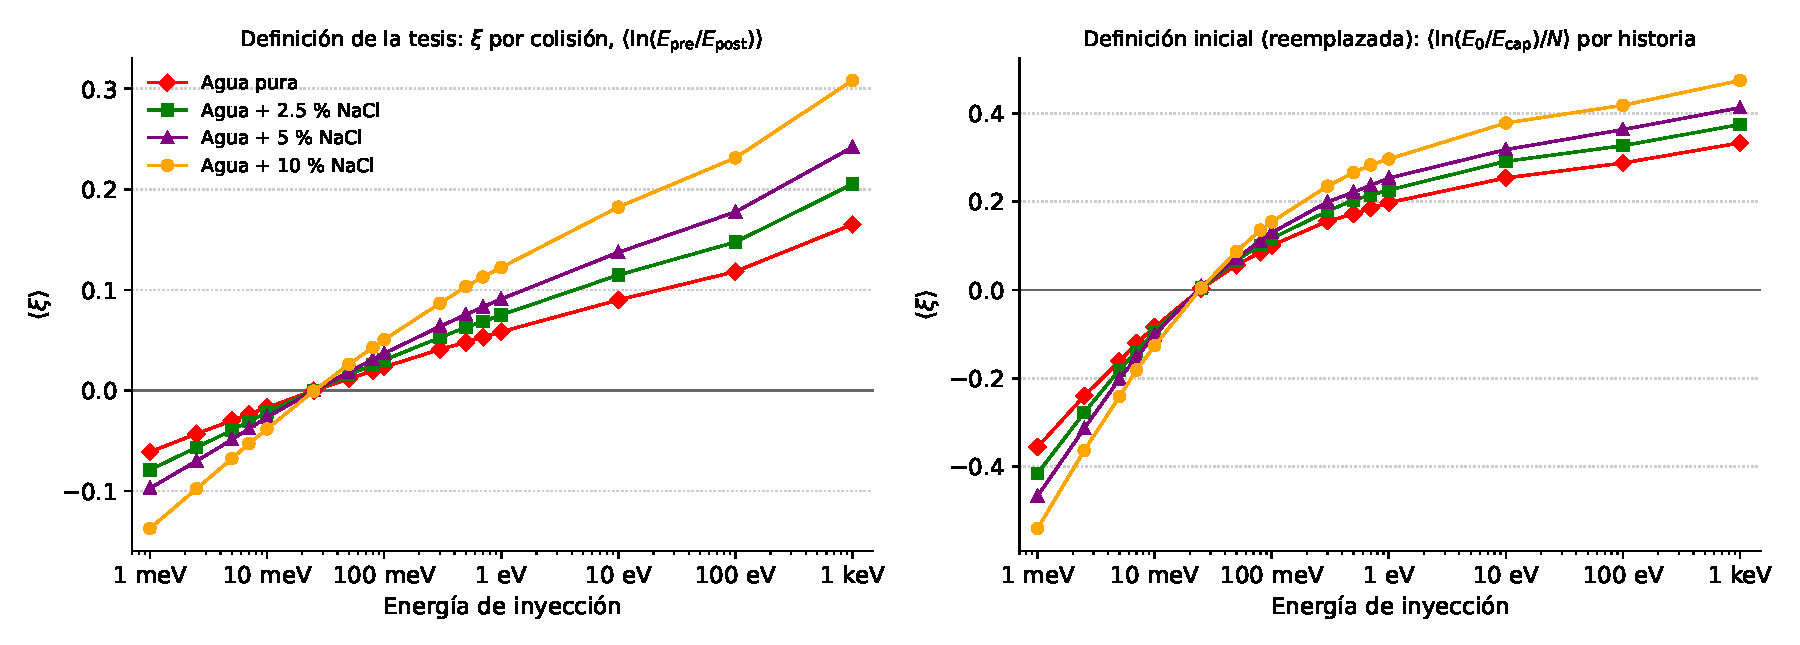
\includegraphics[width=\linewidth]{xi_medio.pdf}
  \caption{Izquierda: $\langle\xi\rangle$ por colisión (definición de la tesis) en función de la energía. Derecha, solo como referencia: la definición inicial por historia, reemplazada en el estudio. Ambas cambian de signo cerca de 25~meV, la energía térmica del medio a 20~$^\circ$C.}
  \label{fig:xi-medio}
\end{figure}

La Figura~\ref{fig:xi-medio} resume las cuatro regiones: $\langle\xi\rangle<0$ por debajo de la energía térmica, $\langle\xi\rangle\simeq0$ alrededor de 25~meV y $\langle\xi\rangle>0$ y creciente por encima; el valor absoluto es mayor con NaCl, de forma coherente con historias capturadas más cortas. En conjunto, el hidrógeno conserva el papel principal como moderador. La estabilidad de la forma y de $\sigma(\xi)$ muestra que las historias capturadas comparten un patrón estadístico semejante, pero no prueba que la moderación global sea idéntica; el efecto demostrado del dopante es el cambio de la probabilidad de captura, y su efecto específico sobre la moderación exige un análisis por núcleo dispersor.

% =====================================================================
\section{Balance de captura, reflexión y transmisión}
\label{sec:balance}

\subsection{Eficiencia de captura}

$\eta_\mathrm{Cap}$ es la fracción de neutrones primarios absorbidos. Es una etapa necesaria de la respuesta del WCD, pero no su eficiencia final de detección: después de la captura, la radiación gamma y las partículas cargadas secundarias deben producir luz Cherenkov que alcance el fotomultiplicador (Sección~\ref{sec:enlace}). Más del 98~\% de las capturas ocurre dentro del volumen activo; el resto, en la tapa o en el aire.

\begin{figure}[H]
  \centering
  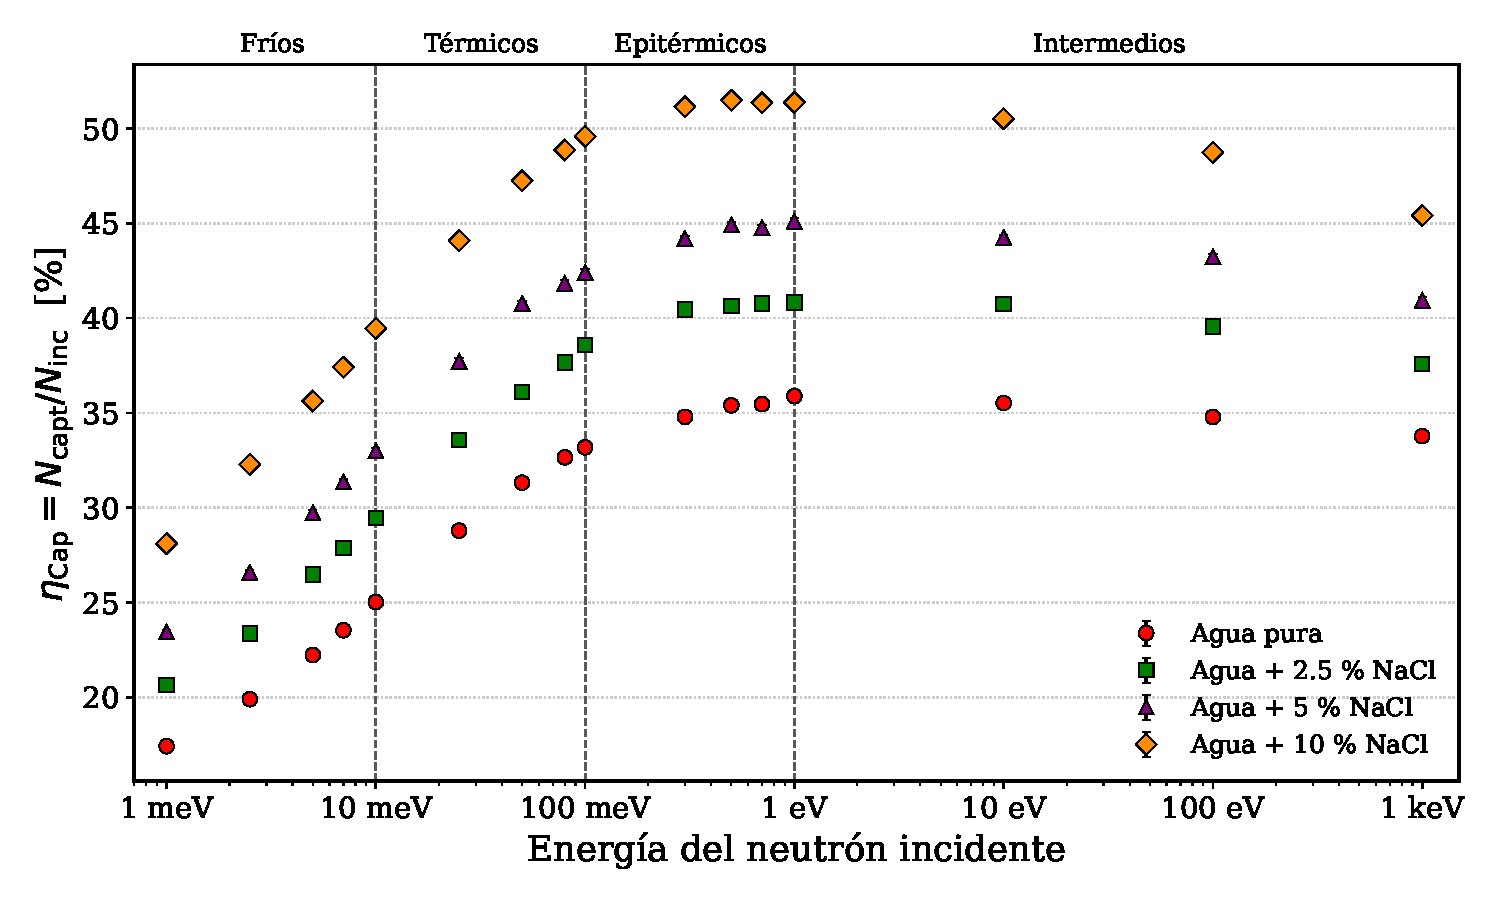
\includegraphics[width=0.92\linewidth]{fig_4_24_captura.pdf}
  \caption{Eficiencia de captura $\eta_\mathrm{Cap}$ en función de la energía para los cuatro medios (Figura~4.24 de la tesis). Barras de error: incertidumbre estándar marginal ($1\sigma$), menores que los símbolos.}
  \label{fig:captura}
\end{figure}

Los cuatro medios tienen la misma dependencia con la energía (Figura~\ref{fig:captura}): $\eta_\mathrm{Cap}$ aumenta desde 1~meV hasta una región de variación reducida entre unos 300~meV y 10~eV y disminuye suavemente hacia 1~keV. En agua pura pasa de $(17.418\pm0.120)$~\% a 1~meV a un máximo de $(35.881\pm0.152)$~\% a 1~eV y baja a $(33.772\pm0.150)$~\% a 1~keV. La forma resulta de la competencia entre moderación, captura y escape: un neutrón más energético necesita una historia de moderación más larga antes de llegar a energías donde la absorción es probable, y mientras tanto puede abandonar el volumen activo por la tapa.

El NaCl aumenta la captura en todas las energías. A 1~meV pasa de $(17.418\pm0.120)$~\% en agua pura a $(28.107\pm0.142)$~\% con 10~\% de NaCl, y a 1~eV, de $(35.881\pm0.152)$~\% a $(51.378\pm0.158)$~\%. Para una misma energía se cumple
\begin{equation}
\eta_\mathrm{Cap}^\mathrm{agua}<\eta_\mathrm{Cap}^{\text{2.5\,\%}}<\eta_\mathrm{Cap}^{\text{5\,\%}}<\eta_\mathrm{Cap}^{\text{10\,\%}},
\end{equation}
con diferencias mucho mayores que las incertidumbres estadísticas. El responsable es el $^{35}$Cl, cuya sección eficaz de absorción, $(43.84\pm0.17)$~b, es unas 132 veces la del $^1$H, $(0.3326\pm0.0007)$~b~\cite{Sidelnik2020}. Sidelnik et al.\ encontraron también que la captura crece con la concentración de NaCl sin alterar de forma apreciable la moderación~\cite{Sidelnik2020}, aunque para neutrones de 500~MeV con incidencia horizontal; la dependencia con la energía entre 1~meV y 1~keV de la Figura~\ref{fig:captura} es un resultado propio de estas simulaciones.

\begin{table}[H]
\centering
\small
\caption{Coeficientes de captura, reflexión, transmisión y otros destinos en agua pura, en porcentaje, con su incertidumbre estándar marginal (Tabla~4.8 de la tesis). La suma es 1 en todas las energías. Los demás medios están en el Apéndice~\ref{ap:tablas}.}
\label{tab:coef-AP}
\begin{tabular}{@{}lrrrr@{}}
\toprule
$E$ & $\eta_\mathrm{Cap}$ [\%] & $\eta_\mathrm{Refle}$ [\%] & $\eta_\mathrm{Trans}$ [\%] & $\eta_\mathrm{Otros}$ [\%] \\
\midrule
1 meV & $17.418\pm0.120$ & $76.569\pm0.134$ & $0.045\pm0.007$ & $5.968\pm0.075$ \\
2.5 meV & $19.899\pm0.126$ & $75.842\pm0.135$ & $0.043\pm0.007$ & $4.216\pm0.064$ \\
5 meV & $22.229\pm0.131$ & $74.291\pm0.138$ & $0.038\pm0.006$ & $3.442\pm0.058$ \\
7 meV & $23.532\pm0.134$ & $73.267\pm0.140$ & $0.042\pm0.006$ & $3.159\pm0.055$ \\
10 meV & $25.021\pm0.137$ & $72.086\pm0.142$ & $0.041\pm0.006$ & $2.852\pm0.053$ \\
25 meV & $28.790\pm0.143$ & $68.782\pm0.147$ & $0.043\pm0.007$ & $2.385\pm0.048$ \\
50 meV & $31.320\pm0.147$ & $66.328\pm0.149$ & $0.033\pm0.006$ & $2.319\pm0.048$ \\
80 meV & $32.654\pm0.148$ & $65.130\pm0.151$ & $0.042\pm0.006$ & $2.174\pm0.046$ \\
100 meV & $33.180\pm0.149$ & $64.589\pm0.151$ & $0.027\pm0.005$ & $2.204\pm0.046$ \\
300 meV & $34.790\pm0.151$ & $63.195\pm0.153$ & $0.041\pm0.006$ & $1.974\pm0.044$ \\
500 meV & $35.397\pm0.151$ & $62.595\pm0.153$ & $0.039\pm0.006$ & $1.969\pm0.044$ \\
700 meV & $35.463\pm0.151$ & $62.430\pm0.153$ & $0.052\pm0.007$ & $2.055\pm0.045$ \\
1 eV & $35.881\pm0.152$ & $62.168\pm0.153$ & $0.038\pm0.006$ & $1.913\pm0.043$ \\
10 eV & $35.522\pm0.151$ & $62.607\pm0.153$ & $0.049\pm0.007$ & $1.822\pm0.042$ \\
100 eV & $34.784\pm0.151$ & $63.362\pm0.152$ & $0.045\pm0.007$ & $1.809\pm0.042$ \\
1 keV & $33.772\pm0.150$ & $64.560\pm0.151$ & $0.042\pm0.006$ & $1.626\pm0.040$ \\
\bottomrule
\end{tabular}
\end{table}

\subsection{Reflexión}

La reflexión cuenta los neutrones que entran al medio, se dispersan y salen por la frontera de incidencia; cuantifica un destino final, no una ausencia de interacción. Es el destino dominante en agua pura y tiene la tendencia opuesta a la captura (Figura~\ref{fig:reflexion}): disminuye de $(76.569\pm0.134)$~\% a 1~meV a $(62.168\pm0.153)$~\% a 1~eV y vuelve a subir hasta $(64.560\pm0.151)$~\% a 1~keV. El mínimo amplio entre 300~meV y 10~eV coincide con el máximo de la captura.

\begin{figure}[H]
  \centering
  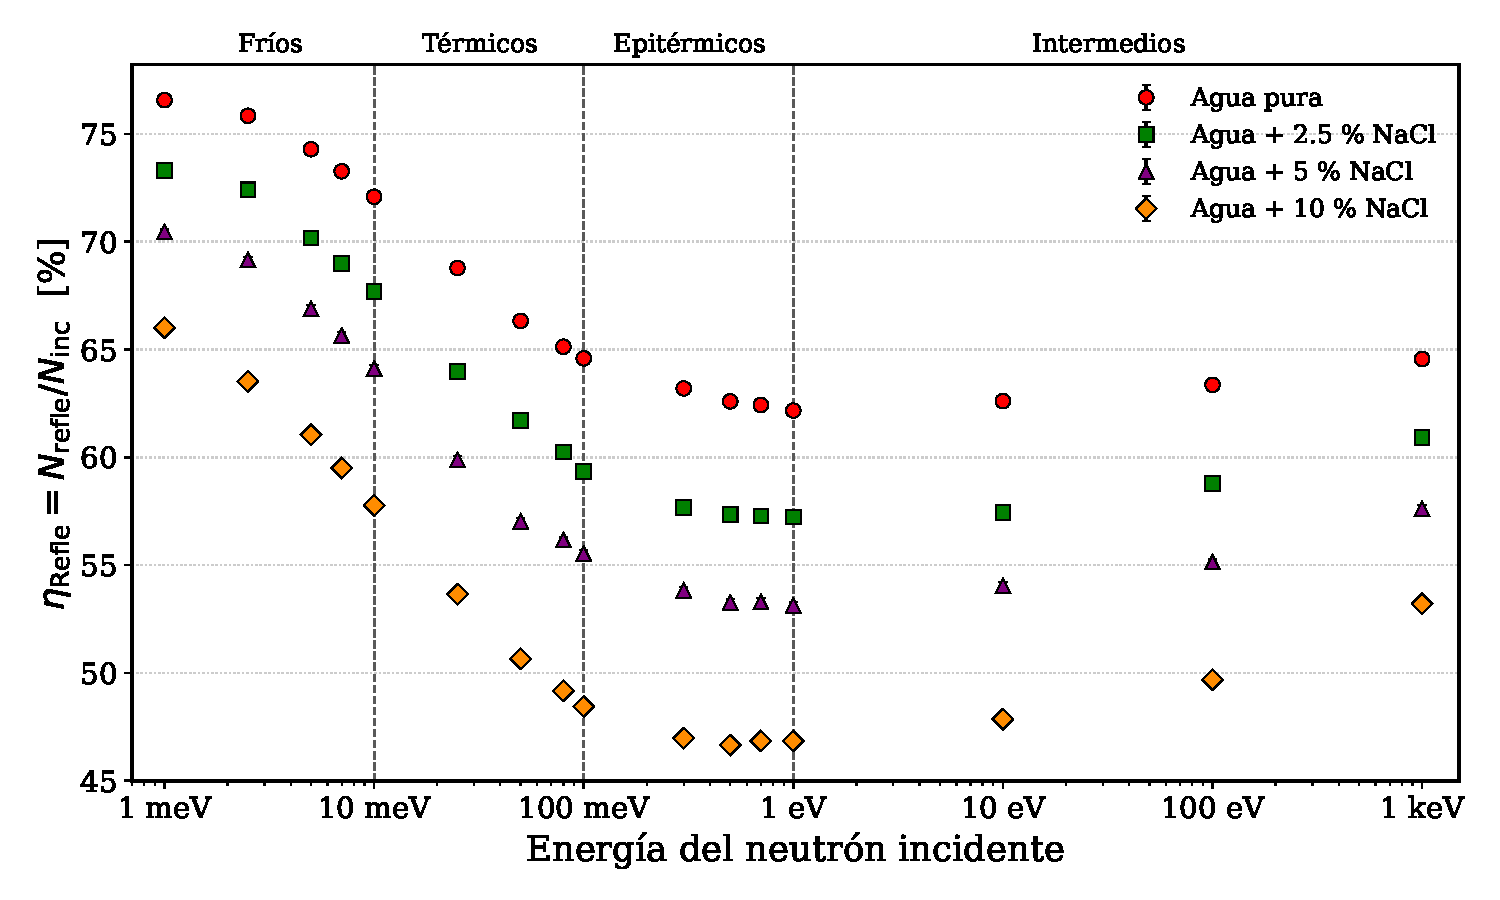
\includegraphics[width=0.92\linewidth]{fig_4_25_reflexion.pdf}
  \caption{Coeficiente de reflexión $\eta_\mathrm{Refle}$ (salida por la cara superior del volumen activo) en función de la energía (Figura~4.25 de la tesis).}
  \label{fig:reflexion}
\end{figure}

El NaCl reduce la reflexión de forma sistemática: a 1~meV, de 76.57 a 66.01~\% con 10~\% de NaCl, y a 1~eV, de 62.17 a 46.84~\%. La diferencia entre 5 y 10~\% no es despreciable (unos 6 puntos porcentuales cerca de 1~eV), de modo que estas curvas no muestran saturación ni permiten fijar una concentración óptima.

\subsection{Transmisión y otros destinos}

\begin{figure}[H]
  \centering
  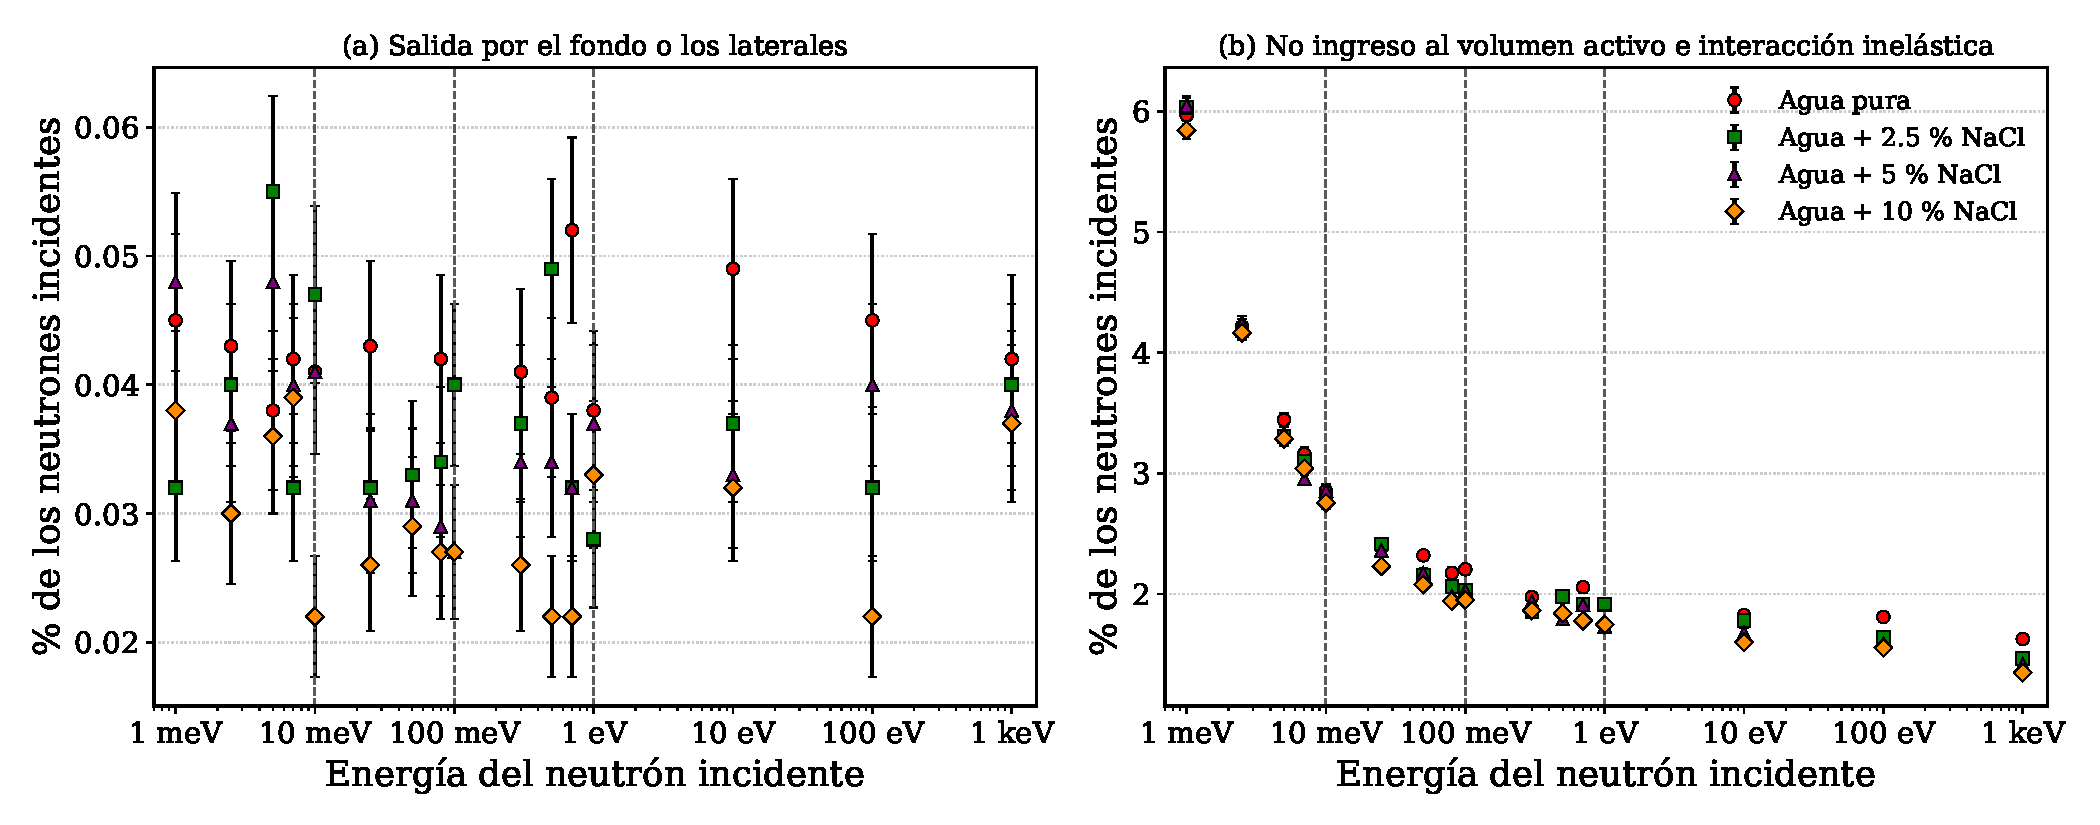
\includegraphics[width=\linewidth]{fig_4_26_transmision_otros.pdf}
  \caption{(a) Coeficiente de transmisión $\eta_\mathrm{Trans}$ (salida por el fondo o las paredes laterales) y (b) coeficiente de otros destinos $\eta_\mathrm{Otros}$ (neutrones que no entran al volumen activo o terminan en una interacción inelástica) (Figura~4.26 de la tesis).}
  \label{fig:trans-otros}
\end{figure}

La transmisión es prácticamente despreciable: entre 0.02 y 0.06~\% en todas las corridas, con incertidumbres de unos 0.006 puntos, sin dependencia sistemática con la energía ni con el medio. Los neutrones que entran por la tapa se moderan y capturan en los primeros centímetros (Sección~\ref{sec:lambda}), muy lejos del fondo y de las paredes. $\eta_\mathrm{Otros}$ disminuye en agua pura de $(5.968\pm0.075)$~\% a 1~meV a $(1.913\pm0.043)$~\% a 1~eV y $(1.626\pm0.040)$~\% a 1~keV; a 1~meV, 3.6 puntos corresponden a neutrones que no entran al volumen activo y 2.4 a interacciones inelásticas, en su mayoría fuera del medio. Este coeficiente casi no depende de la concentración, como corresponde a procesos que ocurren antes de que el neutrón alcance el agua.

\subsection{Discusión conjunta}

El NaCl no añade un destino nuevo: redistribuye las historias. Como la transmisión es despreciable y $\eta_\mathrm{Otros}$ casi no cambia con la concentración, el aumento de la captura se produce a expensas de la reflexión:
\begin{equation}
\Delta\eta_\mathrm{Cap}+\Delta\eta_\mathrm{Refle}+\Delta\eta_\mathrm{Trans}+\Delta\eta_\mathrm{Otros}=0,\qquad
\Delta\eta_\mathrm{Cap}\simeq-\Delta\eta_\mathrm{Refle}.
\end{equation}

En agua pura y con 2.5 y 5~\% de NaCl, la reflexión supera a la captura en todo el intervalo. Con 10~\%, ambas se igualan cerca de 80~meV (48.86 frente a 49.16~\%), la captura supera a la reflexión entre 100~meV y 10~eV, y a energías mayores la reflexión vuelve a dominar. Las incertidumbres marginales están entre 0.005 y 0.158 puntos porcentuales, muy por debajo de las diferencias entre medios, pero están correlacionadas por la Ecuación~\eqref{eq:balance} y no deben sumarse como independientes.

El balance completa la imagen de la Sección~\ref{sec:moderacion}: la disminución de \var{hadElastic} con el NaCl no indica pérdida de capacidad moderadora, sino que la mayor captura acorta una parte de las historias, reduce las dispersiones acumuladas y disminuye el escape por la tapa. Esa redistribución aumenta la producción potencial de radiación gamma de captura, punto de partida de la señal. La solución con 10~\% de NaCl tiene la mayor captura y la menor reflexión en todo el intervalo, pero estos resultados no bastan para elegir una concentración óptima: hacen falta también la respuesta óptica, el número de fotoelectrones, la eficiencia final, la estabilidad de la solución y las incertidumbres sistemáticas del modelo.

\subsection{Ganancia relativa de captura}

\begin{figure}[H]
  \centering
  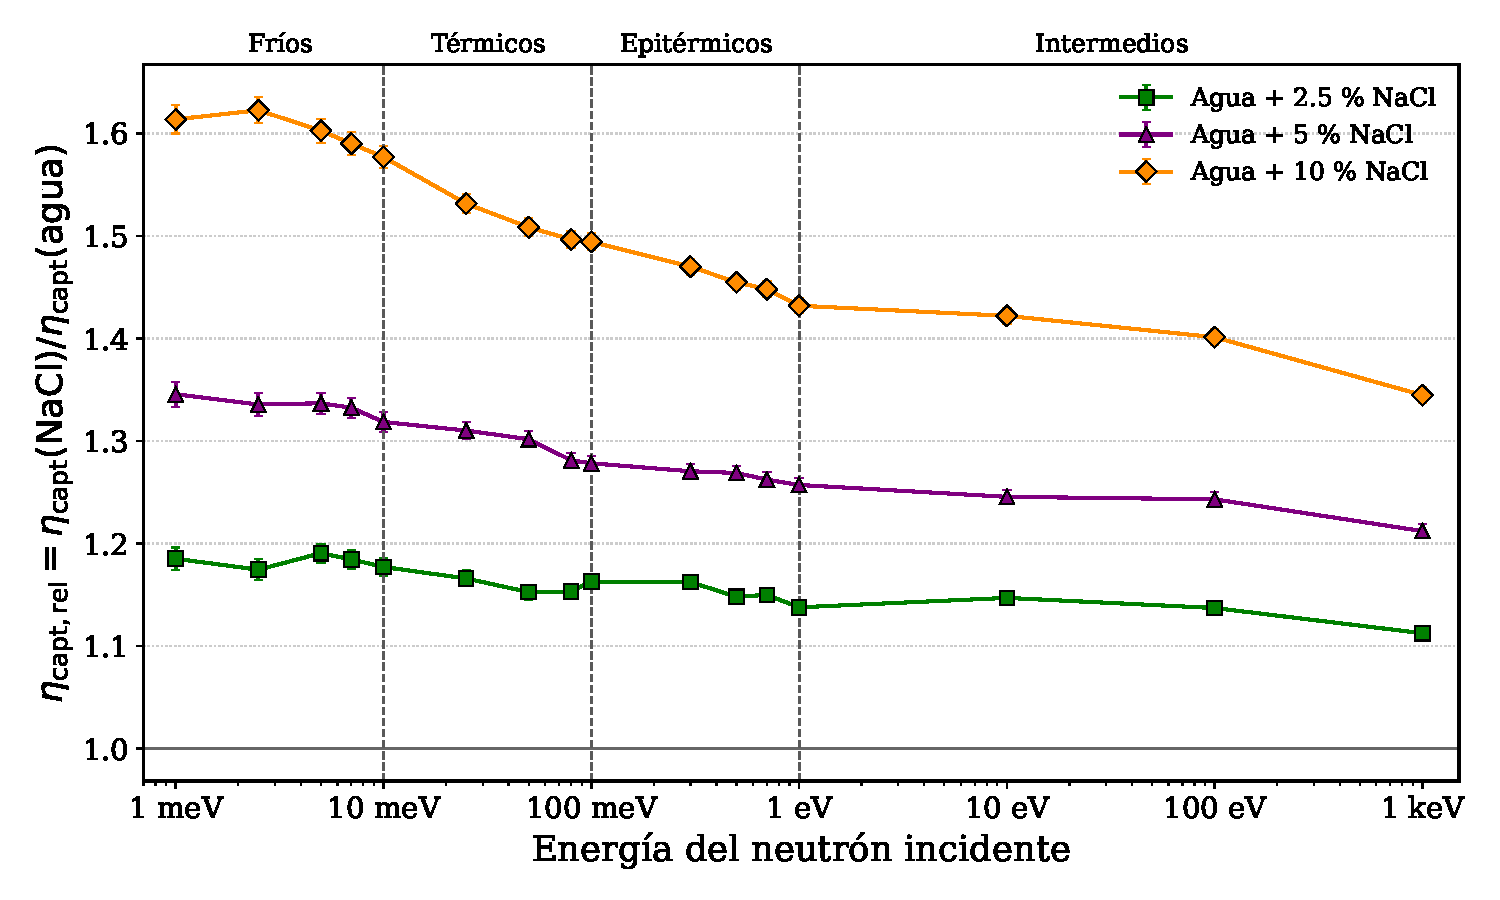
\includegraphics[width=0.92\linewidth]{fig_4_27_captura_relativa.pdf}
  \caption{Ganancia relativa de captura $\eta_\mathrm{Cap}(\mathrm{NaCl})/\eta_\mathrm{Cap}(\mathrm{agua})$ (Figura~4.27 de la tesis).}
  \label{fig:cap-rel}
\end{figure}

Las tres curvas están por encima de la unidad en todo el intervalo (Figura~\ref{fig:cap-rel}). La ganancia es mayor a baja energía (1.19, 1.35 y 1.61 a 1~meV con 2.5, 5 y 10~\%) y disminuye hacia 1~keV (1.11, 1.21 y 1.34). Esta tendencia es compatible con la gran absorción térmica del $^{35}$Cl y con la competencia entre captura y escape, pero la razón macroscópica no es una medida directa de una ley $1/v$: contiene también moderación, composición, geometría y selección de historias. La separación persistente entre 5 y 10~\% indica que la captura no está saturada por encima de 5~\%.

% =====================================================================
\section{Distribución espacial y longitud de captura}
\label{sec:lambda}

\subsection{Profundidad de captura}

\begin{figure}[H]
  \centering
  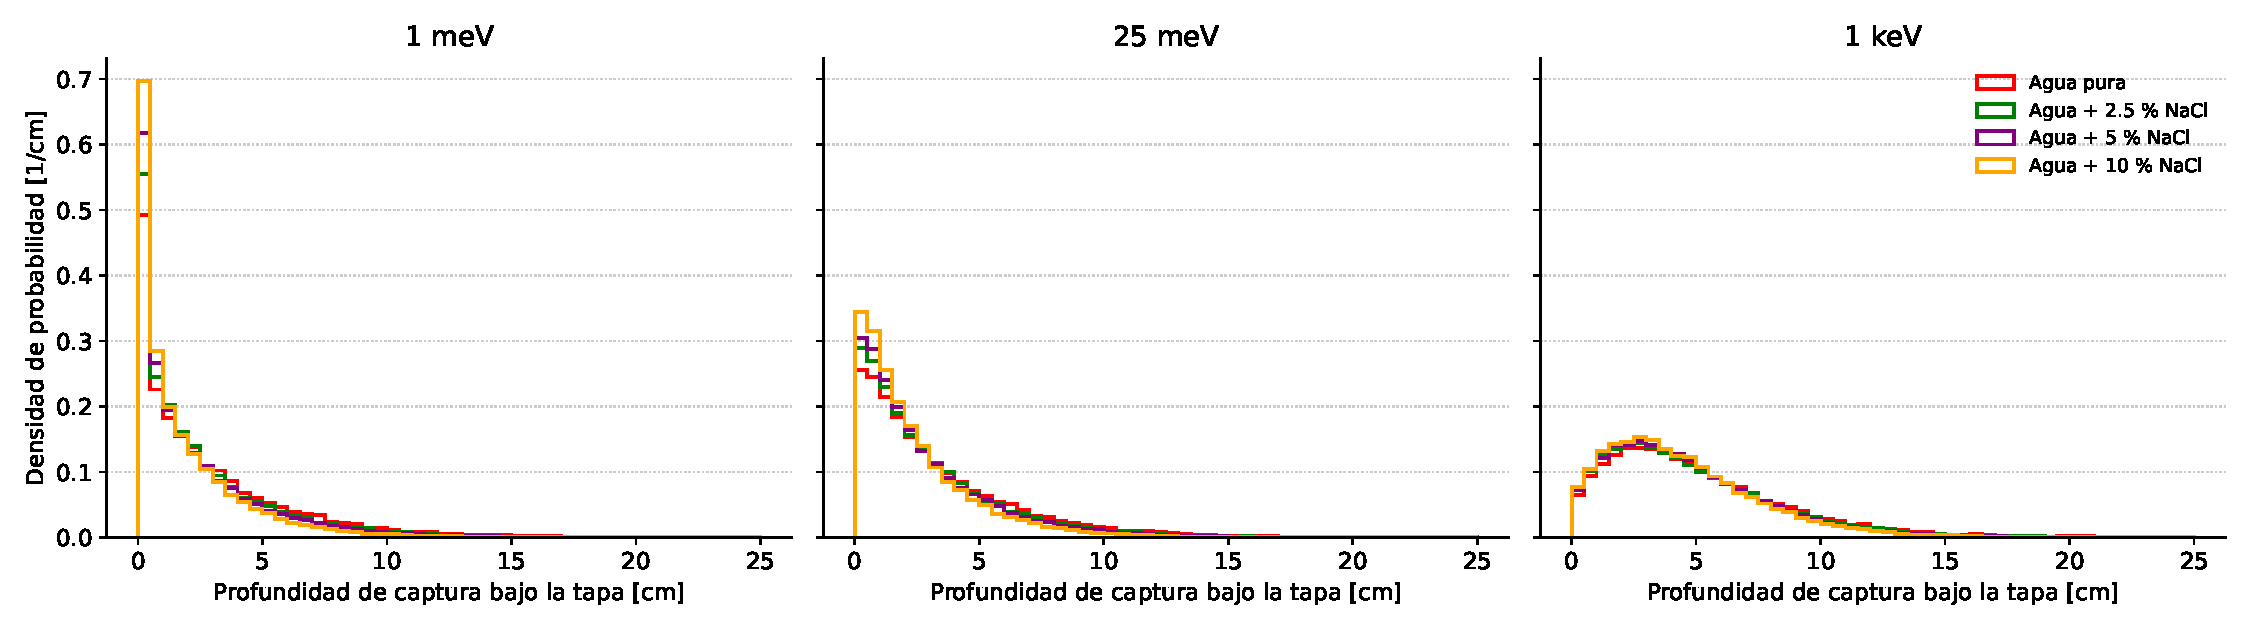
\includegraphics[width=\linewidth]{profundidad_captura.pdf}
  \caption{Profundidad de captura bajo la cara interior de la tapa ($z=1330$~mm) para las capturas dentro del volumen activo.}
  \label{fig:prof}
\end{figure}

Las capturas se concentran en los primeros centímetros bajo la tapa (Figura~\ref{fig:prof}). En agua pura, la profundidad mediana pasa de 1.8~cm a 1~meV a 4.3~cm a 1~keV, y el 90~\% de las capturas ocurre a menos de 7--10~cm; con 10~\% de NaCl, las capturas son más superficiales (mediana de 1.0~cm a 1~meV). Por eso la transmisión por el fondo y las paredes es despreciable.

\subsection{Longitud de captura}

\begin{figure}[H]
  \centering
  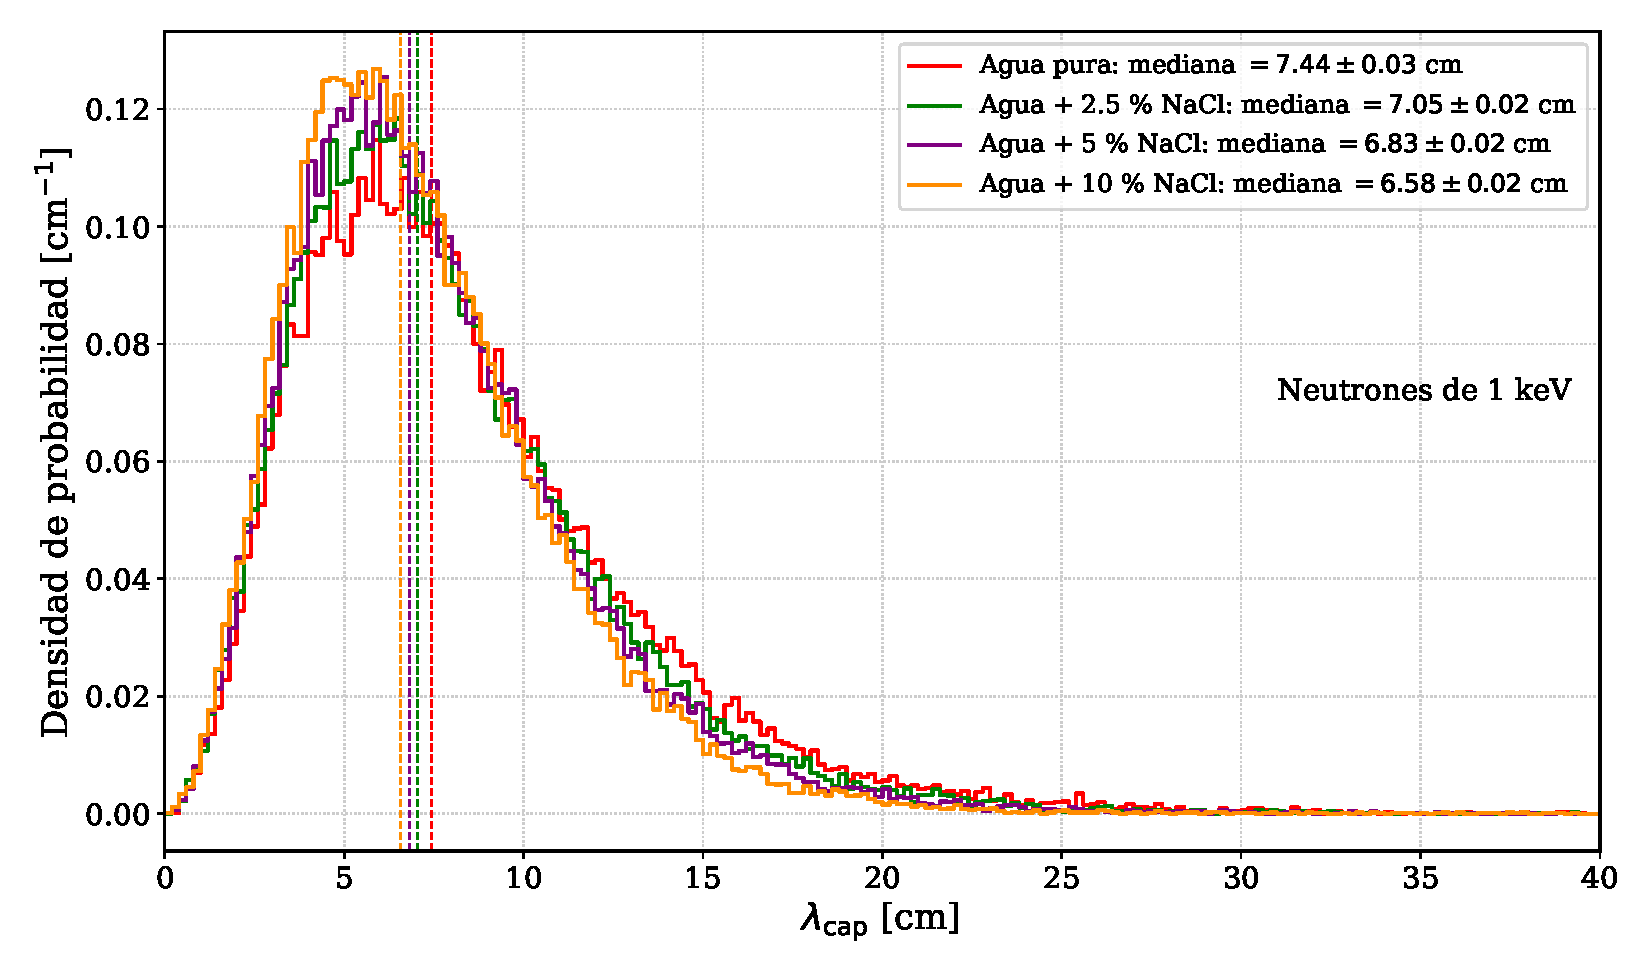
\includegraphics[width=0.92\linewidth]{fig_4_28_lambda_cap_1keV.pdf}
  \caption{Distribución de $\lambda_\mathrm{cap}$ para neutrones de 1~keV en los cuatro medios, normalizada a área unitaria con intervalos de 0.2~cm; las líneas discontinuas marcan la mediana (Figura~4.28 de la tesis).}
  \label{fig:lambda-1keV}
\end{figure}

La distribución de $\lambda_\mathrm{cap}$ es asimétrica, con una cola larga hacia distancias mayores (Figura~\ref{fig:lambda-1keV}). A 1~keV, la mediana es $(7.44\pm0.03)$~cm en agua pura (percentiles 25--75: 5.04--10.64~cm), $(7.05\pm0.02)$, $(6.83\pm0.02)$ y $(6.58\pm0.02)$~cm con 2.5, 5 y 10~\% de NaCl (10~\%: 4.56--9.16~cm).

\begin{table}[H]
\centering
\small
\caption{Mediana de la longitud de captura $\lambda_\mathrm{cap}$ [cm] por energía y medio, con su incertidumbre estadística por remuestreo (Tabla~4.9 de la tesis).}
\label{tab:lambda}
\begin{tabular}{@{}lcccc@{}}
\toprule
$E$ & Agua pura & Agua + 2.5~\% & Agua + 5~\% & Agua + 10~\% \\
\midrule
\csname @@input\endcsname \tablaanalisis/tabla_4_9_lambda_cap.tex
\bottomrule
\end{tabular}
\end{table}

\begin{figure}[H]
  \centering
  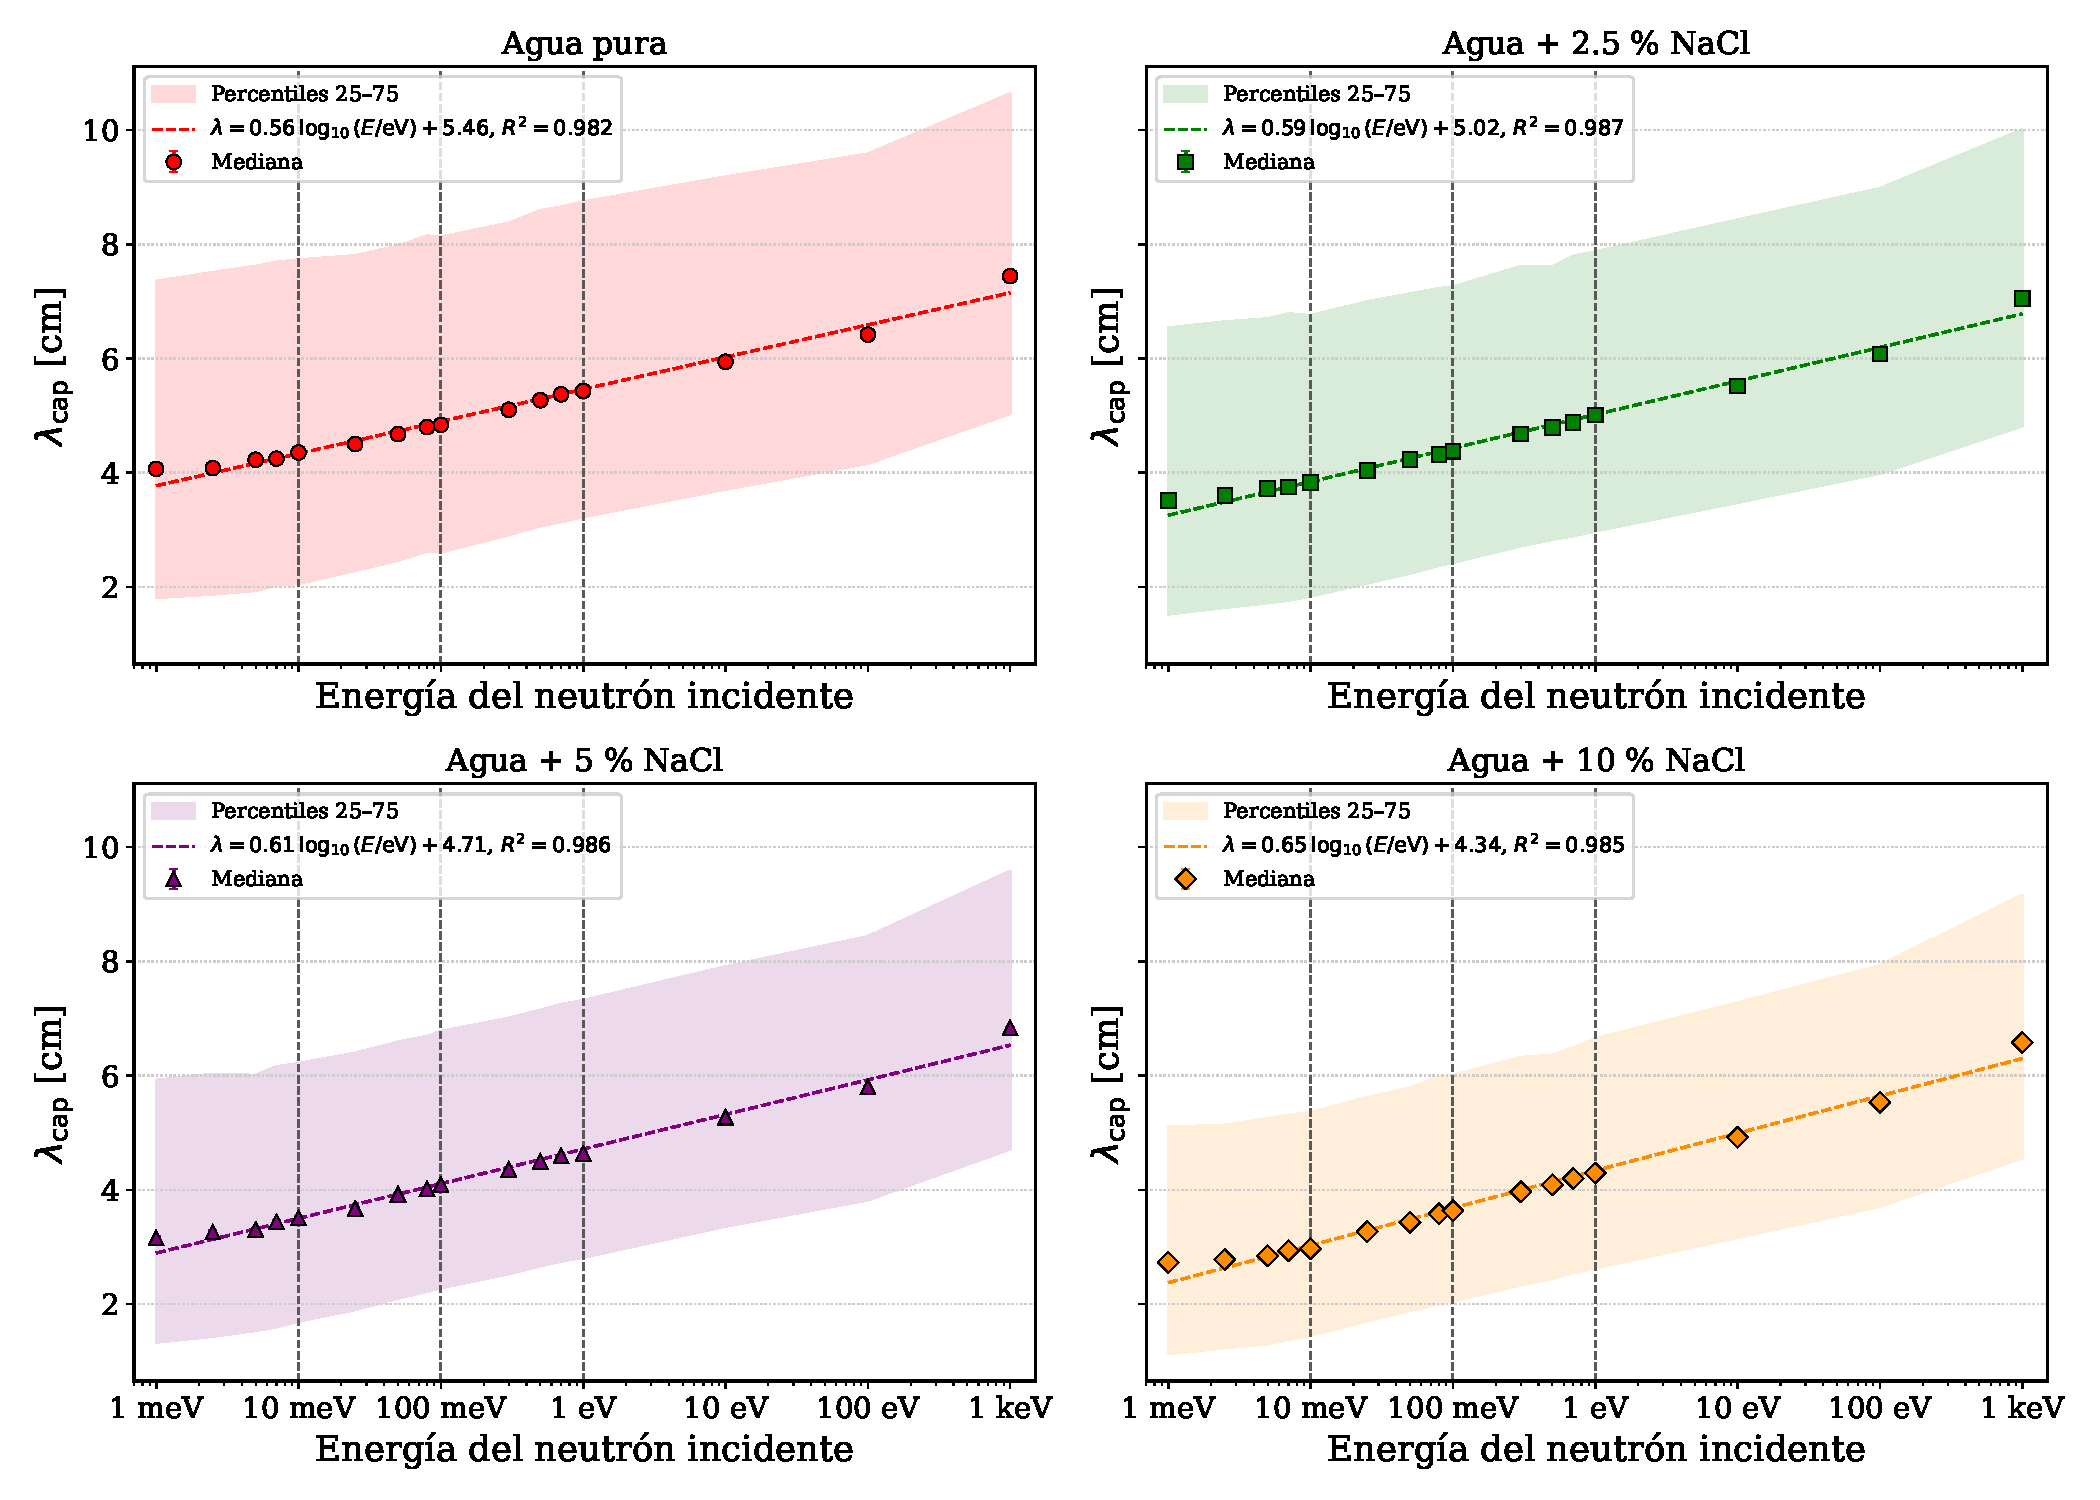
\includegraphics[width=0.92\linewidth]{fig_4_29_lambda_cap_vs_energia.pdf}
  \caption{Mediana de $\lambda_\mathrm{cap}$ (símbolos), intervalo entre los percentiles 25 y 75 (banda) y ajuste lineal en $\log_{10}(E/\mathrm{eV})$ (línea discontinua) (Figura~4.29 de la tesis).}
  \label{fig:lambda-E}
\end{figure}

La mediana aumenta de forma monótona con la energía en los cuatro medios (Tabla~\ref{tab:lambda} y Figura~\ref{fig:lambda-E}): en agua pura, de 4.07~cm a 1~meV a 7.44~cm a 1~keV, y con 10~\% de NaCl, de 2.73 a 6.58~cm. La dependencia es aproximadamente lineal en el logaritmo de la energía ($R^2\ge0.98$): el ajuste da 5.46, 5.02, 4.71 y 4.34~cm a 1~eV y pendientes de 0.56, 0.59, 0.61 y 0.65~cm por década para agua pura y 2.5, 5 y 10~\% de NaCl, de modo que las curvas se acercan a altas energías.

El NaCl reduce la longitud de captura en todas las energías, en concordancia con el aumento de la sección eficaz macroscópica de absorción, y la reducción es mayor a baja energía: entre agua pura y 10~\% de NaCl, 33~\% a 1~meV, 21~\% a 1~eV y 12~\% a 1~keV. Un neutrón frío o térmico se captura durante la difusión térmica cerca de la tapa, y el cloro acorta esa difusión; en un neutrón más energético, una parte creciente del recorrido corresponde al frenado previo, sobre el que el NaCl influye poco. Las diferencias entre medios son muy superiores a las incertidumbres de las medianas (0.01--0.04~cm), aunque las distribuciones se superponen ampliamente.

% =====================================================================
\section{Enlace con la respuesta electromagnética}
\label{sec:enlace}

El WCD no detecta el neutrón directamente, porque es eléctricamente neutro. La señal resulta de la cadena
\[
\mathrm{n}\;\longrightarrow\;\text{moderación y captura}\;\longrightarrow\;\gamma_\mathrm{Cap}\;\longrightarrow\;e^-,\,e^+\;\longrightarrow\;\text{radiación Cherenkov}\;\longrightarrow\;\mathrm{PMT}.
\]
Este informe cubre el primer eslabón, que es el único en el que interviene el neutrón. A partir de la captura, la señal depende de la cascada gamma del núcleo que captura (con energías de unos 0.47 a 8.6~MeV), de la interacción de esos fotones con el medio (Compton y producción de pares), de los electrones y positrones secundarios, de la producción de luz Cherenkov y de su transporte hasta el fotomultiplicador~\cite{Knoll2010}.

La eficiencia de detección del WCD, $\varepsilon(E_n,C)$, la fracción de neutrones incidentes que producen al menos un fotoelectrón, se factoriza de manera natural como
\begin{equation}
\varepsilon(E_n,C)=\eta_\mathrm{Cap}(E_n,C)\times P(\text{señal}\mid\text{captura};E_n,C).
\end{equation}
El primer factor es el resultado central de este informe y es una cota superior de la eficiencia. El segundo es de naturaleza electromagnética y óptica: depende sobre todo del núcleo que captura y, por tanto, de la concentración de NaCl. La carga por evento (Figuras~4.48 y 4.50 de la tesis), el número de fotones Cherenkov (Figura~4.49), la eficiencia de detección (Figura~4.51), su interpretación como función de respuesta con incidencia normal y la comparación cualitativa con los detectores CRS1000~\cite{Kohli2018} se presentan en el informe técnico de la respuesta electromagnética. Los datos de carga ya están procesados en los mismos \archivo{resumen.json} y en \archivo{resumen_campana.tsv}, de modo que ese informe no necesita reprocesar las corridas.

% =====================================================================
\section{Observaciones sobre el análisis original}
\label{sec:observaciones}

\begin{itemize}
  \item \textbf{Caja de selección.} El notebook original selecciona los pasos con una caja cuadrada de $\pm478$~mm en $x$ e $y$, mientras que el volumen activo es un cilindro de 480~mm de radio, y en otra celda usa límites de $\pm480$~mm y 1300~mm. Este procesamiento conserva la caja de $\pm478$~mm para $N$ (el $\xi$ de la tesis no depende de esta selección), porque es la que produjo las cifras de la tesis, y usa el volumen activo de los demás scripts para el destino final. La Sección~\ref{sec:cilindro} cuantifica el efecto de reemplazar la caja por el cilindro.
  %\item \textbf{Archivos duplicados o mal rotulados.} En la carpeta de 1~meV en agua pura, \archivo{Energia-transferida-nucleos-CITA-AP-Bga.txt} es idéntico al archivo de 1~meV pese a su nombre, y \archivo{numero-dispersiones-elasticas-AP-1meV-Bga.txt} está vacío. Este procesamiento no los usa.
  \item \textbf{Origen de los conteos por proceso.} Los archivos \archivo{hadElastic-*.txt} y equivalentes no los genera el notebook de la carpeta; se reproducen exactamente desde los datos crudos.
  \item \textbf{Tabla~4.9 anterior.} La versión anterior de la tesis daba, para once energías, la posición y el ancho de ajustes gaussianos al pico de la distribución de $\lambda_\mathrm{cap}$, con intervalos de ajuste introducidos a mano en cada notebook. El script \archivo{verificar_tabla_4_9_original.py} repite esos ajustes con los intervalos registrados.
  % y reproduce 33 de los 44 valores. Además, mostró que el archivo de 100~eV en agua pura era una copia del de 1~keV, que los de 700~meV con 2.5 y 5~\% de NaCl no provienen de los datos de la Campaña~1 y que el ``$\pm$'' de la tabla era el ancho de la gaussiana, no una incertidumbre. Como el máximo es ancho y la distribución asimétrica, la moda es inestable (a 1~keV en agua pura, el ajuste anterior daba 6.43~cm, la moda 5.8--6.0~cm según el intervalo, la mediana 7.44~cm y la media 8.48~cm); por eso la versión final usa la mediana (Sección~\ref{sec:lambda-metodo}).
  \item \textbf{Archivos intermedios.} El notebook generaba archivos de hasta 185~MB por corrida; el procesamiento nuevo no necesita ninguno.
\end{itemize}

% =====================================================================
\section{Caja frente a cilindro}
\label{sec:cilindro}

Para cuantificar el efecto de seleccionar los pasos con una caja cuadrada, las 64 corridas se reprocesaron con un cilindro de radio $R = 480$~mm, el radio del tanque en la configuración del simulador (\var{tankRadius} = 48~cm). Un punto se considera dentro del tanque si
\[
r = \sqrt{x^2 + y^2} \le R ,
\]
con los mismos límites en $z$ que la caja. El cilindro sustituye tanto la caja de $\pm478$~mm usada para $N$ como la de $\pm480$~mm usada para el destino final. La comparación se hace neutrón por neutrón con el script \archivo{comparar_cilindro.py}.

\begin{center}
\small
\begin{tabular}{@{}llrrrrrrrr@{}}
\toprule
& & \multicolumn{2}{c}{$\eta_\mathrm{Refle}$ [\%]} & \multicolumn{2}{c}{$\eta_\mathrm{Trans}$ [\%]} & \multicolumn{2}{c}{$\langle N\rangle$} & \multicolumn{2}{c}{Neutrones que cambian} \\
\cmidrule(lr){3-4}\cmidrule(lr){5-6}\cmidrule(lr){7-8}\cmidrule(l){9-10}
Medio & $E$ & caja & cilindro & caja & cilindro & caja & cilindro & destino & $N$ \\
\midrule
\csname @@input\endcsname figuras-procesamiento-64-corridas/tabla_caja_cilindro.tex
\bottomrule
\end{tabular}
\end{center}

En el conjunto de las 64 corridas:

\begin{itemize}
  \item la captura, dentro y fuera del volumen activo, es idéntica con ambas geometrías;
  \item entre 16 y 61 de cada 100\,000 neutrones cambian de destino: se contaban como reflejados por la tapa y, con el cilindro, salen por la pared lateral. La reflexión disminuye y la transmisión aumenta como máximo en 0.031 puntos porcentuales, menos de una cuarta parte de la incertidumbre estadística de la reflexión (0.13--0.16 puntos); los otros destinos cambian como máximo en 0.002 puntos;
  \item el número de cadenas válidas para $N$ cambia como máximo en una, como máximo 8 de cada 100\,000 neutrones tienen un valor distinto de $N$, y $\langle N\rangle$ cambia menos del 0.005~\%; $\langle\xi\rangle$ cambia como máximo en $2\times10^{-5}$.
\end{itemize}

La diferencia es pequeña porque los neutrones se inyectan dentro de un disco de 25~cm de radio centrado en el eje del tanque, de modo que muy pocos alcanzan las esquinas de la caja ($r > 480$~mm), que ya están fuera del agua. La caja cuadrada del análisis original es, por tanto, una aproximación válida, y ninguna cifra de la tesis cambia al usar el cilindro.

% =====================================================================
\section{Reproducibilidad}
\label{sec:reproducibilidad}

El notebook \archivo{figuras_seccion_4.2.ipynb} (generado por \archivo{construir_notebook.py}) regenera, solo a partir de \archivo{resumen_campana.tsv} y de los \archivo{resumen.json}, las Figuras~4.17--4.29 y D.1--D.6 y la Tabla~4.9 de la tesis (y también las figuras de carga y eficiencia que usará el informe de la respuesta electromagnética), en PDF y PNG en \archivo{figuras-seccion-4.2/}. Este informe toma esas figuras directamente de esa carpeta. La última celda del notebook compara automáticamente 25 cifras con los valores de la tesis, entre ellas los $x_\mathrm{max}$ y FWHM de la Figura~4.19, y todas coinciden.

Desde la carpeta \archivo{analysis/campana-1_neutrones-monoenergeticos_seccion-4.2/} del repositorio:

\begin{lstlisting}
python3 procesar_campana.py <carpeta Neutrones-termicos> resultados 8
python3 comparar_cilindro.py <carpeta Neutrones-termicos> resultados resultados-cilindro 8
python3 construir_notebook.py
jupyter nbconvert --to notebook --execute figuras_seccion_4.2.ipynb
python3 figuras_informe.py resultados \
  ../../docs/technical-reports/campana-1_sin-S-alpha-beta/figuras-procesamiento-64-corridas
python3 tablas_seccion_4_2.py resultados \
  ../../docs/technical-reports/campana-1_sin-S-alpha-beta/figuras-procesamiento-64-corridas
\end{lstlisting}

El primer comando tarda alrededor de un minuto con ocho procesos y escribe 119~MB; el segundo, que solo se necesita para la Sección~\ref{sec:cilindro}, tarda otro minuto y escribe otros 119~MB; los demás, unos segundos. Solo se requieren Python~3, NumPy y Matplotlib (y Jupyter para el notebook).

Se publican en el repositorio los scripts, este informe, \archivo{resumen_campana.tsv}, los 64 \archivo{resumen.json} y \archivo{comparacion_caja_cilindro.tsv} (menos de 1~MB); las 64 tablas \archivo{historias.tsv.gz} se depositarán en Zenodo junto con los archivos crudos y sus sumas SHA-256.

% =====================================================================
\section{Conclusiones}

\begin{enumerate}
  \item Las 64 corridas de la Campaña~1 se procesan desde los archivos crudos con dos scripts, sin archivos intermedios y en alrededor de un minuto, y reproducen exactamente el balance de destinos, los conteos por proceso, las cadenas de dispersión, las distribuciones de $\xi$ y todas las cifras de la Campaña~1 que citan los Capítulos~4 y~5. Un notebook regenera todas las figuras de la parte neutrónica de la Sección~4.2.
  \item Los neutrones que entran por la tapa se moderan y capturan en los primeros centímetros del agua: la longitud de captura mediana va de 4.1 a 7.4~cm en agua pura entre 1~meV y 1~keV, y la transmisión por el fondo y las paredes es despreciable (0.02--0.06~\%). El balance se reparte casi por completo entre captura y reflexión por la tapa.
  \item El número de dispersiones elásticas antes de la captura crece con la energía ($\langle N\rangle$ de 44.8 a 76.8 en agua pura) y su distribución se desplaza y ensancha; las colas para $N\gtrsim100$ son comunes a todas las energías.
  \item La letargía por colisión refleja el equilibrio térmico del medio: $\langle\xi\rangle<0$ por debajo de unos 25~meV (el neutrón gana energía), $\langle\xi\rangle\simeq0$ en la energía térmica y $\langle\xi\rangle>0$ y creciente por encima, con $\sigma(\xi)\simeq1$ en todos los casos. El hidrógeno conserva el papel principal como moderador; los cambios de $\langle\xi\rangle$ con la salinidad son propiedades de la población de historias capturadas y no una mejora intrínseca de la moderación.
  \item La captura en agua pura sube de 17.4~\% a 1~meV a un máximo de 35.9~\% a 1~eV y baja a 33.8~\% a 1~keV. El NaCl la aumenta en todas las energías, hasta 51.4~\% con 10~\% de NaCl a 1~eV, casi enteramente a expensas de la reflexión. La ganancia relativa es mayor a baja energía (1.61 a 1~meV con 10~\%) y no muestra saturación entre 5 y 10~\%.
  \item El NaCl acorta la longitud de captura, con mayor efecto a baja energía (33~\% a 1~meV, 12~\% a 1~keV con 10~\%), porque actúa sobre la difusión térmica y poco sobre el frenado previo.
  \item La captura es la cota superior de la eficiencia de detección. El factor restante, la probabilidad de que una captura produzca señal, es electromagnético y óptico y se documenta, junto con la carga y la eficiencia del WCD, en el informe técnico de la respuesta electromagnética.
  \item Reemplazar la caja cuadrada por el cilindro de 480~mm cambia los coeficientes como máximo en 0.031 puntos porcentuales y $\langle N\rangle$ en menos del 0.005~\%; la aproximación del análisis original es válida.
\end{enumerate}

% =====================================================================
\appendix

\section{Tablas por medio}
\label{ap:tablas}

En todas las tablas, $\eta$ está en porcentaje, $\langle\xi\rangle$ es el $\xi$ de la tesis (por colisión), $\langle\xi\rangle_\mathrm{ini}$ el de la definición inicial (solo por trazabilidad) y $\bar{Q}$ la carga media en fotoelectrones por evento con señal, que se analiza en el informe de la respuesta electromagnética. Las incertidumbres de los coeficientes de agua pura están en la Tabla~\ref{tab:coef-AP}; para los demás medios son del mismo orden (Ecuación~\eqref{eq:incertidumbre}).

\newcommand{\tablamedio}[2]{%
\begin{center}
\small
\textbf{#2}\\[0.2em]
\begin{tabular}{@{}lrrrrrrrr@{}}
\toprule
$E$ & $\eta_\mathrm{Cap}$ & $\eta_\mathrm{Refle}$ & $\eta_\mathrm{Trans}$ & $\eta_\mathrm{Otros}$ & $\langle N\rangle$ & $\langle\xi\rangle$ & $\langle\xi\rangle_\mathrm{ini}$ & $\bar{Q}$ \\
\midrule
\csname @@input\endcsname figuras-procesamiento-64-corridas/tabla_#1.tex
\bottomrule
\end{tabular}
\end{center}}

\tablamedio{Agua-pura}{Agua pura}
\tablamedio{Agua+2.5NaCl}{Agua + 2.5~\% de NaCl}
\tablamedio{Agua+5NaCl}{Agua + 5~\% de NaCl}
\tablamedio{Agua+10NaCl}{Agua + 10~\% de NaCl}

\section{Distribuciones complementarias de $\xi$}
\label{ap:xi}

La tesis muestra las distribuciones de $\xi$ de los regímenes térmico, epitérmico e intermedio solo para agua pura. El notebook genera también las de los medios con NaCl, que se reúnen aquí; sus medias y desviaciones están en las Tablas~\ref{tab:xi-termica}--\ref{tab:xi-intermedia}.

\begin{figure}[H]
  \centering
  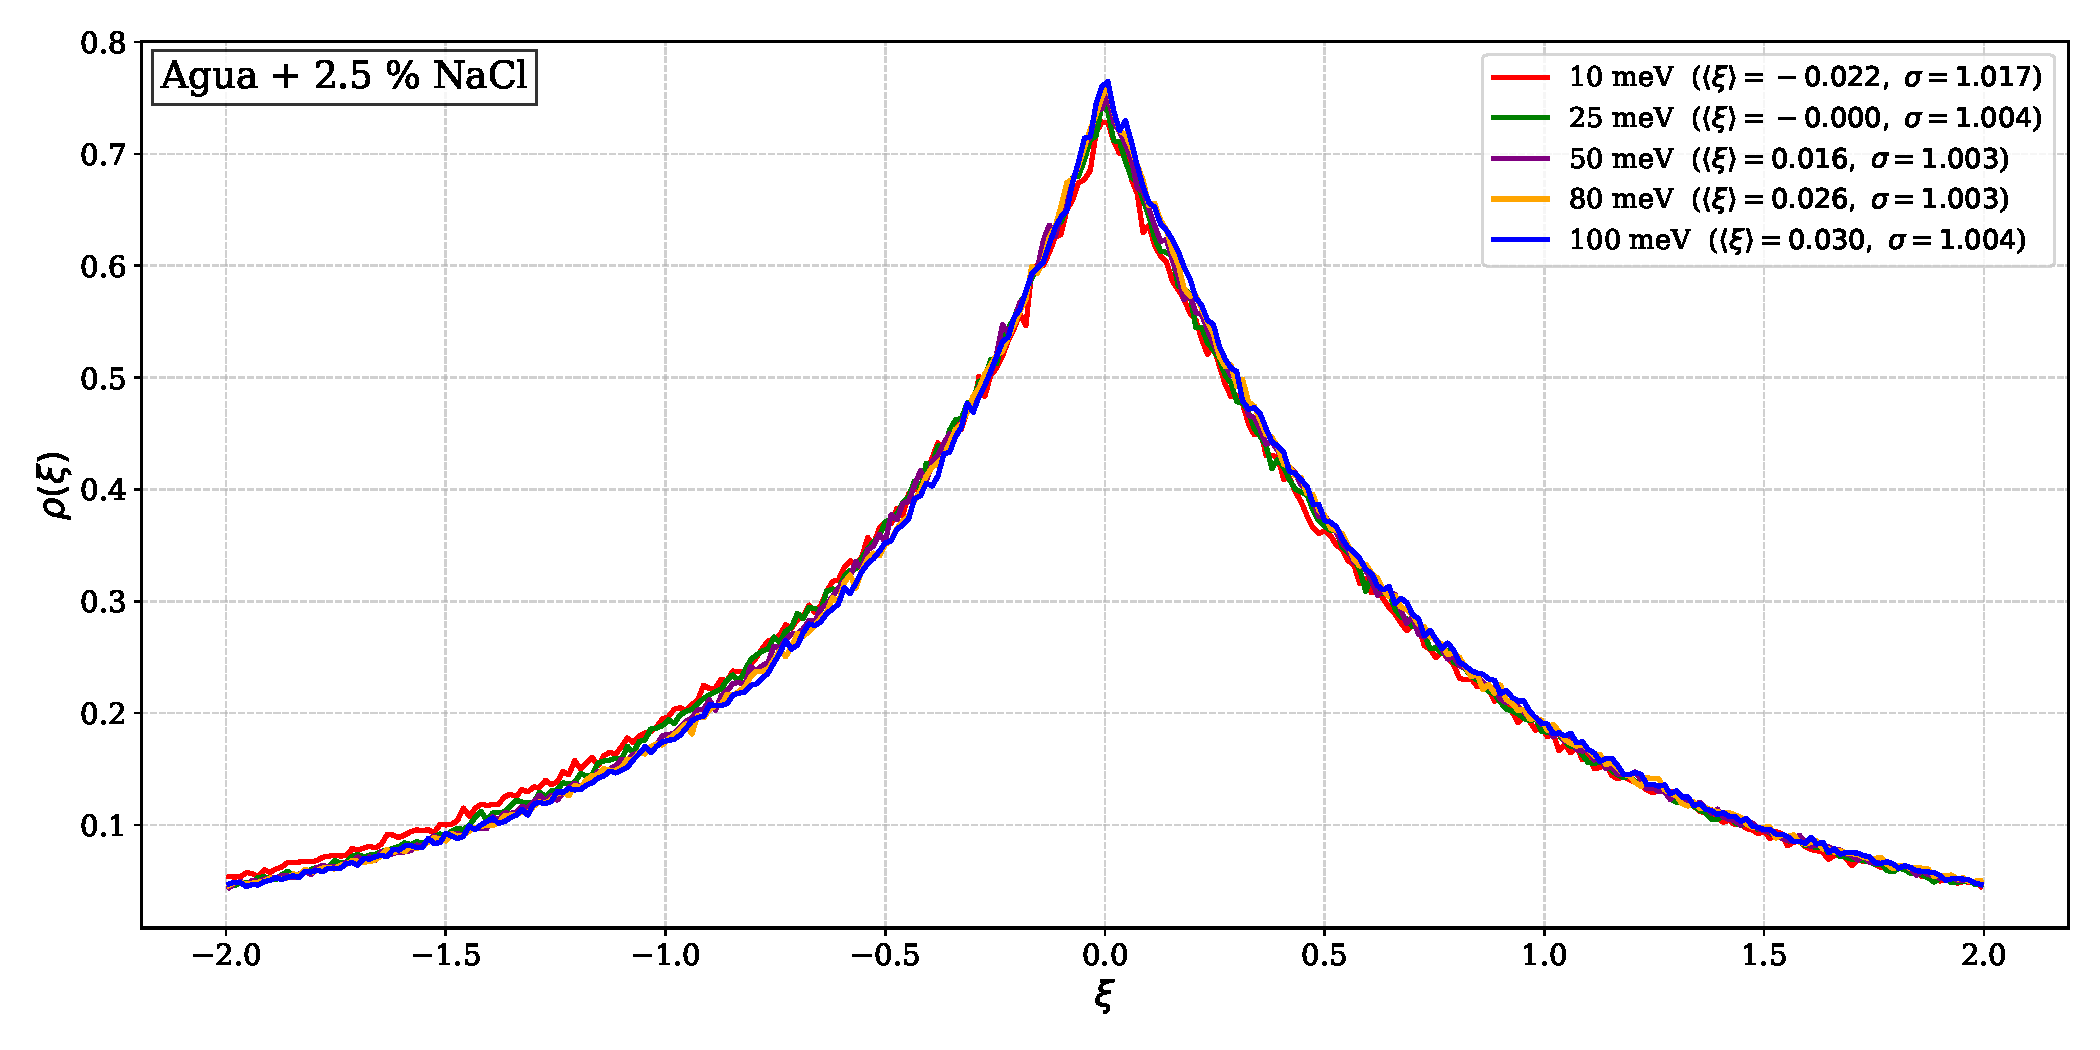
\includegraphics[width=0.72\linewidth]{fig_complementaria_xi_A25NaCl_termica.pdf}\\[0.2em]
  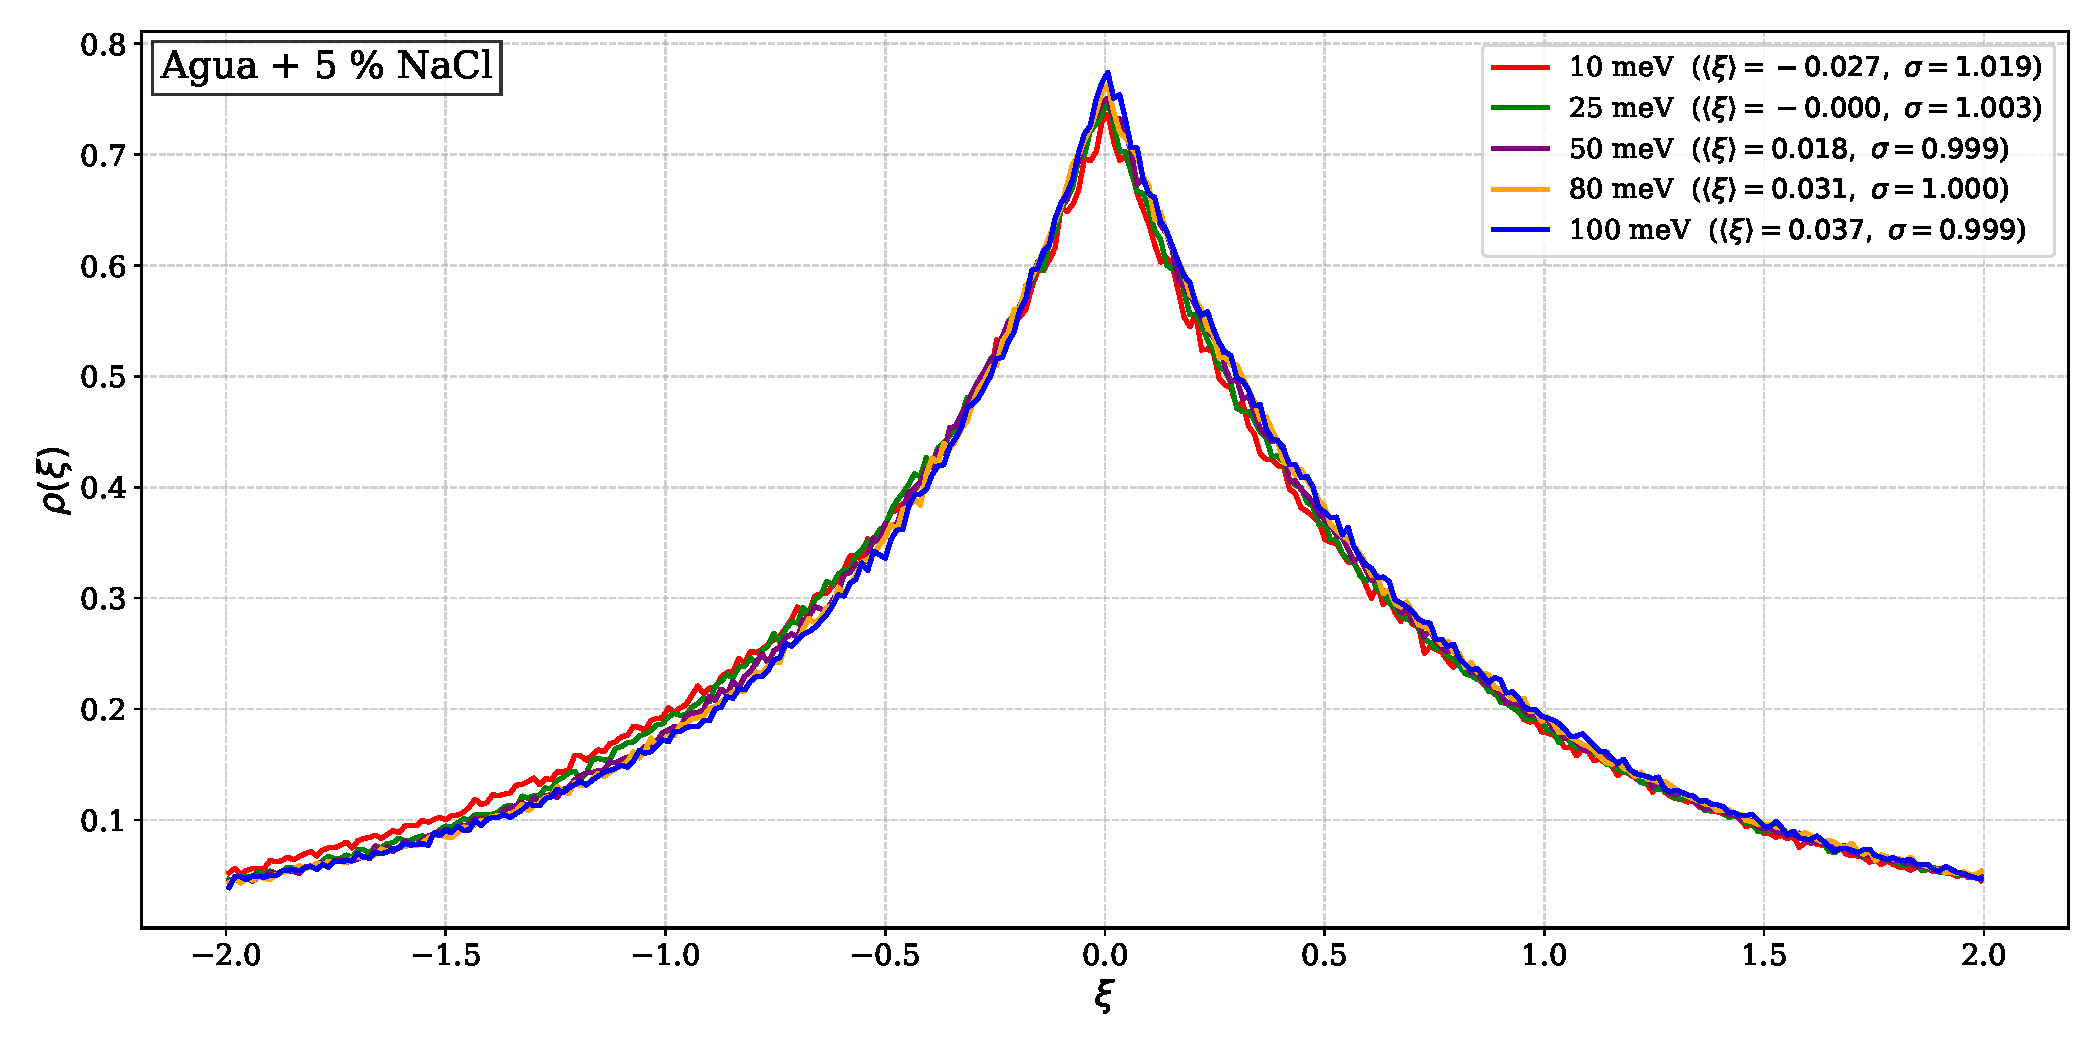
\includegraphics[width=0.72\linewidth]{fig_complementaria_xi_A5NaCl_termica.pdf}\\[0.2em]
  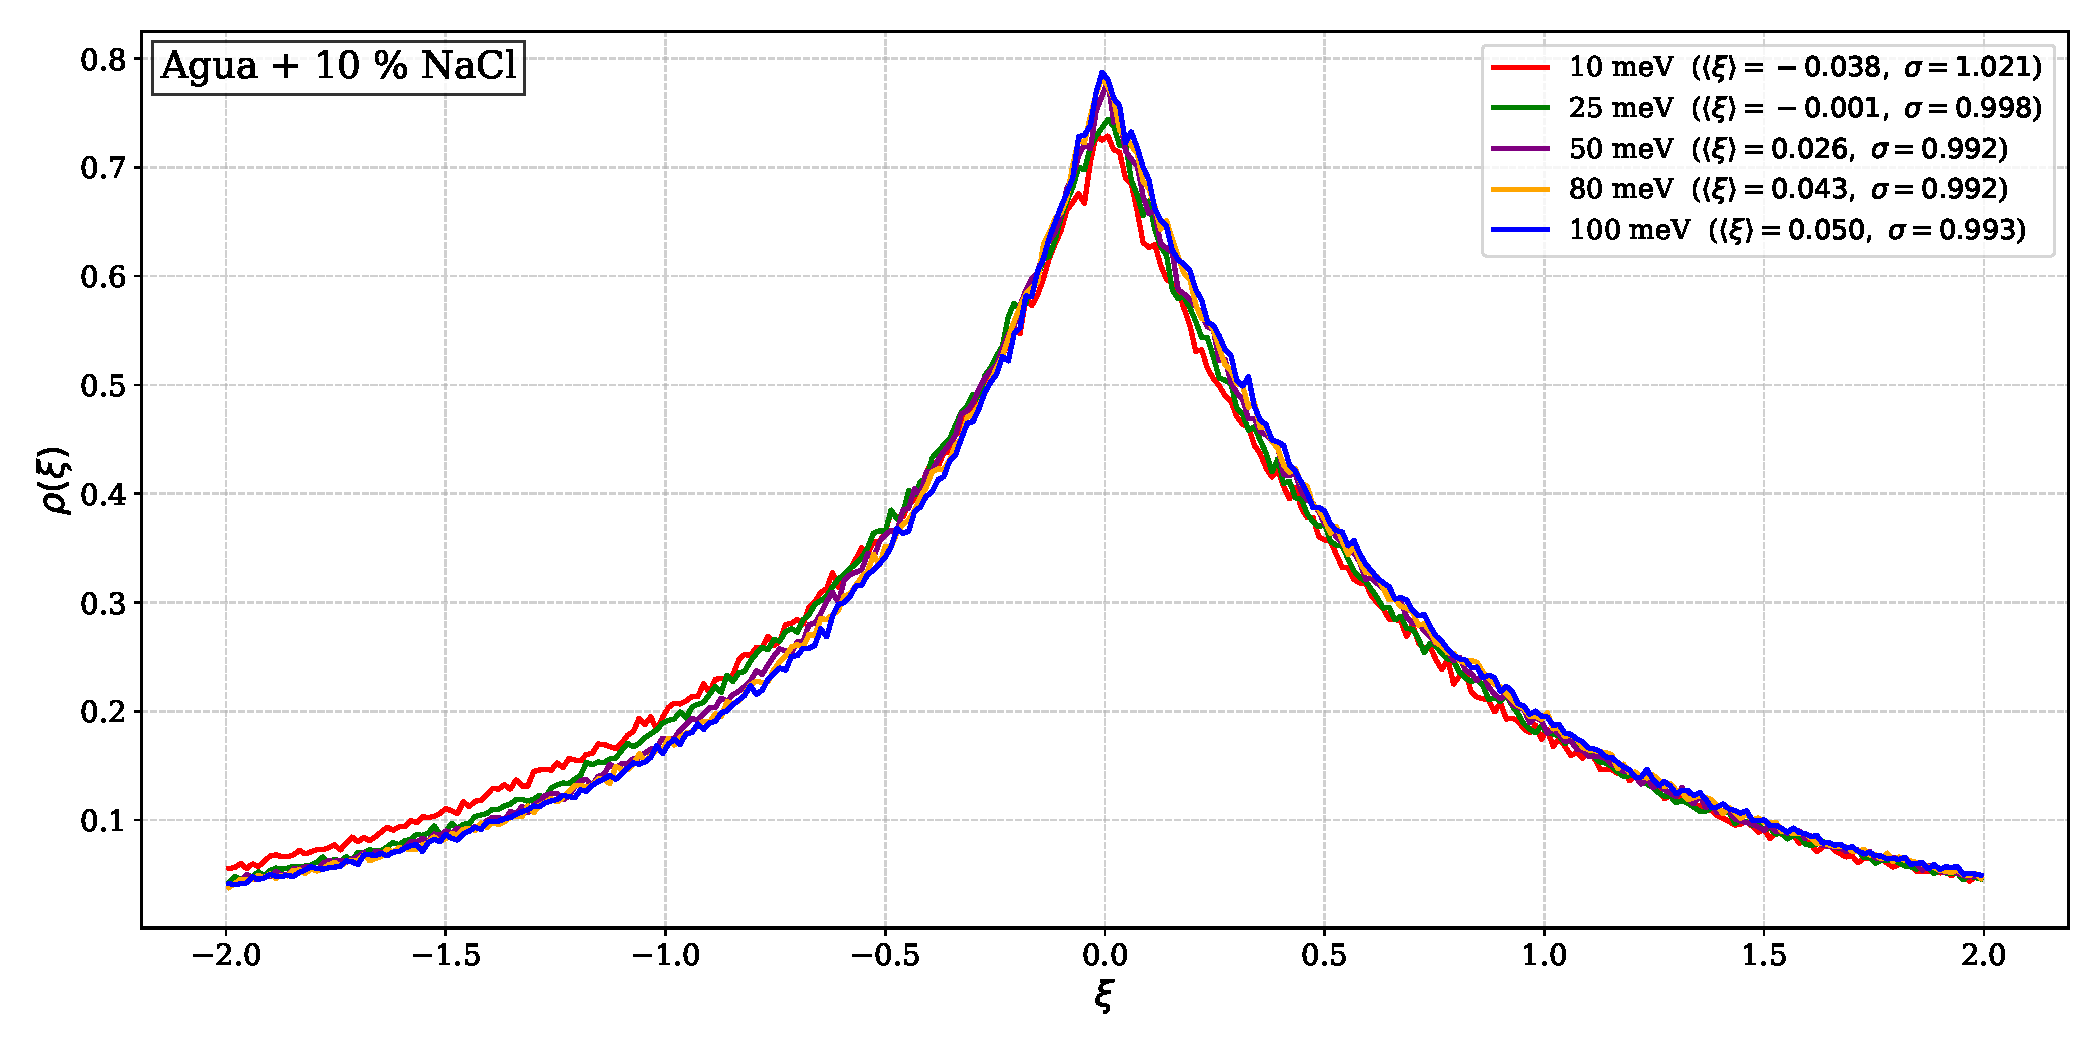
\includegraphics[width=0.72\linewidth]{fig_complementaria_xi_A10NaCl_termica.pdf}
  \caption{Distribución de $\xi$ en el régimen térmico para agua con 2.5, 5 y 10~\% de NaCl.}
\end{figure}

\begin{figure}[H]
  \centering
  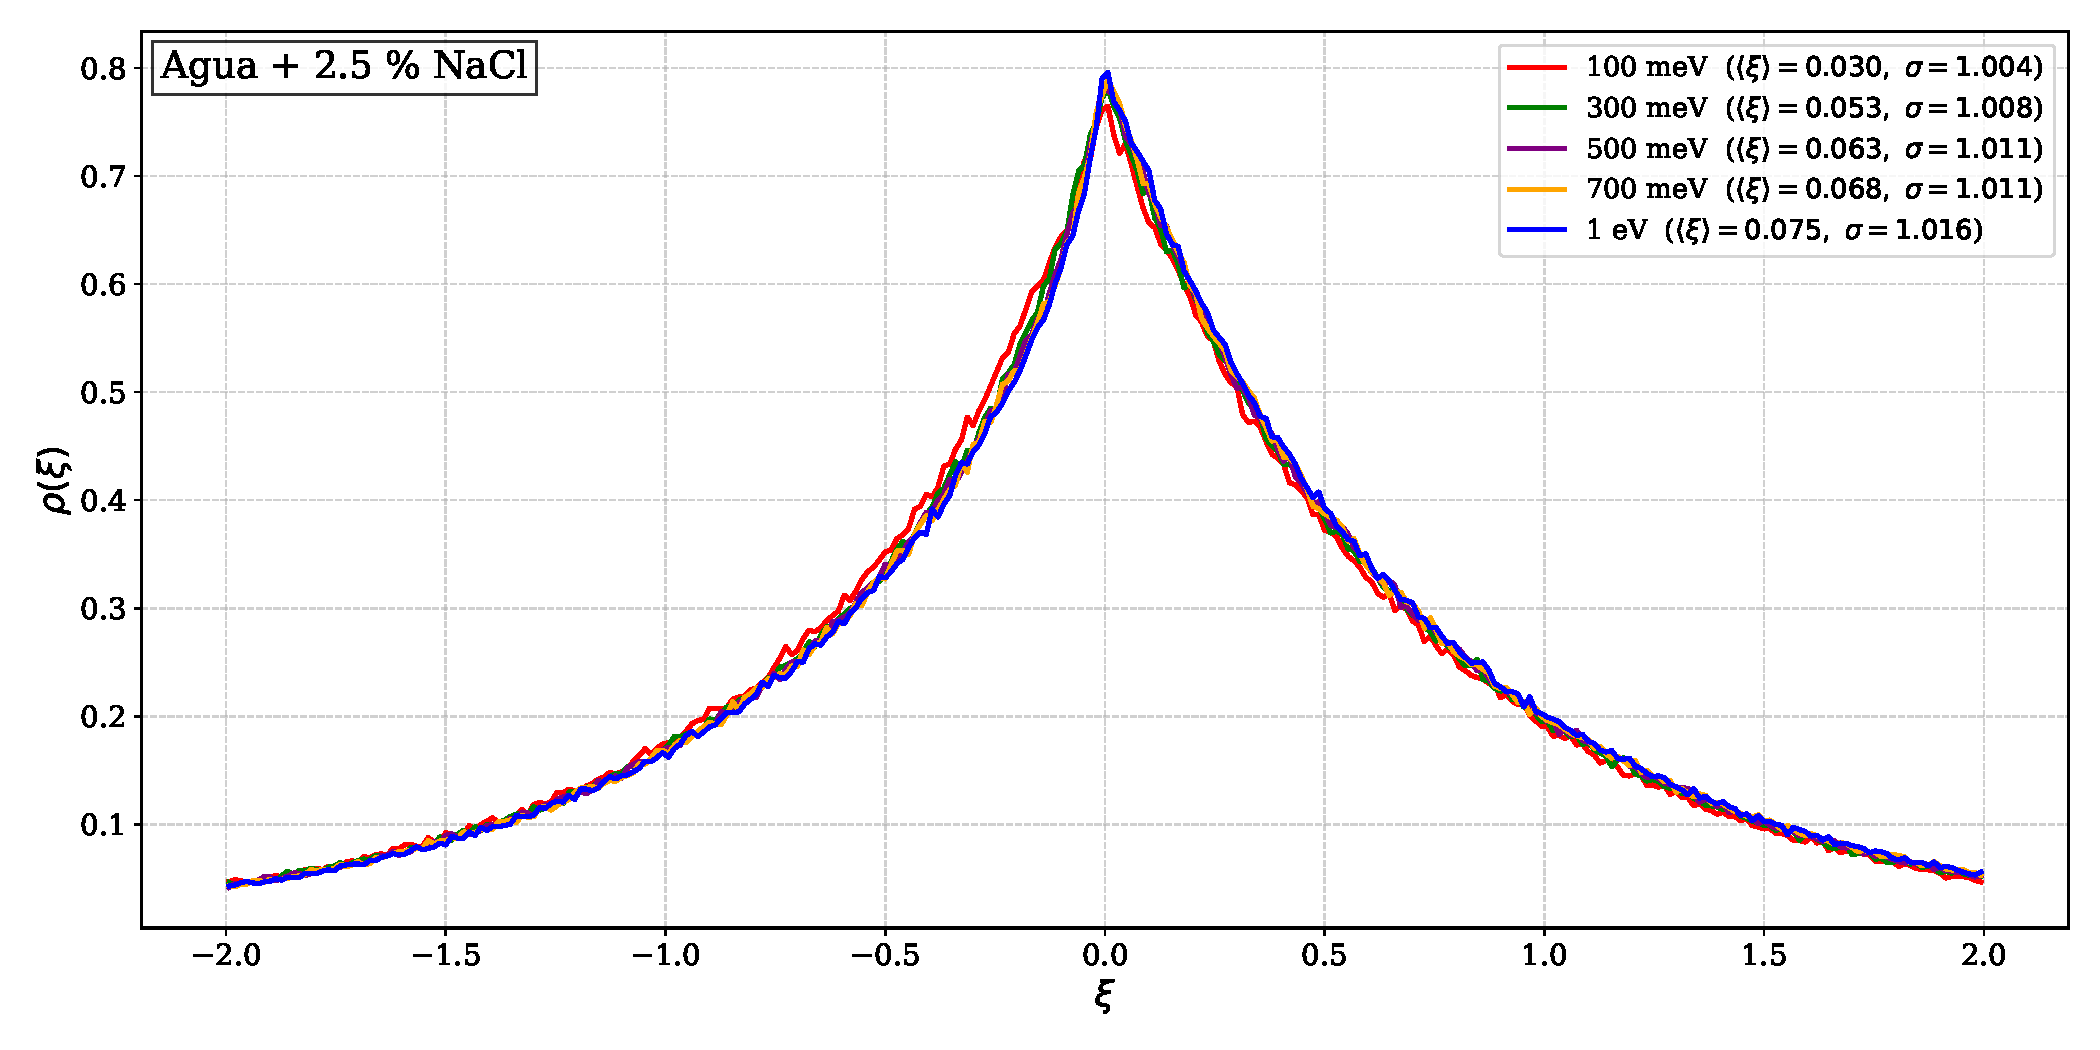
\includegraphics[width=0.72\linewidth]{fig_complementaria_xi_A25NaCl_epitermica.pdf}\\[0.2em]
  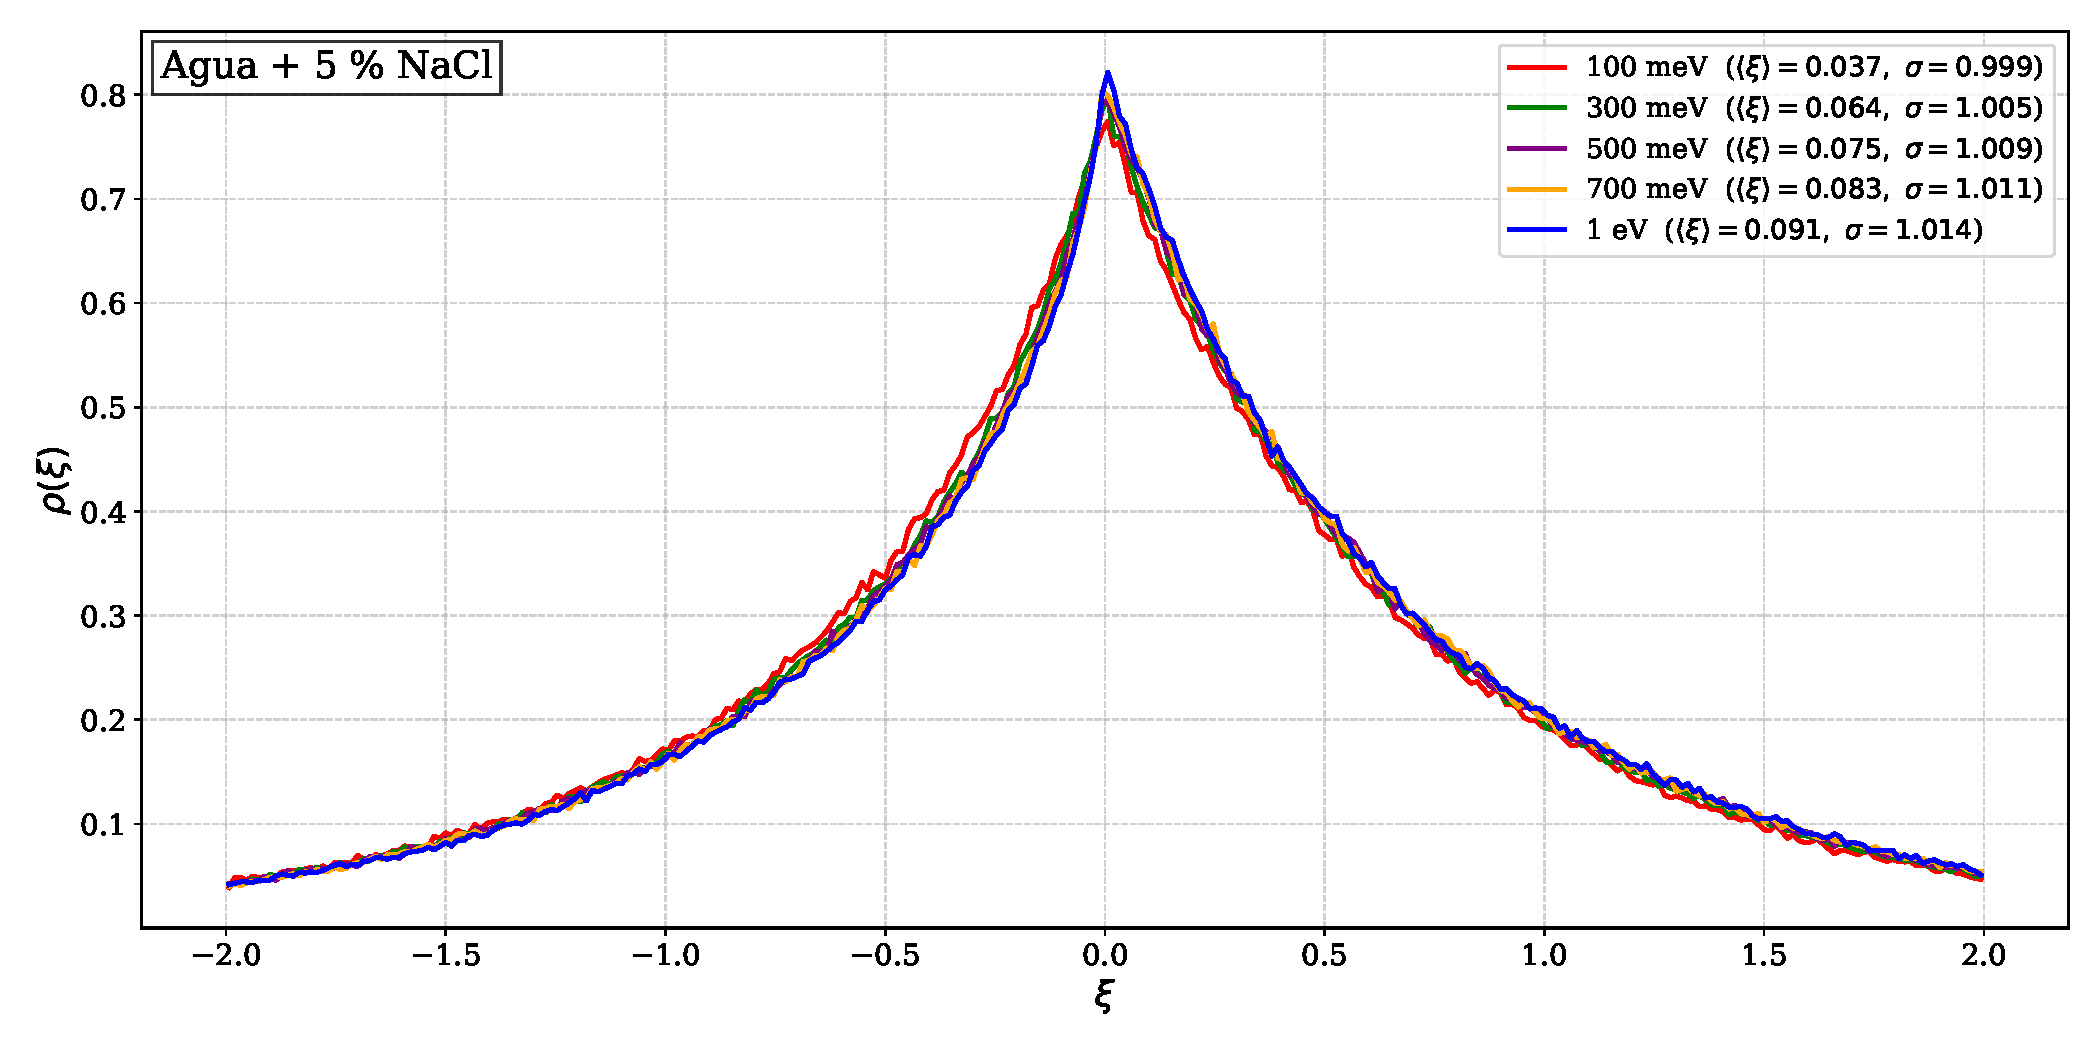
\includegraphics[width=0.72\linewidth]{fig_complementaria_xi_A5NaCl_epitermica.pdf}\\[0.2em]
  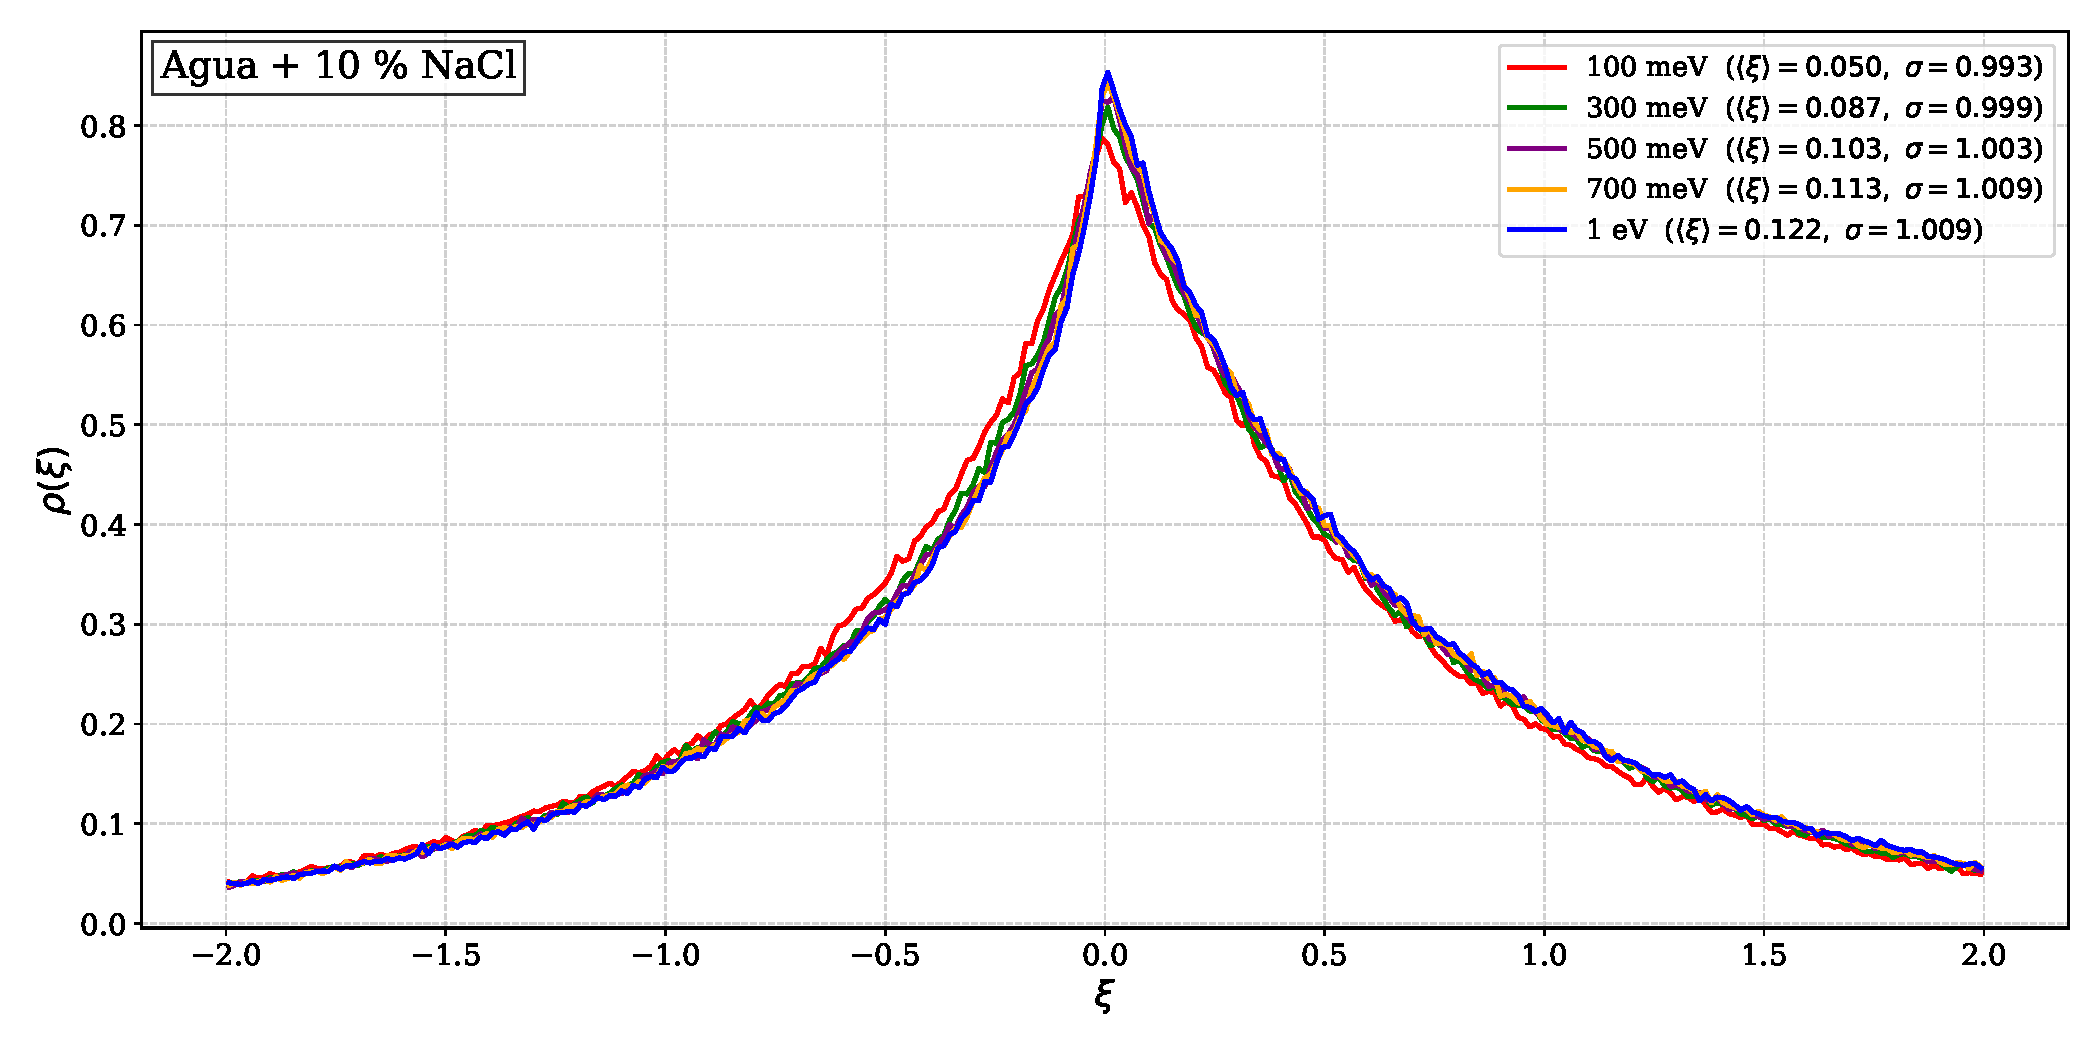
\includegraphics[width=0.72\linewidth]{fig_complementaria_xi_A10NaCl_epitermica.pdf}
  \caption{Distribución de $\xi$ en el régimen epitérmico para agua con 2.5, 5 y 10~\% de NaCl.}
\end{figure}

\begin{figure}[H]
  \centering
  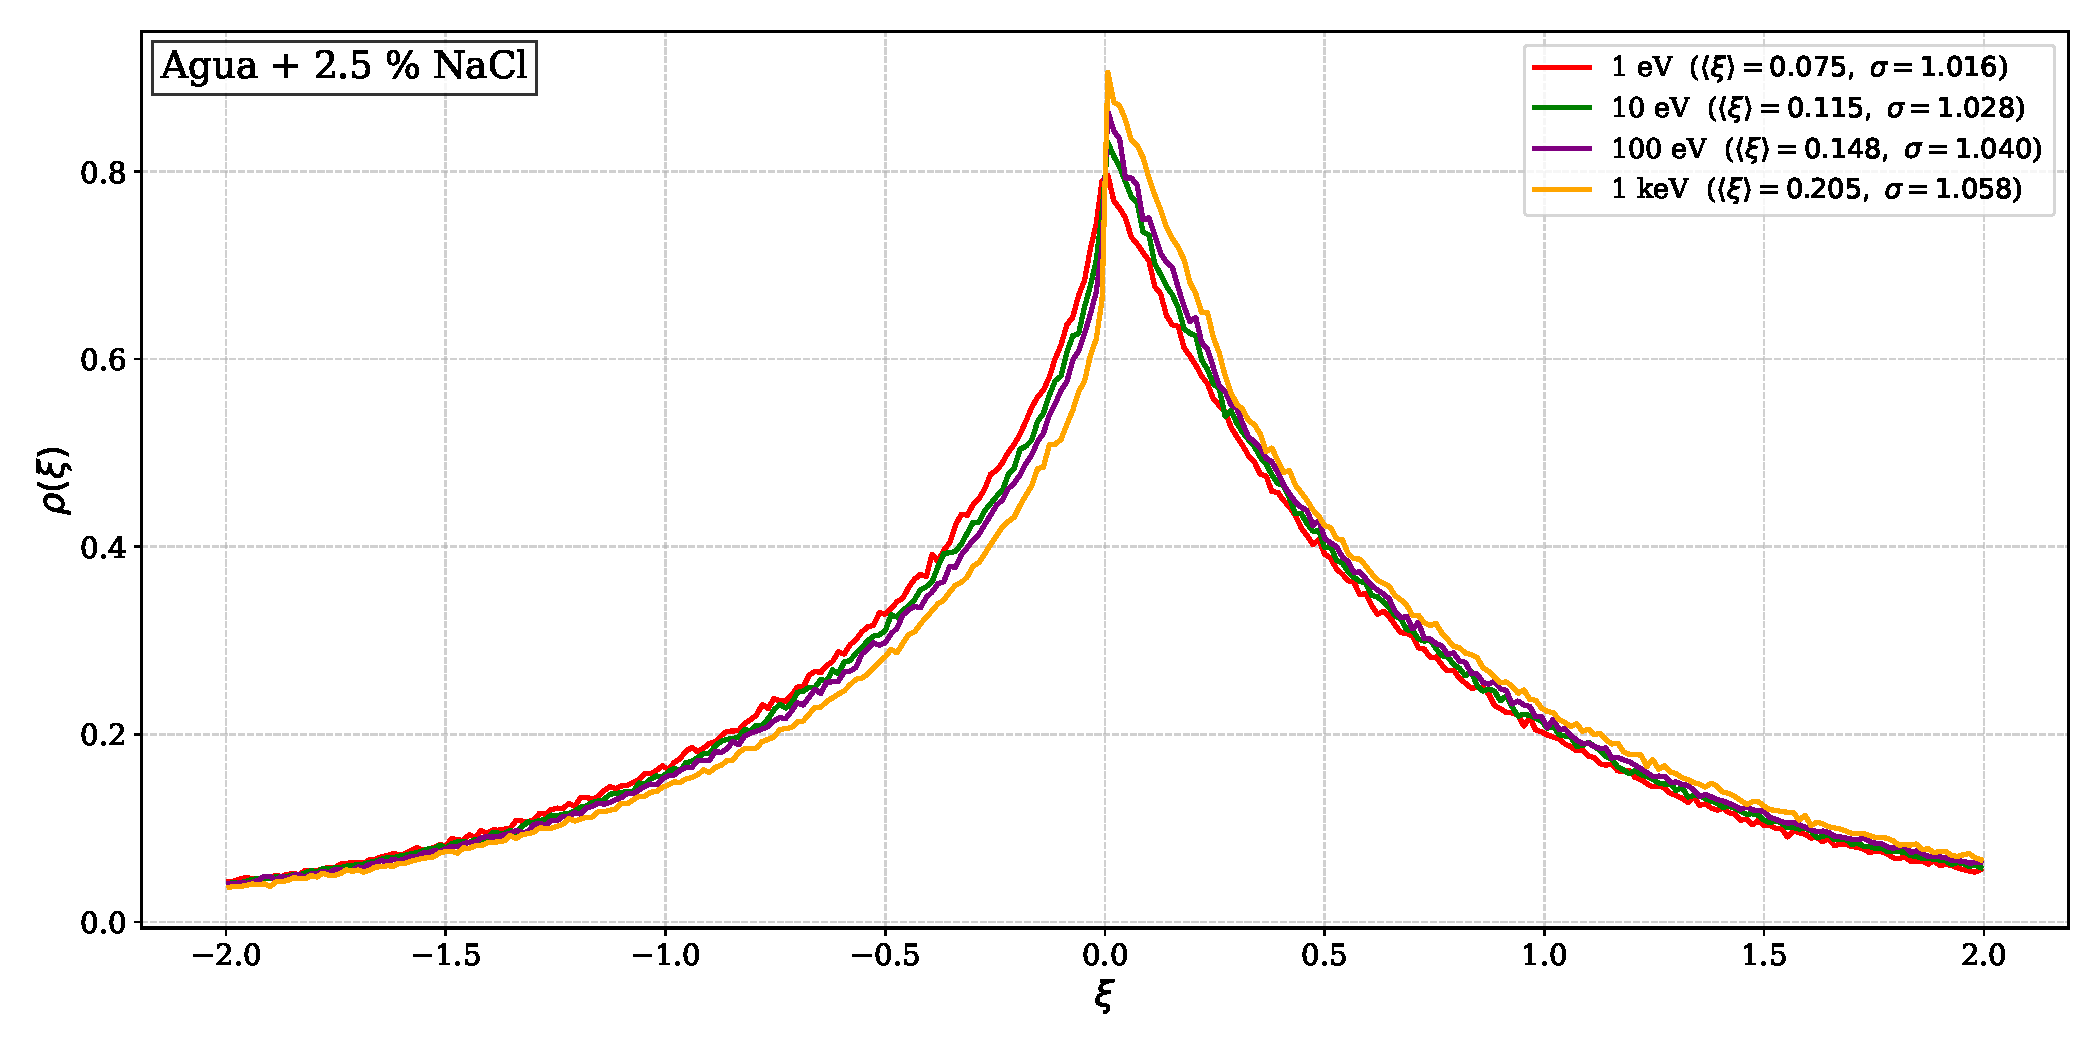
\includegraphics[width=0.72\linewidth]{fig_complementaria_xi_A25NaCl_intermedia.pdf}\\[0.2em]
  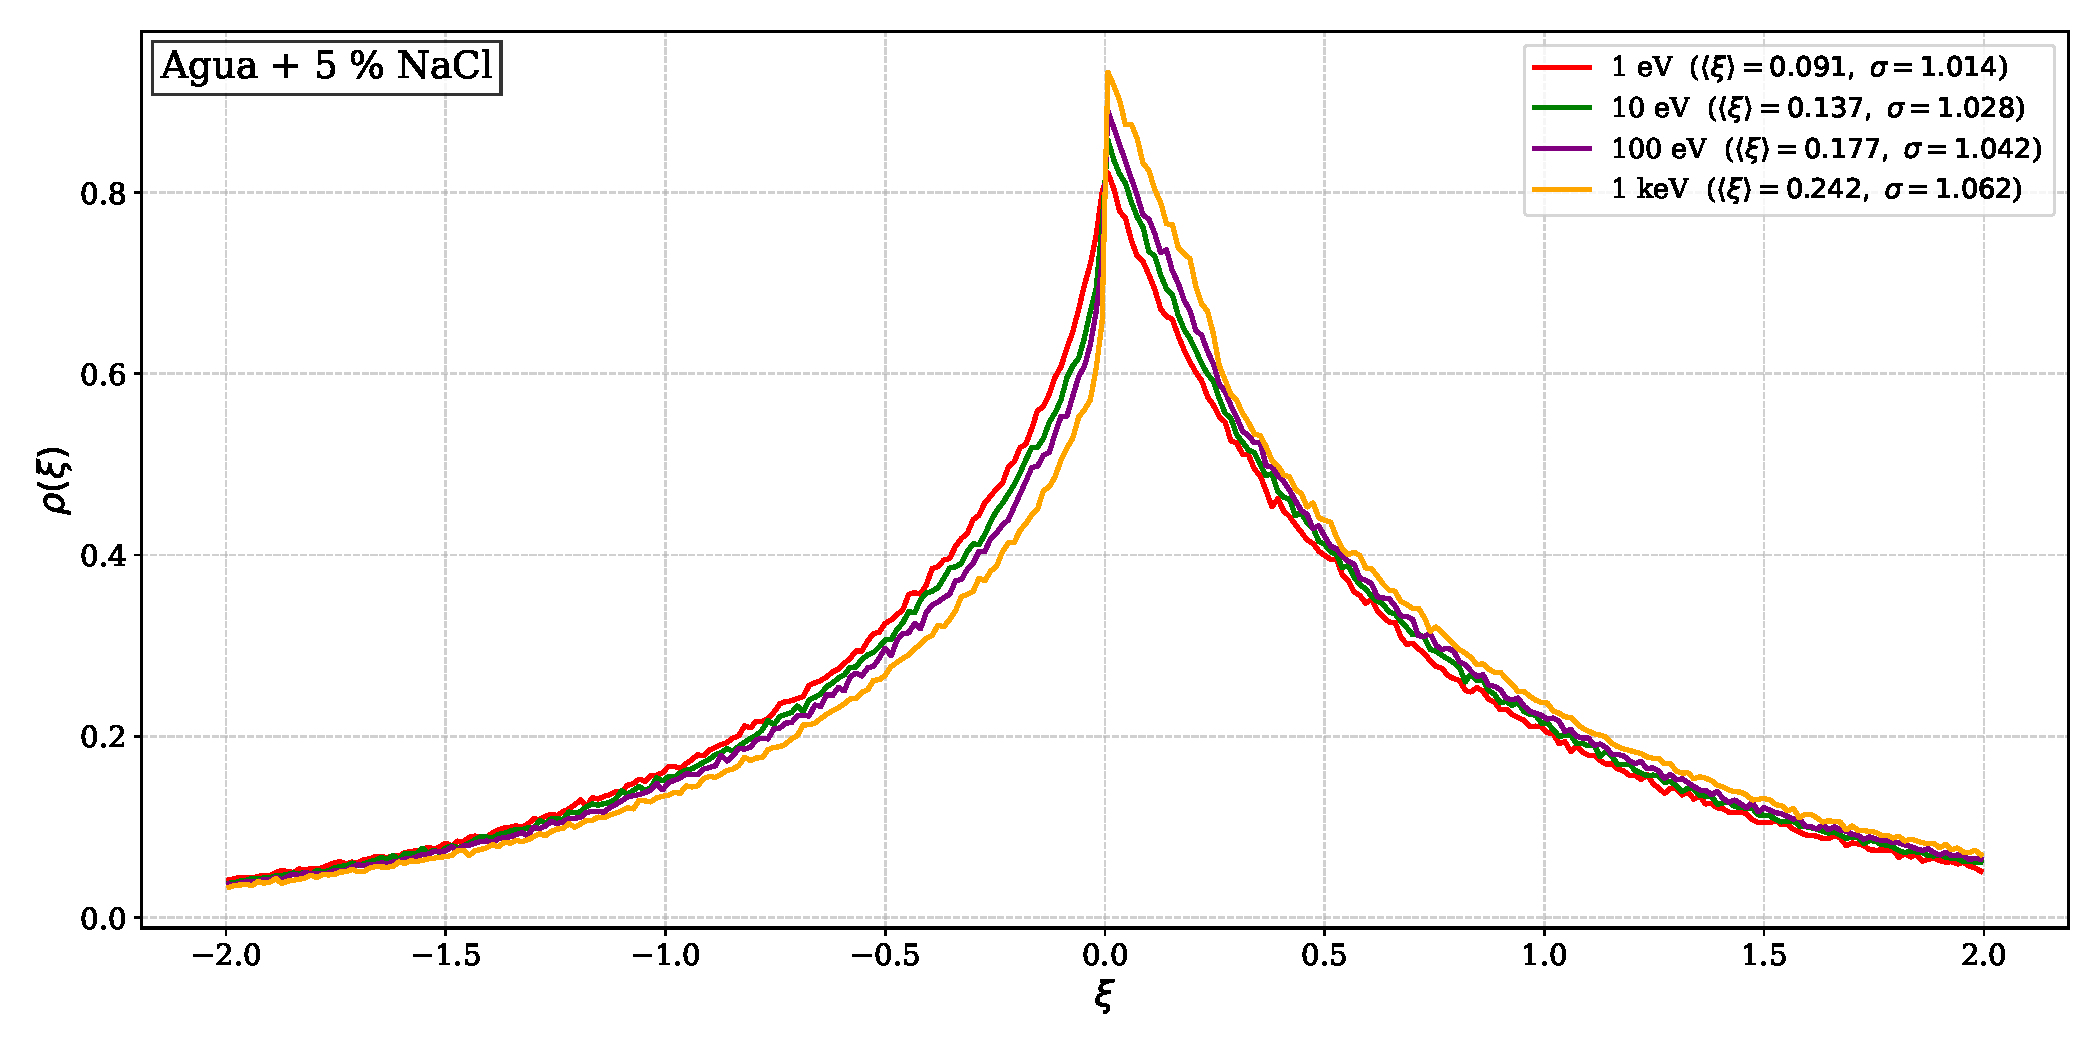
\includegraphics[width=0.72\linewidth]{fig_complementaria_xi_A5NaCl_intermedia.pdf}\\[0.2em]
  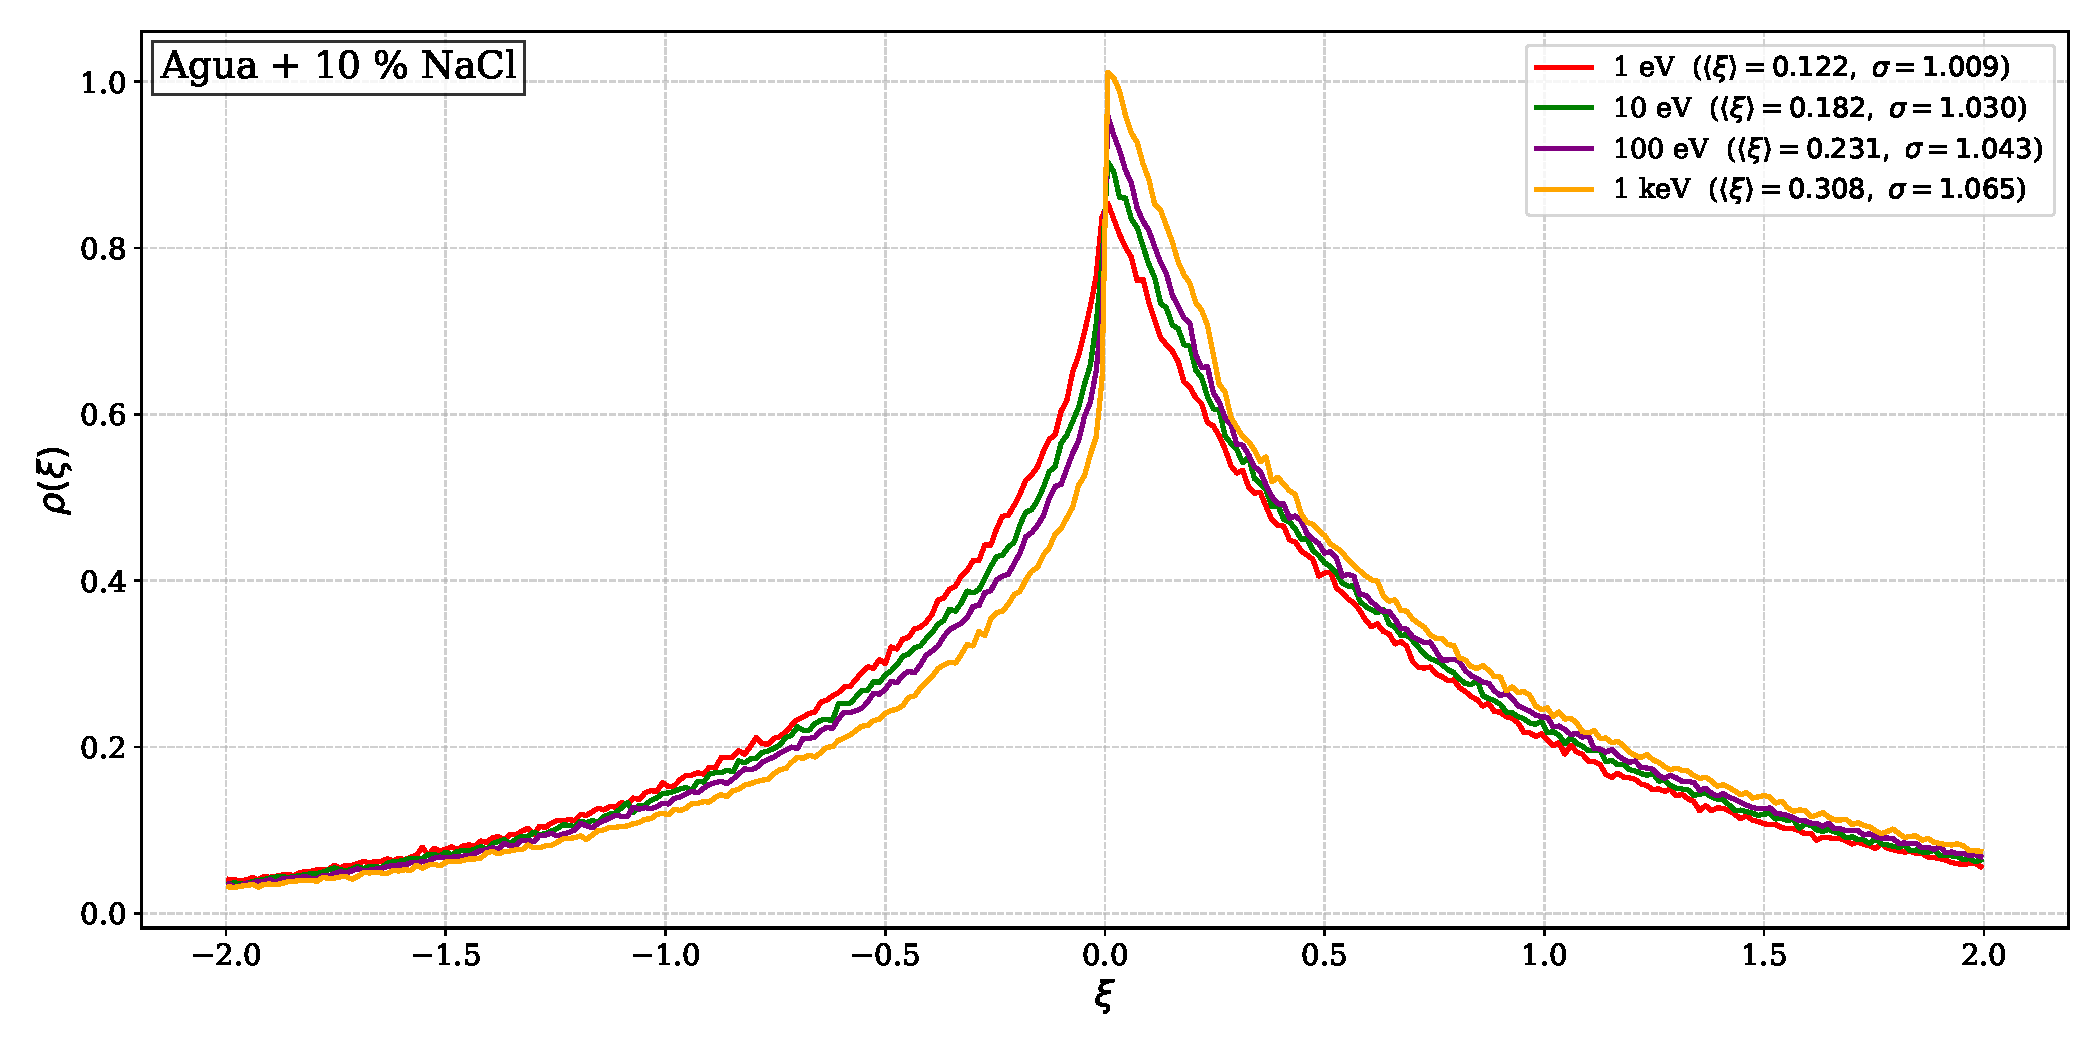
\includegraphics[width=0.72\linewidth]{fig_complementaria_xi_A10NaCl_intermedia.pdf}
  \caption{Distribución de $\xi$ en el régimen intermedio para agua con 2.5, 5 y 10~\% de NaCl.}
\end{figure}

% =====================================================================
\begin{thebibliography}{9}
\bibitem{Agostinelli2003} S.~Agostinelli \emph{et al.}, ``Geant4 --- a simulation toolkit'', \emph{Nucl.\ Instrum.\ Methods A} \textbf{506}, 250--303 (2003), doi:10.1016/S0168-9002(03)01368-8.
\bibitem{Allison2016} J.~Allison \emph{et al.}, ``Recent developments in Geant4'', \emph{Nucl.\ Instrum.\ Methods A} \textbf{835}, 186--225 (2016), doi:10.1016/j.nima.2016.06.125.
\bibitem{Kohli2015} M.~Köhli, M.~Schrön, M.~Zreda, U.~Schmidt, P.~Dietrich y S.~Zacharias, ``Footprint characteristics revised for field-scale soil moisture monitoring with cosmic-ray neutrons'', \emph{Water Resour.\ Res.} \textbf{51}, 5772--5790 (2015), doi:10.1002/2015WR017169.
\bibitem{Rogers1982} P.~S.~Z.~Rogers y K.~S.~Pitzer, ``Volumetric properties of aqueous sodium chloride solutions'', \emph{J.\ Phys.\ Chem.\ Ref.\ Data} \textbf{11}, 15--81 (1982), doi:10.1063/1.555660.
\bibitem{Tiesinga2021} E.~Tiesinga, P.~J.~Mohr, D.~B.~Newell y B.~N.~Taylor, ``CODATA recommended values of the fundamental physical constants: 2018'', \emph{Rev.\ Mod.\ Phys.} \textbf{93}, 025010 (2021), doi:10.1103/RevModPhys.93.025010.
\bibitem{Callen1985} H.~B.~Callen, \emph{Thermodynamics and an Introduction to Thermostatistics}, 2.\textsuperscript{a} ed., John Wiley \& Sons (1985).
\bibitem{Sidelnik2020} I.~Sidelnik \emph{et al.}, ``Simulation of 500 MeV neutrons by using NaCl doped water Cherenkov detector'', \emph{Adv.\ Space Res.} \textbf{65}, 2216--2222 (2020), doi:10.1016/j.asr.2020.02.024.
\bibitem{Knoll2010} G.~F.~Knoll, \emph{Radiation Detection and Measurement}, 4.\textsuperscript{a} ed., John Wiley \& Sons, Hoboken (2010).
\bibitem{Kohli2018} M.~Köhli, M.~Schrön y U.~Schmidt, ``Response functions for detectors in cosmic-ray neutron sensing'', \emph{Nucl.\ Instrum.\ Methods A} \textbf{902}, 184--189 (2018), doi:10.1016/j.nima.2018.06.052.
\end{thebibliography}

\end{document}
